 %Template by Nicolas RABREAU, Sarah PIERREL et Amélie AUDET,, modified by bibi

 
\documentclass[a4paper, 11pt, english]{report}
% -------------------------------------------------
% Language and Encoding
% -------------------------------------------------
\usepackage[utf8]{inputenc}       % UTF-8 encoding
\usepackage[T1]{fontenc}          % Font encoding
\usepackage[french]{babel}        % French language
	
% -------------------------------------------------
% Page Layout and Formatting
% -------------------------------------------------
\usepackage[left=2.5cm,right=2.5cm,top=3cm,bottom=3cm]{geometry}
\usepackage{fancyhdr}             % Header and footer customization
\pagestyle{fancy}
	%\renewcommand\headrulewidth{1pt}
\usepackage{parskip}              % Proper paragraph spacing
\setlength{\parindent}{20pt}
\setlength{\parskip}{15pt}
\usepackage{lastpage}             % Reference to the last page
\usepackage{titlesec}             % Section formatting
\usepackage{datetime}             % Date and time


% -------------------------------------------------
% Math Packages
% -------------------------------------------------
\usepackage{amsmath,amssymb,amsfonts} % Core math support
\usepackage{mathtools}                % Advanced math enhancements
\usepackage{icomma}                   % Comma spacing in math
\usepackage{esint}                    % Extended integral symbols
\usepackage[separate-uncertainty=true, per-mode=fraction]{siunitx} % SI units

% -------------------------------------------------
% Tables
% -------------------------------------------------
\usepackage{tabularx}           % Flexible tables
\usepackage{tabulary}           % Table width control
\usepackage{booktabs}           % Professional-quality tables
\usepackage{colortbl}           % Colored table rows
\newcommand{\myrowcolour}{\rowcolor[gray]{0.925}}
\usepackage{array, multirow}    % Advanced table formatting
\setlength\extrarowheight{2pt}
\usepackage{hhline}             % Horizontal lines
\usepackage{adjustbox}          % Content resizing

% -------------------------------------------------
% Graphics and Figures
% -------------------------------------------------
\usepackage{graphicx}           % Include images
\usepackage{caption}            % Caption customization
\usepackage{subfig}             % Subfigures
\usepackage{subcaption}         % Alternate subfigure support
\usepackage{wrapfig}            % Text wrapping around figures
\usepackage{tikz}               % Vector drawing
\usetikzlibrary{calc,arrows.meta}
\usetikzlibrary{decorations.pathmorphing} % pour zigzag
\usetikzlibrary{shapes.geometric} % formes

\usepackage{pgfgantt} % à ajouter dans le préambule si absent


\usepackage[RPvoltages]{circuitikz} % Circuit diagrams
\graphicspath{{Figures/},{equations/}} % Image search paths

% -------------------------------------------------
% Code Listings
% -------------------------------------------------
\usepackage{listings}           % Code listings
%\usepackage{minted}             % Syntax highlighting
\usepackage{xcolor}             % Custom colors
\definecolor{codegreen}{rgb}{0,0.6,0}
%\definecolor{codegray}{rgb}{0.5,0.5,0.5}
%\definecolor{codepurple}{rgb}{0.58,0,0.82}
%\definecolor{backcolour}{rgb}{0.95,0.95,0.92}

% -------------------------------------------------
% Bibliography and Glossary
% -------------------------------------------------
\usepackage[nonumberlist,acronym]{glossaries}

\makeglossaries
\bibliographystyle{plain}       % Numeric reference style

% -------------------------------------------------
% Hyperlinks
% -------------------------------------------------
\usepackage{hyperref}           % Hyperlinks
\usepackage{cleveref}
% -------------------------------------------------
% Miscellaneous
% -------------------------------------------------
\usepackage{enumitem}           % List customization
\usepackage{easylist}           % Simpler lists
\usepackage{textcomp}           % Extra text symbols
\usepackage{gensymb}            % Generic symbols
\usepackage{verbatim}           % Verbatim blocks
\usepackage{calligra}           % Calligraphy font
\usepackage{url}                % URL typesetting
\usepackage{placeins}           % Float placement control
\usepackage{comment}            % Comment out large blocks
\usepackage{float}

%\usepackage{textcomp}
% -------------------------------------------------
% Custom Commands
% -------------------------------------------------
\newcommand{\HRule}{\rule{\linewidth}{0.5mm}}
\NewDocumentCommand{\myrule}{O{1pt} O{2pt} O{black}}{%
  \par\nobreak
  \kern\the\prevdepth
  \kern#2
  {\color{#3}\hrule height #1 width\hsize}
  \kern#2
  \nointerlineskip
}

\newcommand{\red}{\textcolor{red}}
\newcommand{\blue}{\textcolor{blue}}
\newcommand{\ttt}{\texttt}
\newcommand{\itt}{\textit}
\newcommand{\ETT}{\textsc{embree2TRUST} }
\newcommand{\trust}{\textsc{TRUST} }
\newcommand{\pcr}{\textsc{pyMCRAD} }
\newcommand{\emb}{\textsc{INTEL EMBREE}\textsuperscript{\textcopyright}}
\newcommand{\mcrt}{Monte Carlo Ray Tracing }
\newcommand{\salome}{\textsc{SALOME} }
%%%%%%%%%%%%%%%%%%%%%%%%%%%
%after usepackage commands
%\bibliographystyle{ieeetr}

%%%%%%%%%%%%%%%%% TABLE OF CONTENTS %%%%%%%%%%%%%%%%%

\renewcommand{\listfigurename}{Table des figures} % Corrected label
\renewcommand{\contentsname}{Sommaire}


%%%%%%%%%%%%%%%%% HEADER / FOOTER CONFIGURATION %%%%%%%%%%%%%%%%%

\fancyhead[L]{\textbf{Rapport de stage}}
\fancyhead[C]{}
\fancyhead[R]{Antonin MONNERET}
\renewcommand\footrulewidth{1pt}
\fancyfoot[C]{\large Phelma - Septembre 2026}
\fancyfoot[R]{\textbf{ \thepage}}


\begin{document}
    % Title page
    
%%%%%%%%%%%%%%%%% TITLE PAGE %%%%%%%%%%%%%%%%%
\begin{titlepage}
    \centering
    %\vspace*{10cm}

    % Logos at the top
    \begin{minipage}{0.45\textwidth}
        \centering
        
\includegraphics[width=0.8\linewidth]{PICTURES/GINPPhelma.png} % First logo
    \end{minipage}%
    \hfill
    \begin{minipage}{0.45\textwidth}
        \centering
        
\includegraphics[width=0.6\linewidth]{PICTURES/CEA_logo_nouveau.png} % Second logo
    \end{minipage}

    \vspace{1.2cm}
    
    {\LARGE\bfseries Antonin MONNERET\par}
    %\vspace{0.1cm}
    {\large Génie Énergetique et Nucléaire: Stage de fin d'étude\par}
    %   \vspace{0.8cm}

    {\Large \textbf{Commisariat aux Énergies Atomiques et aux Énergies Nouvelles}\par
    \small CEA Paris-Saclay \\ DES/ISAS/DM2S/SGLS/LCAN \\ \par}
    \vspace{1.cm}

    { \Huge\bfseries Développement, vérification et étude \\d'un modèle de transfert radiatif en milieu transparent \\pour la plateforme \texttt{TRUST} \par}
    {\large du 30/03/26 au 21/08/26\par}
    
    % Optional image centered below the title
    % \includegraphics[width=0.4\textwidth]{illustration.png} % Uncomment if needed

    \vspace{0.2cm}
    \leftline{{\normalsize Sous la supervision de :\par}}
    \vspace{-0.2cm}
    {\footnotesize
    \begin{itemize}
        \item Maître de stage : Ansar Calloo, ansar.calloo@cea.fr
        \item Maître de stage : Romain Le Tellier, romain.letellier@cea.fr
        \item Maître de stage : Élie Saïkali, elie.saikali@cea.fr
    \end{itemize}
    \leftline{{\normalsize À destination de :\par}}
    \vspace{-0.2cm}
    \begin{itemize}
        \item Tuteur master : Merle Esla, merle@lpsc.in2p3.fr 
        \item Tuteur école : Giovanni Ghigliotti, ghigliotti@lpsc.in2p3.fr
    \end{itemize}
    }

    \vspace{0.5cm}
    \rightline{\large Confidentialité :   \LARGE\bfseries NON \par}
    \vfill

    \tiny{
    \leftline{\textcolor{gray}{\textbf{Ecole nationale supérieure de }}} 
    \leftline{\textcolor{gray}{\textbf{physique, électronique, matériaux}}}
    \vspace{0.2 cm}
    \leftline{\textcolor{red}{Phelma}}
    \leftline{Bât. Grenoble INP - Minatec}
    \vspace{0.2 cm}
    \leftline{3 Parvis Louis Néel - CS 50257}
    \leftline{38016 Grenoble Cedex 01}
    \vspace{0.2 cm}
    \leftline{Tél +33 (0)4 56 52 91 00}
    \leftline{Fax +33 (0)4 56 52 91 03}
    \vspace{0.2 cm}
    \leftline{\tiny {\textcolor{gray}{http://phelma.grenoble-inp.fr}}}}
    
\end{titlepage}

    \newpage 

    % Meditation time
    \rightline{\textit{\Large Spinoza Alain}}
\rightline{\textit{\Large others}}
\vspace{0.5 cm}

\rightline{Author}


\vfill
\leftline{\LARGE \bfseries Resume } 
\leftline{ A long time ago in a galaxy far, far away}

    % Sumario
    \newpage
    \tableofcontents

    %\addcontentsline{toc}{section}{Liste des acronymes}
    \printglossary[type=\acronymtype, title=Liste des acronymes]%, toctitle=Liste des acronymes]

    %\newpage
    \addcontentsline{toc}{section}{Liste des figures}
    \listoffigures

    %\newpage
    %\addcontentsline{toc}{section}{Liste des tableaux}
    \listoftables

    % End Sumario

    \newpage
    
    
    
    
%\newacronym{etr}{ETR}{Équation de Transfert Radiatif}
\section*{Glossaire}
\addcontentsline{toc}{chapter}{Glossaire}


\textbf{Bounding Volume Hierarchy (BVH)} — Structure de données hiérarchique utilisée par \textsc{Embree} pour accélérer la recherche d'intersections rayon-géométrie. Elle regroupe les éléments du maillage dans des boîtes englobantes imbriquées, permettant d'écarter rapidement de larges portions de la géométrie sans tester chaque triangle individuellement.

\textbf{Corium} — Mélange de matériaux fondus (combustible, gaines, structures) formé lors de la fusion du cœur d'un réacteur en situation accidentelle grave, notamment lors d'un accident de perte de réfrigérant primaire.

\textbf{\emb} — Bibliothèque logicielle développée pour l'accélération des calculs d'intersection rayon-géométrie sur architecture CPU, utilisée dans ce rapport pour le traitement géométrique des trajectoires de rayons du module Monte Carlo.

\textbf{\ETT} — Nom du module de calcul radiatif par lancer de rayons Monte Carlo développé au cours de ce stage, couplé à la plateforme \trust.

\textbf{Facteur de vue} — Grandeur géométrique sans dimension représentant la fraction du rayonnement quittant une surface qui est interceptée par une autre surface. Noté $F_{ij}$, il dépend uniquement de la géométrie relative des deux surfaces considérées.

\textbf{Facteurs de Gebhart} — Modèle de calcul à zones prenant en compte les réflexions multiples entre surfaces, mentionné dans le cadre des travaux antérieurs sur le couplage conduction-rayonnement.

\textbf{Hypersensibilité (problème hyper-sensible)} — Caractéristique de certains problèmes radiatifs pour lesquels une faible erreur sur les facteurs de vue engendre une erreur bien plus importante sur le flux radiatif après propagation, nécessitant une précision très fine des facteurs de vue (par exemple $10^{-4}$ pour obtenir $5\,\%$ de précision sur le flux dans certains cas).

\textbf{HTGR / VHTR} — \textit{High Temperature Gas-cooled Reactor} / \textit{Very High Temperature Reactor} : filières de réacteurs nucléaires utilisant l'hélium comme caloporteur et le graphite comme modérateur, fonctionnant à des températures de sortie comprises entre $750\,^\circ$C et $950\,^\circ$C.

\textbf{Hypothèse de Boussinesq} — Approximation couramment utilisée en mécanique des fluides, consistant à négliger les variations de masse volumique du fluide sauf dans le terme de flottabilité (gravité), simplifiant ainsi la résolution des écoulements à convection naturelle.

\textbf{MG-CADSurf / MG-Tetra} — Algorithmes de maillage de la plateforme \salome, utilisés respectivement pour générer le maillage surfacique (triangulaire) et le maillage volumique (tétraédrique) des géométries étudiées.

\textbf{Monte Carlo Ray Tracing (MCRT)} — Méthode numérique de calcul des facteurs de vue et des échanges radiatifs par lancer aléatoire d'un grand nombre de rayons, particulièrement adaptée aux géométries tridimensionnelles complexes.

\textbf{PyMCRad} — Code de référence utilisé pour la vérification par comparaison des résultats du module développé au cours de ce stage.

\textbf{Radiosité} — Grandeur ($J$, en W/m²) représentant l'ensemble de l'énergie rayonnée quittant une surface, somme de sa puissance émissive propre et de la fraction réfléchie du rayonnement incident (irradiance).

\textbf{Radiosité uniforme (hypothèse, modèle d'ordre 1)} — Hypothèse selon laquelle la radiosité est supposée constante sur l'ensemble d'une surface donnée, ce qui permet d'introduire les facteurs de vue mais introduit un biais d'autant plus important que la surface présente de forts gradients de température.

\textbf{RRMSE (\textit{Relative Root Mean Square Error})} — Métrique d'erreur quadratique moyenne relative, utilisée dans ce rapport pour quantifier globalement l'écart entre une matrice de facteurs de vue calculée et une matrice de référence.

\textbf{\salome} — Plateforme logicielle du CEA utilisée pour la génération de maillages (surfaciques et volumiques) et le prétraitement géométrique des cas de simulation, notamment via le format de fichier \texttt{.med}.

\textbf{Star-Engine} — Moteur de lancer de rayons développé par la société Meso-Star, s'appuyant sur \textsc{Embree}, dont l'observation a motivé le choix de cette bibliothèque pour le développement du module \ETT.

\textbf{\trust} — Plateforme multiphysique de calcul scientifique développée au CEA, utilisée pour la résolution des problèmes thermohydrauliques couplés à la simulation radiative dans ce rapport.

\textbf{TRISO} — Type de particule combustible enrobée (\textit{TRi-structural ISOtropic}) utilisée dans les réacteurs HTGR, offrant une bonne stabilité thermique et mécanique.
    \subsection*{Contexte technologique}

Les transferts radiatifs présentent une forte dépendance à la température. La loi de Stefan-Boltzmann montre que la puissance surfacique émise par un corps noir est proportionnelle à la quatrième puissance de sa température absolue. À titre d'exemple, cette puissance passe d'environ 420~W\,m$^{-2}$ à température ambiante à près de 75~kW\,m$^{-2}$ pour une température de 800~°C. Le rayonnement thermique constitue ainsi un mode de transfert de chaleur prépondérant dès lors que les températures deviennent élevées.

Ces phénomènes interviennent dans de nombreuses technologies nucléaires. Les réacteurs à très haute température (VHTR) et les réacteurs refroidis au gaz en sont des exemples emblématiques, le rayonnement participant de manière significative aux échanges thermiques au sein du cœur. Cette problématique est au cœur de plusieurs développements récents, depuis la mise en service de la centrale \textit{Shidao Bay} en Chine jusqu'au développement du concept de micro-réacteur calogène \textit{Jimmy}. 
Le rayonnement thermique joue également un rôle essentiel dans l'analyse des situations accidentelles des réacteurs à eau sous pression (REP) et des réacteurs à eau bouillante (REB). Lors d'un accident de perte de réfrigérant primaire, la température du cœur peut atteindre plusieurs milliers de kelvins. De telles conditions conduisent à une dégradation progressive des matériaux, depuis l'oxydation des gaines jusqu'à la fusion du combustible et à la formation de corium.

L'étude de ces phénomènes repose sur une complémentarité entre les approches expérimentales et la simulation numérique. Cette dernière mobilise des modèles physiques adaptés à la diversité des milieux rencontrés, qu'il s'agisse de milieux transparents, semi-transparents ou participants.

\subsection*{Enjeu du stage}

Le présent stage s'inscrit dans le cadre du transfert radiatif entre surfaces opaques séparées par un milieu transparent. Cette configuration constitue une hypothèse classique dans de nombreux modèles de milieux poreux, notamment ceux proposés dans \cite{Romain25} et \cite{chahlafi}. Les travaux réalisés reposent sur un code de Monte Carlo par lancer de rayons (\textit{Monte Carlo Ray Tracing}, MCRT). Ils ont consisté à reprendre une première maquette développée lors d'un précédent stage, à en consolider les fondements numériques et logiciels, puis à utiliser un module permettant son couplage avec les autres modes de transfert de chaleur au sein de la plateforme TRUST \cite{saikali2025trust}.

Ce rapport est organisé de la manière suivante. Le premier chapitre présente les fondements physiques du transfert radiatif dans les hypothèses retenues (Section~\ref{part:c1}). Le deuxième chapitre décrit le développement du code de calcul ainsi que les méthodes numériques mises en œuvre (Section~\ref{part:c2}). Le troisième chapitre est consacré à la vérification du module développé au moyen de solutions analytiques (Section~\ref{part:q}) et de comparaisons avec le code de référence PyMCRad (Section~\ref{part:pymcrad}). Enfin, le dernier chapitre étudie l'influence de la discrétisation géométrique sur la précision des flux themiques (Section~\ref{part:c4}).


	
	\chapter{Approche théorique}
\section{Bilan radiatif en milieu transparent entre surfaces opaques}

\newpage
\section{Bilan radiatif en milieu transparent entre surfaces opaques}
L'objectif de cette partie est d'exprimer le flux radiatif $q$~[W/m²] sortant de chaque face solide, afin de prendre en compte le rayonnement dans les transferts thermiques. Plusieurs phénomènes sont à prendre en compte simultanément dans un problème radiatif: l'émission du système (qui suit la loi de Stefan Boltzmann) ainsi que la transmission, l'absorption et la réflexion de l'énergie irradiée. Plusieurs hypothèses courantes permettent de simplifier la définition des domaines physiques. La remise en cause de ces hypothèses ne rentre pas dans le cadre de ce travail, mais pourra nourrir la discussion d'un projet futur.


\subsection{Formulation du problème}
On considère ici que le rayonnement se fait entre des surfaces solides opaques au travers d'un milieu transparent. La première hypothèse est la transparence du fluide, i.e. il n'absorbe, n'émet ni réfléchi de rayonnement.


L'hypothèse d'opacité des surfaces permet de négliger la transmission dans ces milieux. Le rayonnement incident, aussi appelé l'irradiance ($G$~[W/m²]) est donc réfléchi ou absorbé. On obtient alors la complémentarité des coefficients de réflexion et d'absorption : $\forall \lambda, \, \rho_{\lambda} + \alpha_{\lambda} = 1$. On suppose ensuite que les surfaces sont grises: les coefficients $\alpha$ et $\epsilon$ sont indépendants de la longueur d'onde $\lambda$. La radiosité $J$~[W/m²] s'écrit alors comme la somme de la puissance émissive $E$~[W/m²] et de la réflexion de l'irradiance $\rho G$ : 
\begin{equation}
    \forall \vec{r}_i \in \text{Surface}_i, \quad J_i(\vec{r_i}) = \epsilon_i \sigma \big(T(\vec{r}_i)\big)^4 + \rho_i G_i(\vec{r_i})
\label{def:radiosite}
\end{equation} 

Avec $\epsilon_i$ (resp. $\rho_i$) l’émissivité (resp. la réflectivité) de la surface $i$, $\sigma$ désigne la constante de Stefan-Boltzmann et $T_i(\vec{r}_i$ la température de la surface $i$ à la position $\vec{r}_i$. La radiosité correspond à l'ensemble de l'énergie radiée qui quitte une surface. Le flux radiatif en surface peut ainsi s'écrire grâce à un  bilan comme représenté sur la Figure \ref{fig:radio}:
\begin{equation}
    \forall \vec{r}_i \in \text{Surface}_i,\quad q_i(\vec{r}_i) =  J(\vec{r}_i)  - G(\vec{r}_i) 
    \label{eq:qr}
\end{equation}

 Enfin, on suppose que l'irradiation et les surfaces sont diffuses. On a alors $G_{\lambda, i} (\lambda, \theta, \varphi)$ est indépendant de $\lambda$, $\theta$ et $\varphi$ et comme le montre la Figure \ref{fig:diffus}.

%\textit{Loi de Kirchhoff : alpha = espilon si isoT+ petit corps dans une cavité, eq thermique}

\begin{minipage}{0.45\textwidth}
    \centering
    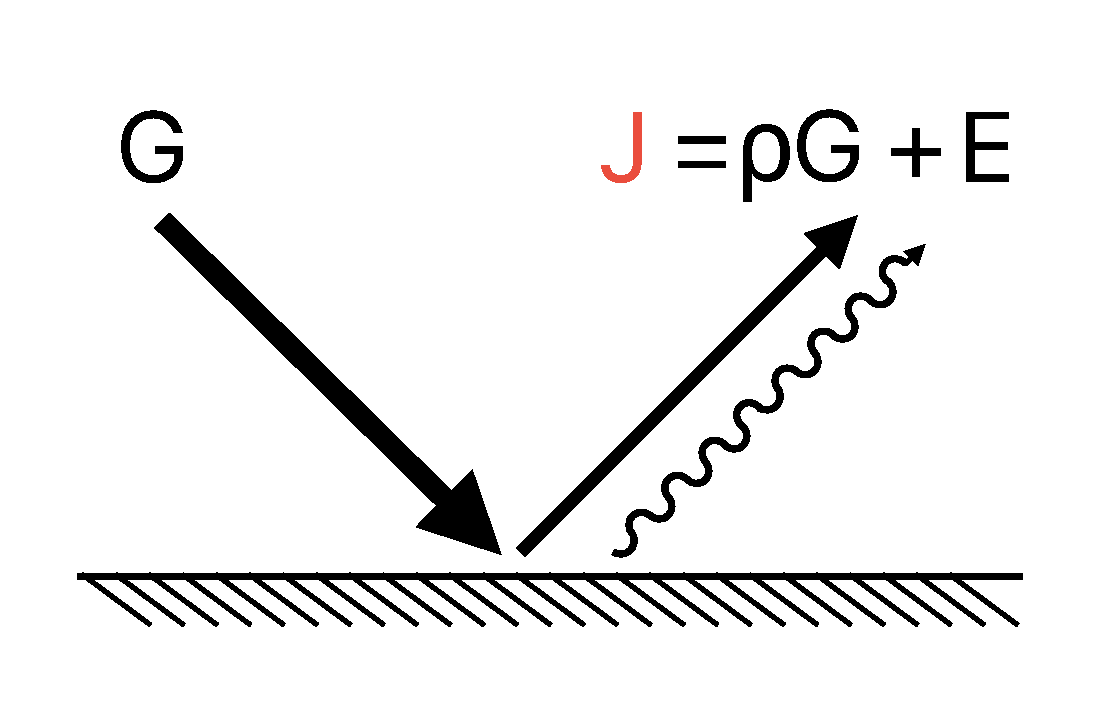
\includegraphics[width=0.9\linewidth]{PICTURES/radiosite.pdf}
    \captionof{figure}{Échanges radiatifs considérés dans le problème}
    \label{fig:radio}
\end{minipage}
\hfill
\begin{minipage}{0.45\textwidth}
    \centering
    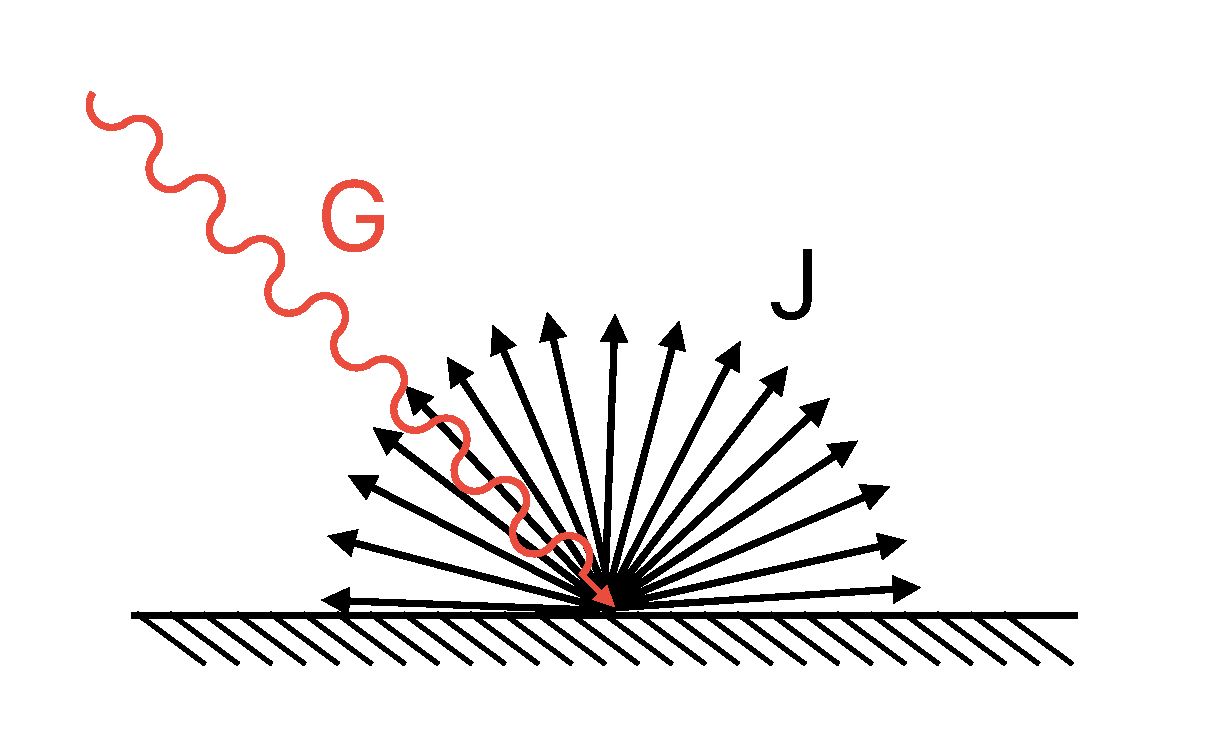
\includegraphics[width=0.9\linewidth]{PICTURES/diffus.pdf}
    \captionof{figure}{Illustration de l'hypothèse de réflexion et émission diffuse}
    \label{fig:diffus}
\end{minipage}





Pour finir, l’irradiance est exprimée conformément à la Figure \ref{fig:fij_schema} en fonction des radiosités sous la forme : 
\begin{equation}
    \forall i \in [1, n], \forall \vec{r_i} \in A_i , \quad G_i(\vec{r_i}) = \sum_{j = 1}^{n} \frac{1}{\pi} \int_{A_i} d^2(\vec{r_j})J_j(\vec{r_j})\bigg[\frac{cos(\theta_{ij})cos(\theta_{ji})}{||\vec{r_i}-\vec{r_j}||^2} \chi{(\vec{r_i},\vec{r_j})}\bigg] 
    \label{def:irra}
\end{equation}
Avec $\chi$ la fonction de visibilité (ou d'encaissement) qui vaut 1 si les points $\vec{r_i}$ et $\vec{r_j}$ sont visibles l'un de l'autre, et 0 sinon.
\begin{figure}[h]
    \centering
    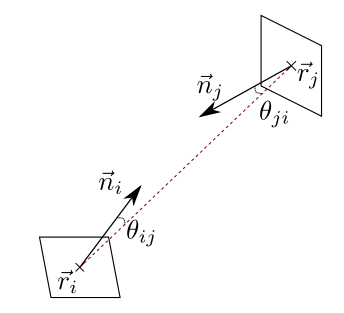
\includegraphics[width = 0.3\linewidth]{PICTURES/FIJ.png}
    \caption{Illustration des notations géométriques introduites à l'Eq \ref{eq:irra}}
    \label{fig:fij_schema}
\end{figure}

La connaissance des radiosités est donc capitale pour les transferts radiatifs.









\subsection{Le modèle des facteurs de vue d'ordre 1}
Les facteurs de vue d'ordre 1 repose sur l'hypothèse d'\textbf{uniformité de la radiosité et de la température sur une surface}. Cette hypothèse permet d'introduire des $\overline{J_i^1} \; [W/m^2]$, et de découpler le terme géométrique $f_{ij}$ de la radiosité dans la formule \ref{def:irra}.  On a alors pour $\forall i$:
\red{partir de l'équation précédente}
\begin{equation}
    G_i(\vec{r_i}) = \sum_{j = 1}^{n} \overline{J_j}^1 f_{ij}(\vec{r_i}) \quad \text{avec } f_{ij}(\vec{r_i}) =\frac{1}{\pi} \int_{A_i} d^2(\vec{r_j})\bigg[\frac{cos(\theta_{ij})cos(\theta_{ji})}{||\vec{r_i}-\vec{r_j}||^2} \chi{(\vec{r_i},\vec{r_j})}\bigg] 
\end{equation}

L'intégration sur la surface $i$ permet enfin d'obtenir une approximation à l'ordre 1 la fraction de radiation quittant la surface $i$ intercepté par la surface $j$ appelée facteur de vue.

\begin{equation}
    \label{fv}
    F_{ij} = \frac{1}{A_i} \int_{A_i} \int_{A_j} d^2(\vec{r_i}) d^2(\vec{r_j})\bigg[\frac{cos(\theta_{ij})cos(\theta_{ji})}{\pi ||\vec{r_i}-\vec{r_j}||^2} \chi(\vec{r_i},\vec{r_j})\bigg] 
\end{equation}


Les hypothèses faites reviennent à considérer un problème d'éclairement entre différentes surface couplées. La connaissance des facteurs de vue permet alors de reformuler l'équation \ref{def:radiosite} pour exprimer les radiosités en fonction de la variable température : 

\begin{equation}
    \overline{J_i^1} = \epsilon_i \sigma \overline{T}^4_i  + \rho_i \sum_{j=1}^{n} \overline{J_j^1} F_{ij}
\end{equation}


On remarque par ailleurs que les facteurs de vue respectent des propriétés physiques fondamentales, à savoir :

\begin{equation}    
    \left\lbrace
    \begin{array}{r c c c  }
    
      \forall i ,\forall j, A_i F_{ij} & = & A_j F_{ji} & \text{(relation de réciprocité)}\\
      \forall i , \sum_{j = 1}^n F_{ij} & = & 1 & \text{(relation de fermeture)}\\ 
      \forall i ,\forall j, F_{ij} & \geq & 0 & \text{(positivité)}
    \end{array}\right.
\end{equation}
\label{def:fv}

Enfin, l'Equation \ref{eq:qr} qui permet de définir le flux radiatif devient :
\begin{equation}
    \forall \vec{r}_i \in \text{Surface}_i,\quad q_i(\vec{r}_i) =  \overline{J}_i^1  -  \sum_{j=1}^{n} \overline{J_j^1} F_{ij} \quad = \quad \epsilon_i \sigma \overline{T}^4_i  - \epsilon_i \sum_{j=1}^{n} \overline{J_j^1} F_{ij}
    \label{eq:nice_qr}
\end{equation}




\input{PARTIES/4_methode_fv}

\section{Amélioration des facteurs de vue d'ordre 1}
\section{Amélioration de la méthode Monte Carlo Ray Tracing}
\subsection{Motivations: les problèmes hyper-sensibles}
L'article de Robert P. Taylor, R.Luck et B. K. Hedge \cite{hypersensitive} met en lumière des problèmes hyper-sensibles, c'est à dire des problèmes pour lesquels une petite erreur dans les facteurs de vue peut engendrer une grande erreur lorsqu'elle est propagée dans l'équation de la chaleur. En effet, leur étude de propagation d'incertitude montre une sensibilité extrême de flux de chaleur avec les facteurs de vue. Dans le cas d'une géométrie pourtant simple d'un parallélépipède traité dans \cite{incro}, une précision de $5$ ~\% sur le flux de chaleur nécéssite une précision de $10^{-4}$ sur les facteurs de vue.
Il devient donc évident qu'une méthode Monte-Carlo naïve doit être complétées par des méthodes complémentaires.

\subsection{Algorithmes de renforcement}
Les résultats obtenus par la méthode de lancer de rayon permettent une bonne approximation des facteurs de vue avec une précision statistique en $\frac{1}{\sqrt{N}}$ caractéristique des méthodes Monte-Carlo. Or une approximation trop grossière peut s'avérer critique. Des méthodes de corrections \cite{renforcement95} qui reposent sur les propriétés géométriques des facteurs de vue permettent d'améliorer la convergence de la matrice vers la matrice théorique. L'enjeu est donc d'utiliser une méthode de correction des facteurs de vue moins coûteuse en temps de calcul qu'une augmentation du nombre de tirages.
\subsubsection{Algorithme naïf}
     
$\begin{bmatrix}
                ... & F_{12} & F_{13}\\
                ... & ... & F_{23} \\
                ... & ... & ... 
        \end{bmatrix}$
        -> réciprocité
        $\begin{bmatrix}
                ... & F_{12} & F_{13}\\
                F_{21} & ... & F_{23} \\
                F_{31} & F_{32} & ... 
        \end{bmatrix}$
        -> fermeture
        $\begin{bmatrix}
                F_{11} & F_{12} & F_{13}\\
                F_{21} & F_{22} & F_{23} \\
                F_{31} & F_{32} & F_{33} 
        \end{bmatrix}$

\subsubsection{Algorithme de Leersum}
\subsubsection{Algorithme des moindres carrés}
\subsection{Stratégie d'échantionnage}

\begin{equation}
    \hat{F_{ij}}^{N_i, N_\theta, N_\varphi, N} =  \sum_{h = 1}^{N_i} \frac{A_{i,h}}{A_i} \sum_{l = 1}^{N_{\theta}} \sum_{m = 1}^{N_{\varphi}} \alpha_{l,m} \hat{F}_{ij}^{h,l,m, N} \quad \text{avec } \hat{F}_{ij}^{h,l,m, N} = \frac{1}{N} \sum_{k = 1}^{N} 1_{A_j}(\vec{r_i}^{(h,l,m,k)}, \vec{\Omega_i}^{(h,l,m,k)}) 
    \label{eq:fv1}
\end{equation}

Un estimateur Monte-Carlo de la variance se construit de la même manière.


Le choix de partionner l'hémisphère en $N_\theta \times N_\varphi$ directions de lancement, motivé par \cite{partition} et mise en place dans \cite{Romain25} permet d'aboutir à une décomposition comme la suivante :


La tâche ici n'est pas d'étudier différentes constructions d'estimateurs. La fonction densité de probalilité choisie apparaît natuellement dans la définition de \ref{eq:MCfij}. On introduit donc $p_X = \frac{cos(X)sin(X)}{\pi}$, associée à la constante de normalisation $ \alpha_{l,m} $ conformément à \cite{Romain25}. Cet échantillonage uniforme sur la surface et sur les angles permet d'avoir une fonction poids associée unitaire. On fait donc $N$ tirages pour $(\vec{r_i}^{(l,m,k)}, \vec{\varphi_i}^{(l,m,k)}, \vec{\theta_i}^{(l,m,k)})$. L'estimateur Monte-Carlo de l'espérance :


des stratégies de stratifications seront discutées ultérièrement et donnent de meilleurs résultats de convergence qu'un échantillonage uniforme sur les deux angles \cite{Romain25}.
avec    $\alpha_{l,m}= \frac{\big(\varphi_{m+1}- \varphi_{m} \big)\big(sin^2(\theta_{l+1})-sin^2(\theta_{l})\big)}{2\pi}$.

\begin{equation}
    F_{ij} = \frac{1}{A_i} \int_{A_i} d^2\vec{r}_i \sum_{l = 1}^{N_{\theta}} \sum_{m = 1}^{N_{\varphi}} \int_{\theta_{l}}^{\theta_{l+1}} \int_{\varphi_{m}}^{\varphi_{m+1}} \bigg[\frac{cos(\theta_i) sin(\theta_i)}{\pi} 1_{A_j}(\vec{r_i}, \vec{\Omega_i})\bigg] d\varphi_i d\theta_i
\label{eq:MCfij}
\end{equation}


\subsubsection{Algorithme de renforcement et relation de fermeture}

L'algorithme de renforcement (en anglais "enforcement algorithm") est une méthode de correction qui permet d'obtenir une matrice de facteurs contrainte par les propriétés physiques de ces derniers. Trois méthodes de correction sont présentées et étudiées dans \cite{renforcement} qui aborde une méthode naïve, la méthode de Leersom, et la méthode de l'optimisation des moindres carrés. Les comparaisons en terme de précision et variance montrent que la dernière est la plus performante, et permet d'obtenir une matrice de facteurs de vue qui approxime le mieux les propriétés physique du problème.

\subsection{Méthode complémentaire: Facteurs de vue d'ordre 2}

La méthode des \textbf{facteurs de vue d'ordre 2} permet d'obtenir une approximation plus précise des facteurs de vue en prenant en compte la première interraction indirecte entre les surfaces. Cette amélioration est très utile lorsque les surfaces sont très grossièrement discrétisées. Elle repose sur l'introduction de facteurs de vue d'ordre 2, $\overline{J^2}$, qui prennent en compte la première interaction indirecte entre les surfaces et qui reposent sur les facteurs de vue d'ordre 1 :  $ \forall i, \quad J_i(\vec{r_i}) = J^1_i(\vec{r_i}) + \overline{J^2}_i - \overline{J^1_i} $. L'article \cite{Romain25} montre de la même manière que pour l'ordre 1 comment obtenir la formulation suivante :
\begin{equation}
    \overline{J^2_i} - \overline{J^1_i} - \rho_i \sum_{j=1}^{n} F_{ij}  \bigg(\overline{J^2_j} - \overline{J^1_j}\bigg) = \rho_i \sum_{j=1}^{n}  F_{ij} \epsilon_j \sigma \overline{T^4_j} + \rho_i \sum_{j = 1}^{n} \rho_j \sum_{k=1}^{n} F_{ijk} \overline{J^1_k} - \rho_i \sum_{j=1}^{n} F_{ij} \overline{J^1_j}
\end{equation}
avec $F_{ijk}$ le facteur de vue d'ordre 2, qui correspond à la fraction de radiation quittant la surface $i$ qui est intercepté par la surface $j$ après une première interraction avec la surface $k$. $F_{ijk} = \sum_{l=1}^{N} \frac{A_{i,l}}{A_i} \int_{A_{i,l}} \frac{1}{A_{i,h}} d^2r_i f_{ijk}(\vec{r_i})$. On construit enfin l'estimateur de Monte-Carlo de l'espérance pour les facteurs de vue d'ordre 2 $\forall \alpha = (h,l,m,l',m')$ :
\begin{equation}
    \hat{F}_{ijk}^{N_i, N_\theta, N_\varphi, N} = \sum_{h=1}^{N_i} \frac{A_{i,h}}{A_i} \sum_{l=1}^{N_\theta} \sum_{m=1}^{N_\varphi} \alpha_{l,m} \sum_{l'=1}^{N_\theta} \sum_{m'=1}^{N_\varphi} \alpha_{l',m'} \hat{F}^{\alpha,N}_{ijk}
\end{equation}
avec, toujours pour des poids unitaires sur les angles :
\begin{equation}
    \hat{F}_{ijk}^{\alpha,N} = \frac{1}{N} \sum_{n=1}^{N} 1_{A_j}\big(\vec{r}_i^{\alpha,n}, \vec{\Omega}_{ij}^{\alpha,n}\big) 1_{A_k} \big(\vec{r}_j^{\alpha,n}(\vec{r_i}, \vec{\Omega}_i), \vec{\Omega}_{jk}^{\alpha,n} \big)
\end{equation} 


D'autres pistes d'amélioration peuvent être empruntées. L'objectif ici est de se concentrer sur les facteurs de vue d'ordre deux. Mais une liste non exhaustive de méthodes complémentaires est faite dans \cite{Romain25}. Elles ont pour but de compenser certaines approximations que peuvent engendrer les facteurs de vue. La méthode de Gebhart \cite{gebhart} permet notamment de s'affranchir du biais introduit par la subdivision des facteurs de vue sur les surfaces. 

\subsection{Gabhart}
\begin{equation}
B_{ij} = F_{ij} \epsilon_j + \sum_{k=1}^n F_{ik} (1 - \epsilon_k) B_{kj}
\end{equation}


\begin{equation}
Q_i = q_i A_i = A_i \epsilon_i \sigma T_i^4 - \sum_{j=1}^nA_j\epsilon_j \sigma T_j^4 B_{ij}
\end{equation}




	\chapter{\texttt{embree2TRUST}}
\section{Introduction}
Le lancer de rayons (\textit{ray tracing}) constitue aujourd'hui une approche numérique largement utilisée dans des domaines scientifiques et industriels variés. Initialement popularisée par la synthèse d'images pour le rendu photoréaliste, cette méthode est désormais employée dans des applications aussi diverses que la simulation optique, le transport de particules ou le transfert radiatif. Malgré la diversité des phénomènes physiques considérés, ces applications reposent sur une problématique géométrique commune : déterminer efficacement les intersections entre un très grand nombre de rayons et une géométrie tridimensionnelle complexe.

Cette problématique a conduit au développement de bibliothèques logicielles spécialisées dans la navigation géométrique et l'accélération des calculs d'intersection. En physique des hautes énergies, le framework \textsc{ROOT} développé au CERN intègre ainsi le module de géométrie \texttt{TGeo}, conçu pour le suivi de trajectoires au sein de détecteurs complexes. Cette infrastructure géométrique a notamment servi de fondation au développement de \textsc{ROBAST}, une bibliothèque de lancer de rayons destinée à la simulation optique des télescopes Cherenkov \cite{Brun1997ROOT,Okumura2016}.

Parallèlement, les progrès réalisés dans le domaine du rendu graphique ont conduit au développement de bibliothèques dédiées à l'accélération des calculs d'intersection rayon--géométrie. Parmi celles-ci, \textsc{Intel Embree} constitue aujourd'hui une référence pour les architectures CPU. Cette bibliothèque fournit des structures d'accélération hiérarchiques (\textit{Bounding Volume Hierarchies}, BVH) ainsi que des algorithmes de parcours fortement optimisés permettant de réduire significativement le coût des calculs géométriques \cite{Wald2014Embree}.

Les performances offertes par ces outils ont conduit à leur adoption dans plusieurs codes scientifiques. Par exemple, le modèle de transfert radiatif tridimensionnel \textsc{DART} s'appuie désormais sur Embree afin d'accélérer les tests d'intersection rayon--triangle lors des simulations de scènes urbaines et forestières complexes \cite{Qi2019HybridScene}. Cette convergence illustre le caractère transversal du lancer de rayons : indépendamment de la physique considérée, la recherche d'intersections constitue une brique algorithmique commune pouvant être mutualisée.

Le code de Monte Carlo Ray Tracing présenté dans ce chapitre s'inscrit dans cette démarche. Il s'appuie sur la bibliothèque Embree pour le traitement géométrique des trajectoires des rayons, tandis que les modèles physiques propres au transfert radiatif sont utilisés pour estimer les facteurs de vue entre les surfaces du domaine.

\section{Principe de fonctinnement}
PRincipe de fonctionnement de \texttt{embree}

\section{Premiers résultats}
Toutes les études réalisées dans cette section reposent sur la même méthodologie. Les facteurs de vue théoriques sont établis à partir de la littérature \cite{Howell} et sont disponibles en Annexe \ref{anx:fv}. 

Afin d’évaluer quantitativement la qualité des matrices de facteurs de vue obtenues par le code de Monte Carlo Ray Tracing, celles-ci sont comparées à une matrice de référence $F^{\mathrm{ref}}$. L’écart est mesuré via une erreur quadratique moyenne relative (Relative Root Mean Square Error, RRMSE), définie à partir de l’erreur relative élémentaire.

Pour chaque coefficient non négligeable de la matrice de référence, l’erreur relative est définie par :

\begin{equation}
\varepsilon_{ij} =
\frac{
F_{ij}^{\mathrm{calc}} - F_{ij}^{\mathrm{ref}}
}{
F_{ij}^{\mathrm{ref}}
}.
\end{equation}

Afin d’éviter les divisions par des valeurs nulles ou numériquement négligeables, seuls les coefficients vérifiant :

\begin{equation}
\left|F_{ij}^{\mathrm{ref}}\right| > \varepsilon_{\mathrm{th}},
\qquad \text{avec } \varepsilon_{\mathrm{th}} = 10^{-15},
\end{equation}

sont retenus dans le calcul. L’ensemble des indices satisfaisant cette condition est noté $\Omega$.

La métrique globale est ensuite définie comme la racine de la moyenne des carrés des erreurs relatives :

\begin{equation}
\mathrm{RRMSE}
=
\sqrt{
\frac{1}{|\Omega|}
\sum_{(i,j)\in \Omega}
\varepsilon_{ij}^{2}
}.
\end{equation}

Cette grandeur fournit une mesure globale, sans dimension, de l’écart entre la matrice calculée et la matrice de référence. Une valeur nulle correspond à une concordance exacte, tandis qu’une augmentation de cette métrique traduit une dégradation progressive de l’accord entre les deux solutions. Cette grandeur est utilisée par la suite pour analyser la convergence et la qualité des résultats en fonction des paramètres de simulation.

\subsection{Simulation MCRT en 3D}

\begin{figure}[H]
\centering

\begin{minipage}{0.45\textwidth}
\centering

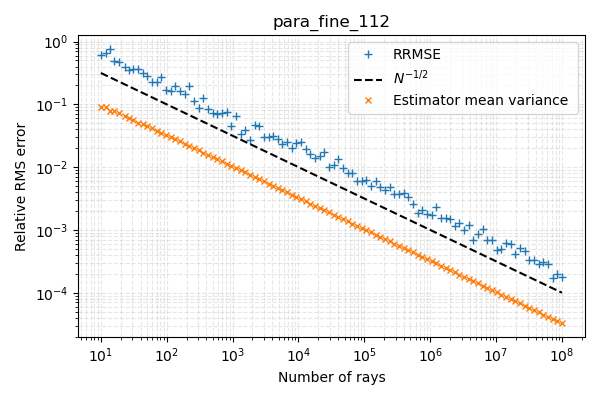
\includegraphics[width = 1\linewidth]{PICTURES/c2/VERIF/rms_convergence_para_fine_112.png}
\small\textbf{(a) Cas d'un parallélépipède}
\end{minipage}
\hfill
\begin{minipage}{0.45\textwidth}
\centering
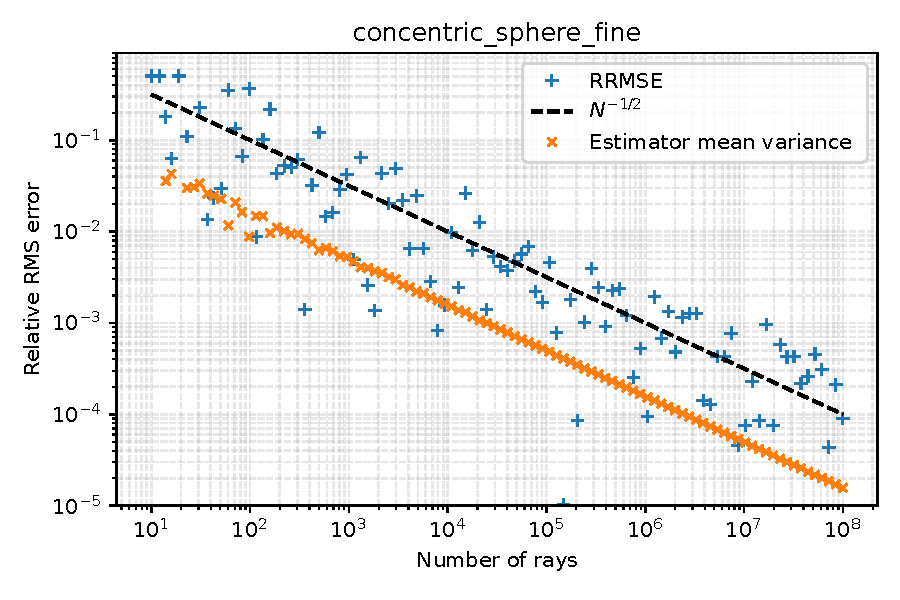
\includegraphics[width = 1\linewidth]{PICTURES/c2/VERIF/convergence_cs_f.pdf}


\small\textbf{(b) Cas de deux sphères concentriques}
\end{minipage}

\caption{Convergence des facteurs de vue pour des géométries en 3D.}
\label{fig:verif3D}

\end{figure}
\subsection{Simulation MCRT avec des géométries 2D}
\label{part:2Dcomp}

\begin{figure}[H]
\centering

\begin{minipage}{0.45\textwidth}
\centering

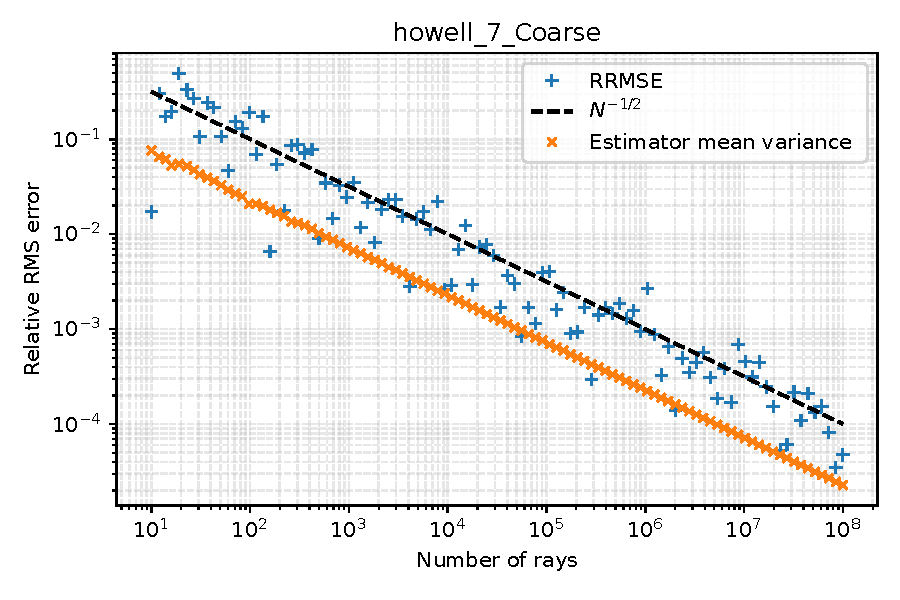
\includegraphics[width = 1\linewidth]{PICTURES/c2/VERIF/convergence_h7.pdf}
\small\textbf{(a) Cas de deux arrêtes adjacentes d'un carré}
\end{minipage}
\hfill
\begin{minipage}{0.45\textwidth}
\centering
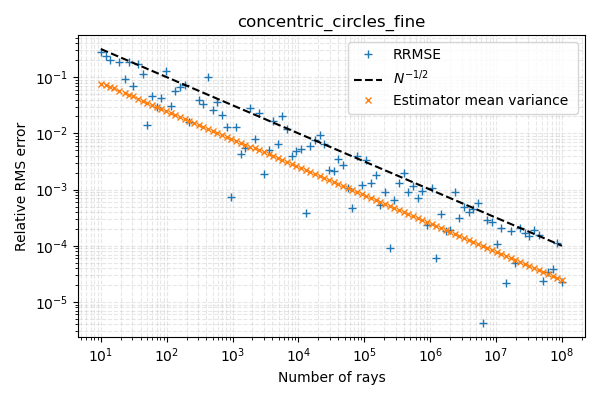
\includegraphics[width = 1\linewidth]{PICTURES/c2/VERIF/convergence_cc_fine.png}


\small\textbf{(b) Cas de deux cercles concentriques}
\end{minipage}

\caption{Convergence des facteurs de vue pour des géométries en 2D.}
\label{fig:verif3D}

\end{figure}







\subsection{Simulation MCRT avec des faces miroires}
\begin{figure}[H]
\centering

\begin{minipage}{0.45\textwidth}
\centering

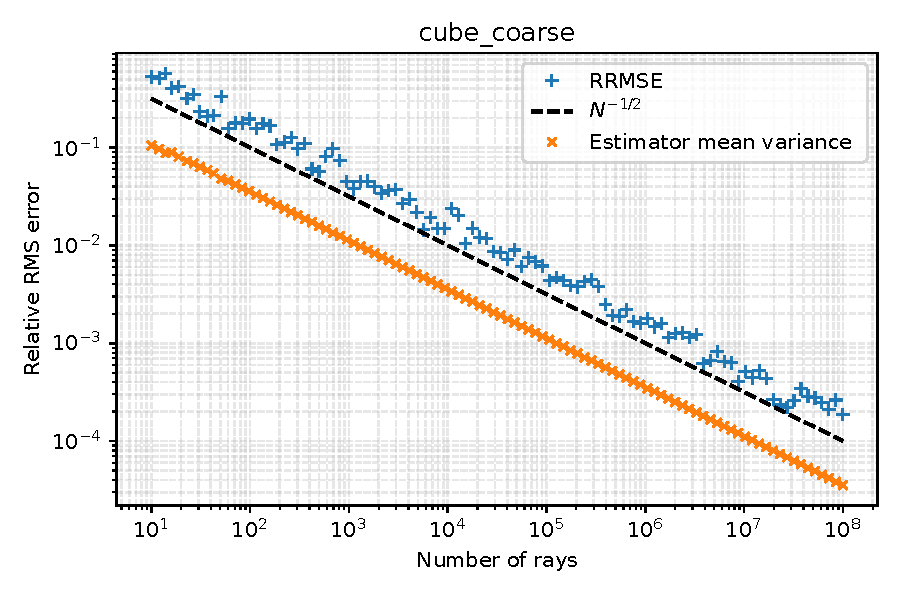
\includegraphics[width = 1\linewidth]{PICTURES/c2/VERIF/convergence_cube_sym_coarse.pdf}
\small\textbf{(a) Cas d'un cube avec une face miroire}
\end{minipage}
\hfill
\begin{minipage}{0.45\textwidth}
\centering
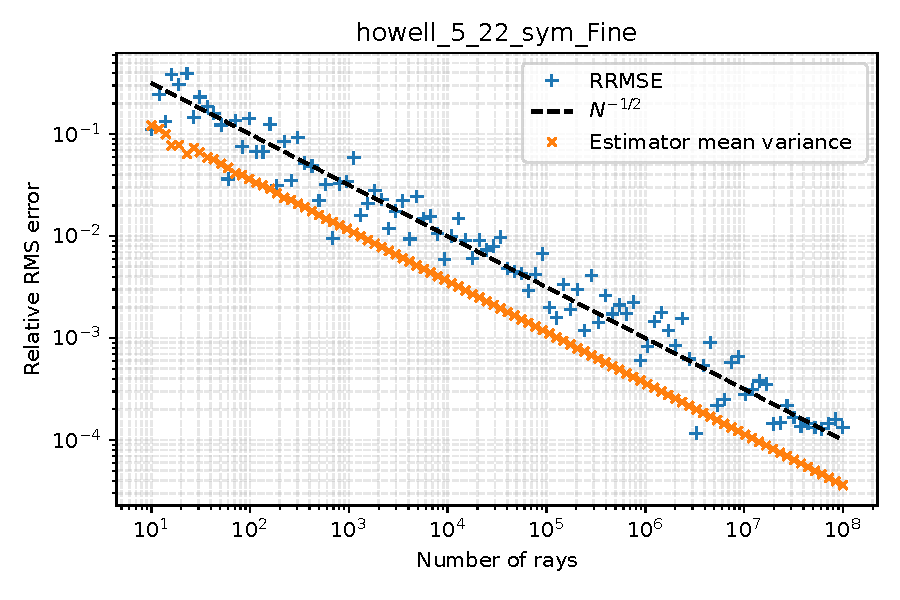
\includegraphics[width = 1\linewidth]{PICTURES/c2/VERIF/convergence_h5_22_sym_Fine.pdf}


\small\textbf{(b) Cas d'une rangée infinie de cercle}
\end{minipage}

\caption{Convergence des facteurs de vue pour des géométries avec faces réflectives.}
\label{fig:verif3Dmiror}

\end{figure}




	
	\chapter{Vérification physique}

\section{Vérification des flux de chaleur}
\label{part:q}
\subsection{Calcul des flux radiatifs}

Une fois les facteurs de vue calculés, ceux-ci sont utilisés pour déterminer les flux radiatifs échangés entre les différentes surfaces. Le calcul repose sur la méthode des radiosités, adaptée dans notre cas d'échanges radiatifs entre surfaces opaques, diffuses et grises \cite{howell}.

On peut reformuler l'Equation \ref{def:radio} pour obtenir le système d'équation suivant:

\begin{equation}
J_i
=
\varepsilon_i \sigma T_i^4
+
(1-\varepsilon_i)
\sum_{j=1}^{N}
F_{ij}J_j,
\label{eq:radiosity}
\end{equation}

où $\varepsilon_i$ est l'émissivité de la surface, $T_i$ sa température, $\sigma$ la constante de Stefan-Boltzmann et $F_{ij}$ le facteur de vue entre les surfaces $i$ et $j$.

En introduisant le vecteur des radiosités $\mathbf{J}$, le vecteur des températures élevées à la puissance quatre $\mathbf{T}^4$ ainsi que la matrice diagonale des émissivités

\begin{equation}
\mathbf{E}
=
\mathrm{diag}(\varepsilon_1,\ldots,\varepsilon_N),
\end{equation}

le système peut être réécrit sous forme matricielle :

\begin{equation}
\left[
\mathbf{I}
-
(\mathbf{I}-\mathbf{E})\mathbf{F}
\right]
\mathbf{J}
=
\mathbf{E}\sigma\mathbf{T}^4.
\label{eq:systeme_radiosite}
\end{equation}

La matrice

\begin{equation}
\mathbf{A}
=
\mathbf{I}
-
(\mathbf{I}-\mathbf{E})\mathbf{F}
\end{equation}

est construite à partir des facteurs de vue et des émissivités. Le système linéaire est ensuite résolu afin de déterminer les radiosités de l'ensemble des surfaces.

Le flux radiatif net quittant chaque surface est finalement obtenu par

\begin{equation}
q_i
=
J_i
-
\sum_{j=1}^{N}
F_{ij}J_j,
\end{equation}

soit, sous forme matricielle,

\begin{equation}
\mathbf{q}
=
(\mathbf{I}-\mathbf{F})\mathbf{J},
\end{equation}

ce qui conduit à l'expression finale

\begin{equation}
\mathbf{q}
=
(\mathbf{I}-\mathbf{F})
\left[
\mathbf{I}
-
(\mathbf{I}-\mathbf{E})\mathbf{F}
\right]^{-1}
\mathbf{E}\sigma\mathbf{T}^4.
\label{eq:q_final}
\end{equation}

Cette formulation montre que les flux radiatifs sont entièrement déterminés par les facteurs de vue, les émissivités des surfaces et leurs températures. Elle constitue l'approche classique retenue pour le calcul des échanges radiatifs en enceinte fermée \cite{howell}.

\subsection{Comparaison avec la littérature}


Exemple 5.5 p210 -> on retrouve le bon flux pour la température calculée, système fermé à $1.10^{-4}$~W/m² près

Exercice 5.22 p 256 -> on retrouve le bon flux pour la température calculée, système fermé à $1.10^{-4}$~W/m² près


\section{Vérification par comparaison avec le code \ttt{pyMCRAD}}
\label{part:pymcrad}
\section{Couplage conduction-rayonnement dans TRUST}


Les chapitres précédents ont permis de vérifier le calcul des facteurs de vue ainsi que le calcul des échanges radiatifs entre surfaces diffuses grises. L'objectif est désormais d'intégrer ce modèle au sein d'un code de calcul thermique afin de simuler le couplage entre la conduction dans les solides et les échanges radiatifs en milieu transparent.

La plateforme \textsc{TRUST} (\textit{TRio\_U Software for Thermal-hydraulics}) \footnote{\url{(https://cea-trust-platform.github.io/}}\cite{saikali2025trust}, développée par le CEA, est un environnement de simulation multiphysique reposant sur une discrétisation par volumes finis. Initialement conçue pour la thermohydraulique, elle permet également de résoudre des problèmes de conduction thermique, de convection et de transferts couplés sur des géométries complexes. Son architecture modulaire facilite l'ajout de nouveaux modèles physiques, ce qui en fait un support adapté au développement d'un modèle de rayonnement thermique en milieu transparent.

Des travaux préliminaires ont été réalisés au CEA autour du couplage conduction-rayonnement à l'aide de la maquette \texttt{python} \texttt{pyMCRAD}, développée par Romain Le Tellier. Cette maquette a permis de démontrer la faisabilité du couplage entre le calcul des facteurs de vue et la résolution thermique. En revanche, elle repose sur des facteurs de vue préalablement connus et reste limitée à des géométries bidimensionnelles simples. L'objectif du présent travail est de lever ces limitations en intégrant directement le calcul des facteurs de vue à partir du maillage utilisé par \textsc{TRUST}, afin de permettre la simulation de géométries tridimensionnelles quelconques.




\section{Problème physique étudié}

Le domaine étudié est constitué de plusieurs solides séparés par un milieu transparent, comme illustré Figure~\ref{fig:domaine}. Les échanges thermiques dans les solides sont gouvernés par la conduction, tandis que les surfaces en contact avec le milieu transparent échangent de l'énergie par rayonnement. Le milieu transparent n'absorbe ni n'émet de rayonnement ; il constitue uniquement le support de propagation des rayons entre les surfaces.

\begin{figure}[H]

\begin{minipage}{0.55\textwidth}
    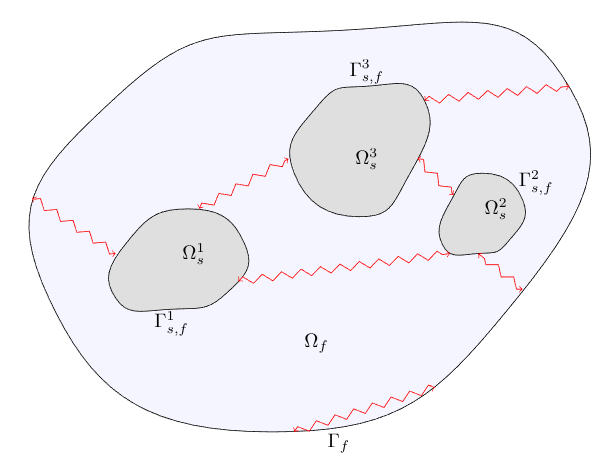
\includegraphics[width=1\linewidth]{PICTURES/domaine.png}
    

    
\end{minipage}
\hfill
\begin{minipage}{0.4\linewidth}
    Notations :
    
    $\Omega_s^i$ les différents domaines solides.
    
    $\Omega_s$ le domaine fluide.
    
    $\Gamma^i_{s,f}$ l'interface entre le solide $i$ et le fluide.
    
    \begin{tikzpicture} 
        \draw[<->, red , decorate, decoration={zigzag, amplitude=2pt}]
        (0, 0) -- (0.67,0);
    \end{tikzpicture} Un symbole pour le couplage.
\end{minipage}
\caption{Schéma typique d’un problème de couplage conduction-rayonnement en milieu transparent}
\label{fig:domaine}
\end{figure}

Dans chaque domaine solide $\Omega_s^i$, la température est obtenue par résolution de l'équation de la chaleur

\begin{equation}
\rho_s^i C_p^i
\frac{\partial T}{\partial t}
=
\nabla\cdot
\left(
\lambda_s^i
\nabla T
\right)
+
\dot q_{\mathrm{vol}}.
\end{equation}

Dans cette étude, le milieu transparent n'intervient pas directement dans le transport radiatif. Lorsque sa résolution thermique est nécessaire, sa température est obtenue à partir de l'équation classique de diffusion

\begin{equation}
\rho_f C_{p,f}
\frac{\partial T}{\partial t}
=
\nabla\cdot
\left(
\lambda_f
\nabla T
\right)
+
\dot q_{\mathrm{vol}}.
\end{equation}

Le couplage entre les domaines solides et le milieu transparent est assuré aux interfaces $\Gamma_{s,f}^i$. La température est supposée continue et le bilan des flux s'écrit

\begin{equation}
\left\{
\begin{aligned}
T_s &= T_f,\\
-\lambda_s\nabla T_s\cdot\mathbf n
&=
-\lambda_f\nabla T_f\cdot\mathbf n
+
q_r,
\end{aligned}
\right.
\end{equation}

où $q_r$ désigne le flux radiatif net calculé à partir des facteurs de vue présentés au chapitre précédent.

Dans le cadre de ce stage, l'étude se limite au couplage entre la conduction dans les solides et les échanges radiatifs de surface à surface. Les simulations sont réalisées sous les hypothèses de surfaces opaques, diffuses grises, d'un milieu transparent et de propriétés thermophysiques constantes.

	
	
	\section{Cas de vérification sur une géométrie bidimensionnelle infinie}

Afin de vérifier le couplage entre le solveur thermique \trust et le module de calcul radiatif développé au cours de ce stage, les résultats obtenus sont comparés à ceux de la maquette de référence \texttt{pyMCRAD}. Cette dernière constitue un cas de validation pertinent puisqu'elle implémente le même modèle physique de conduction-rayonnement en milieu transparent pour des géométries bidimensionnelles.

Le cas considéré représente une rangée infinie de crayons combustibles modélisée par un motif élémentaire de dix crayons. Les conditions de périodicité suivant la direction verticale permettent de reproduire un milieu infini, le motif étant illustré à la Figure~\ref{fig:domaine}. Les facteurs de vue sont cette fois calculés directement à partir du maillage par le module MCRT, puis utilisés dans la résolution thermique sous \trust.

\begin{figure}[H]

\begin{minipage}{0.2\textwidth}
    \centering
    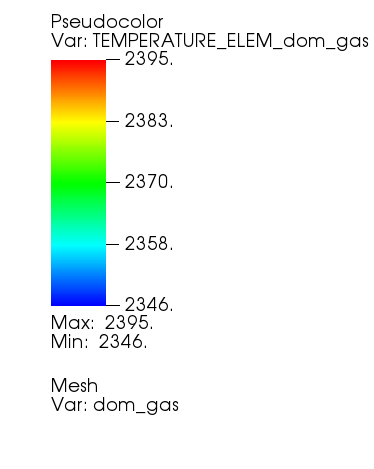
\includegraphics[width=\linewidth]{PICTURES/c5couplage/legend.png}
\end{minipage}
\hfill
\begin{minipage}{0.75\linewidth}
    \centering
    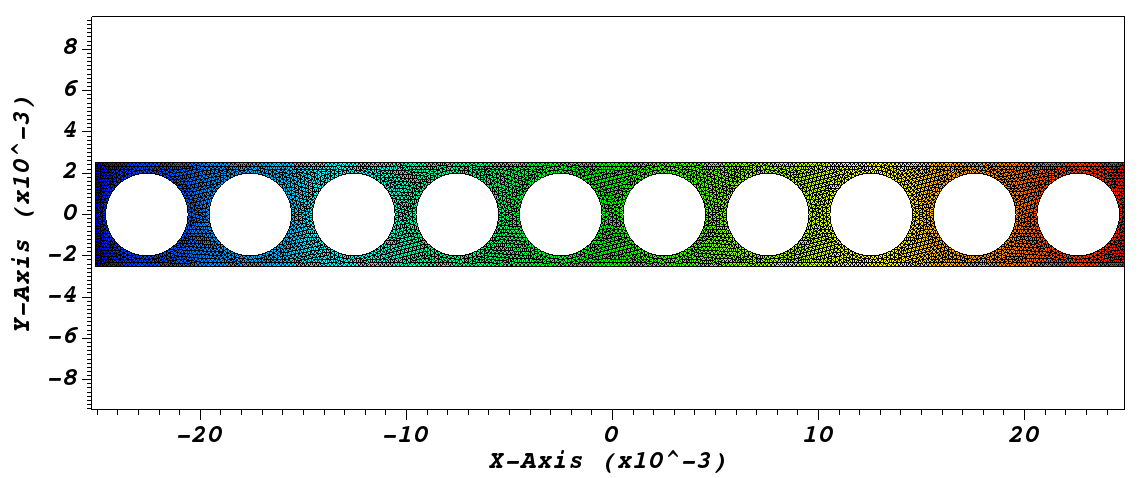
\includegraphics[width=\linewidth]{PICTURES/c5couplage/mesh.png}
\end{minipage}

\caption{Motif élémentaire de dix crayons répété périodiquement suivant les directions $y^+$ et $y^-$.}
\label{fig:domaine}

\end{figure}

La comparaison est réalisée au travers de la conductivité thermique équivalente apparente $K_a$, grandeur classiquement utilisée pour caractériser les transferts thermiques dans les milieux poreux \cite{romain26}. Celle-ci est définie par

\begin{equation}
K_a(T_0)=
\frac{R}{2L_Y\Delta T}
\int_{\Gamma_L\cup\Gamma_R}
\left|\mathbf q\cdot\mathbf n\right|
\,\mathrm dS,
\end{equation}

où $\mathbf q$ désigne le flux thermique total traversant les frontières latérales du domaine.

\begin{figure}[H]
\centering
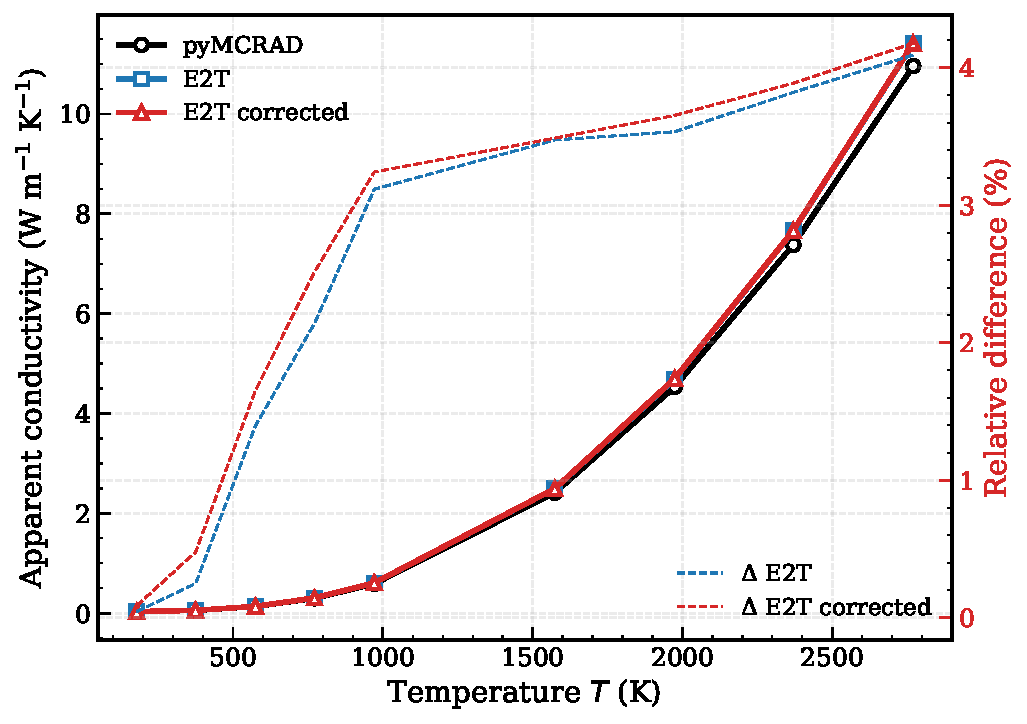
\includegraphics[width=0.9\linewidth]{PICTURES/c5couplage/Ka_vs_T.pdf}
\caption{Comparaison de la conductivité thermique équivalente obtenue avec \textsc{TRUST} et \texttt{pyMCRAD}.}
\label{fig:ka}
\end{figure}

La Figure~\ref{fig:ka} met en évidence un bon accord entre les deux approches sur l'ensemble de la plage de températures étudiée. Les deux modèles reproduisent la même évolution de la conductivité équivalente lorsque la température augmente, ce qui confirme la bonne intégration du calcul radiatif au sein de \textsc{TRUST}.

Les écarts les plus importants apparaissent aux températures les plus élevées. Ce comportement est attendu puisque la contribution du rayonnement devient alors prépondérante, les échanges radiatifs évoluant comme la quatrième puissance de la température. Dans ces conditions, une faible variation des facteurs de vue se traduit directement par une variation plus importante des flux radiatifs.

L'écart maximal observé reste inférieur à 5~\%. Il est principalement attribué aux différences de représentation géométrique entre les deux modèles. Dans le cas présent, les crayons combustibles sont discrétisés par des polygones réguliers de 64 côtés. Comme discuté en Annexe~\ref{annexe:geom}, cette approximation modifie légèrement les facteurs de vue géométriques. Or, l'étude de sensibilité présentée en Section~\ref{part:hypersens} a montré que les flux radiatifs sont particulièrement sensibles à de faibles variations des facteurs de vue. Les écarts observés restent néanmoins compatibles avec cette approximation géométrique et valident le couplage conduction-rayonnement développé dans \textsc{TRUST}.



	
	\chapter{Cas d'application 3D : assemblage de combustible 5x5}
\label{part:c5}

%\section{Motivation de l'étude}
%
Les travaux de \cite{romain25} s'inscrivent dans une approche de calcul à zones couplant conduction et rayonnement, où chaque surface est caractérisée par une unique température moyenne. Cette approche, bien qu'efficace, ne permet pas de rendre compte des écarts de température au sein d'une même surface, écarts pourtant susceptibles d'être significatifs dans des configurations à forte hétérogénéité de puissance.

Cette étude se place dans une perspective différente et complémentaire : il ne s'agit plus de raffiner un modèle à zones, mais d'exploiter directement les capacités de la simulation CFD 3D pour accéder, en plus de la température moyenne $T_{moy}$, aux températures extrémales $T_{max}$ et $T_{min}$ d'une géométrie représentative d'un assemblage de crayons combustible. L'objectif de ce chapitre est ainsi de démontrer la faisabilité d'une étude 3D exigeante sur une telle configuration, de quantifier le biais introduit par la discrétisation géométrique des surfaces sur ces trois grandeurs et d'estimer l'écart entre le point chaud et la température moyenne.

%\section{Mise en place numérique}
%\subsection{Description de la configuration étudiée}

La configuration étudiée est représentative d'un assemblage de crayons combustible, organisé selon un réseau carré de $5\times5$ crayons (soit $25$ crayons au total). Les paramètres géométriques de cet assemblage sont résumés dans le Tableau~\ref{tab:geom_assemblage}, et le domaine de calcul est illustré à la Figure~\ref{fig:domaine}.

\begin{table}[H]
\centering
\begin{tabular}{lcc}
\toprule
Paramètre & Symbole & Valeur \\
\midrule
Nombre de crayons (réseau $5\times5$) & $N_{\mathrm{pins}}$ & $25$ \\
Pas du réseau & $p$ & $16{,}26$~mm \\
Rayon d'un crayon & $R$ & $6{,}26$~mm \\
Hauteur active d'un crayon & $H$ & $250{,}4$~mm \\
\bottomrule
\end{tabular}
\caption{Paramètres géométriques de l'assemblage de crayons combustible.}
\label{tab:geom_assemblage}
\end{table}

\begin{figure}[H]
\centering
\begin{minipage}{0.45\textwidth}
    \centering
    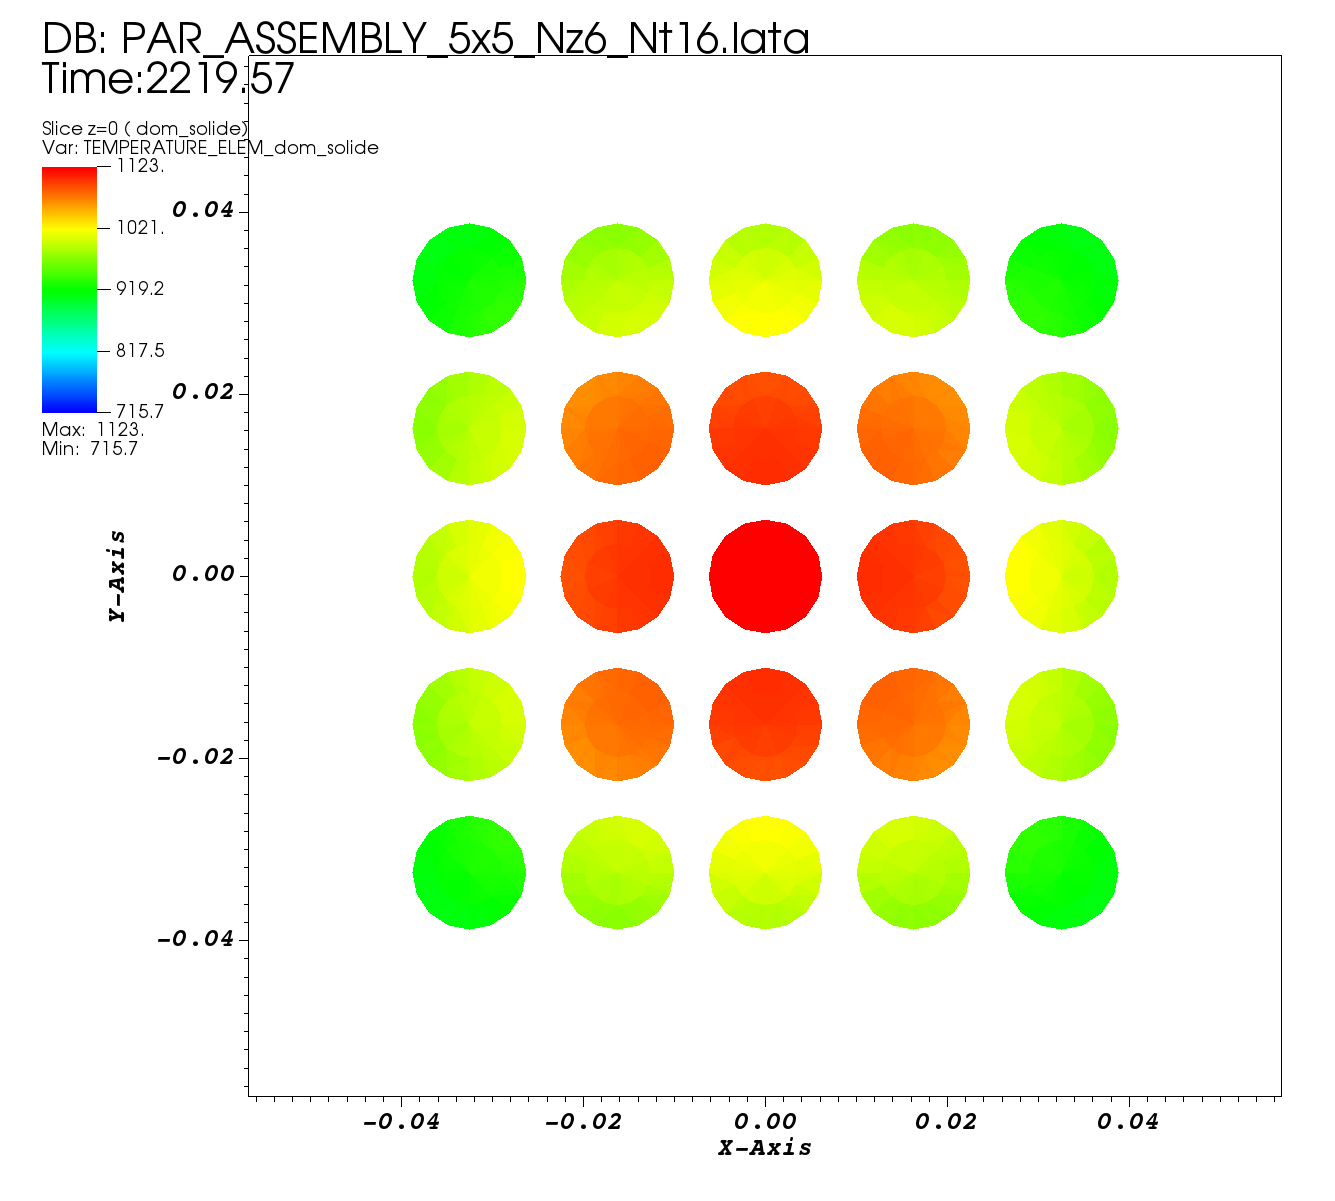
\includegraphics[width=\linewidth]{PICTURES/c5couplage/slicez0.png}
\end{minipage}
\hfill
\begin{minipage}{0.45\textwidth}
    \centering
    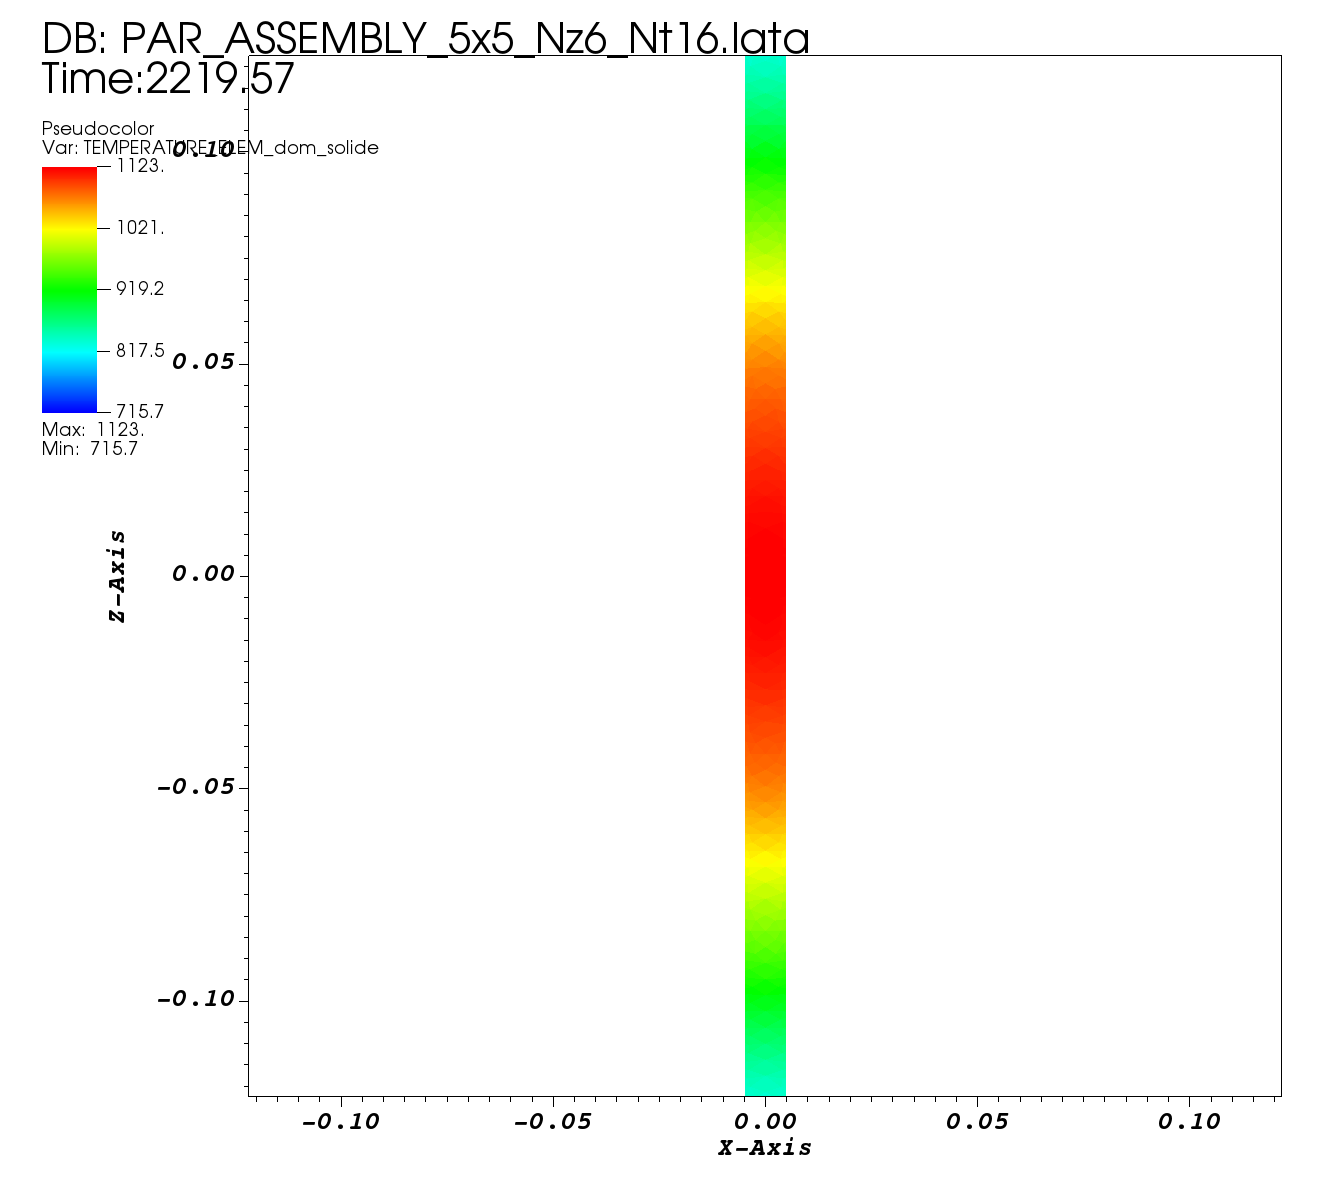
\includegraphics[width=\linewidth]{PICTURES/c5couplage/sliceMid.png}
\end{minipage}
\caption{Plan de coupe en $Z=0$ (gauche) et coupe verticale du crayon central (droite).}
\label{fig:domaine}
\end{figure}

Le combustible et le fluide caloporteur sont caractérisés par les propriétés thermophysiques et radiatives résumées dans le Tableau~\ref{tab:proprietes}. Trois niveaux de puissance volumique sont déposés dans le combustible, modulés selon un profil axial en cosinus caractéristique de la distribution de puissance neutronique le long d'un crayon combustible ; aucune source de puissance n'est imposée dans le fluide. Ces trois cas, résumés dans le Tableau~\ref{tab:puissances}, correspondent à des températures moyennes croissantes du crayon central, permettant d'étudier l'effet de la discrétisation sur une gamme de régimes thermiques représentative. Le fluide est par ailleurs traité sous l'hypothèse de Boussinesq, avec une gravité orientée selon $-\vec{z}$. Une température de paroi $T_{\mathrm{paroi}} = 600$~K est imposée en périphérie du domaine.

\begin{table}[H]
\centering
\begin{tabular}{ccc}
\toprule
Cas & Puissance volumique~[$\mathrm{MW/m^3}$] & $T_{\mathrm{moy}}$ crayon central~[K] \\
\midrule
1 & $3$  & $1013$ \\
2 & $4$  & $1080$ \\
3 & $45$ & $2089$ \\
\bottomrule
\end{tabular}
\caption{Niveaux de puissance volumique étudiés et température moyenne résultante du crayon central.}
\label{tab:puissances}
\end{table}

\begin{table}[H]
\centering
\begin{tabular}{lccc}
\toprule
Propriété & Symbole & Combustible & Fluide \\
\midrule
Masse volumique & $\rho$~[$\mathrm{kg/m^3}$] & $10\,110$ & $6{,}754\times10^{-5}$ \\
Conductivité thermique & $\lambda$~[$\mathrm{W/(m.K)}$] & $10$ & $0{,}01$ \\
Capacité calorifique & $C_p$~[$\mathrm{J/(kg.K)}$] & $350$ & $1141{,}1$ \\
Viscosité dynamique & $\mu$~[$\mathrm{Pa.s}$] & -- & $4{,}153\times10^{-5}$ \\
Coefficient de dilatation thermique & $\beta_{\mathrm{th}}$~[$\mathrm{K^{-1}}$] & -- & $10^{-3}$ \\
Émissivité & $\epsilon$ & $1$ & -- \\
\bottomrule
\end{tabular}
\caption{Propriétés thermophysiques et radiatives du combustible et du fluide caloporteur.}
\label{tab:proprietes}
\end{table}

\subsection{Maillage}

Le maillage surfacique des crayons est généré à l'aide de l'algorithme \texttt{MG-CADSurf} de la plateforme \textsc{Salome}, avec une taille de maille cible comprise entre $2$~mm et $10$~mm. Ce maillage de surface constitue le support du calcul des facteurs de vue par lancer de rayons. Le maillage volumique du domaine fluide, nécessaire à la résolution du problème thermohydraulique dans TRUST, est ensuite généré à partir de ce maillage surfacique à l'aide de l'algorithme tétraédrique \texttt{MG-Tetra}, et comporte environ $1{,}2$ million d'éléments. La Figure~\ref{fig:mesh} présente une coupe horizontale et une coupe verticale de ce maillage.

\begin{figure}[H]
\centering
\begin{minipage}{0.45\textwidth}
    \centering
    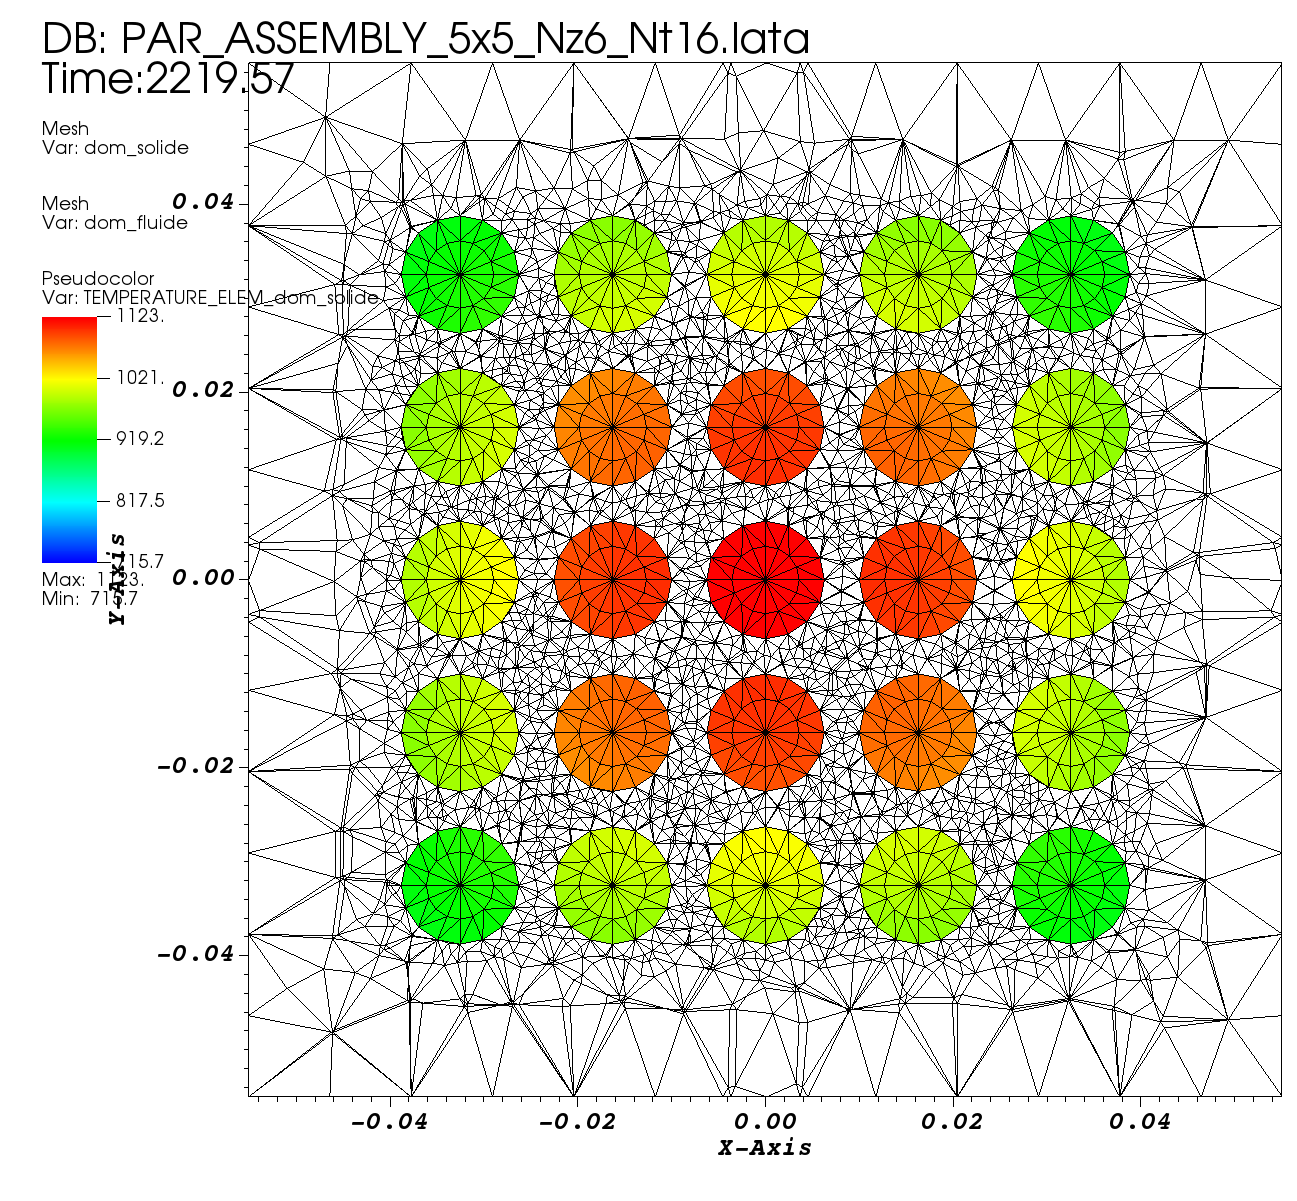
\includegraphics[width=\linewidth]{PICTURES/c5couplage/mesh_horizontal.png}
\end{minipage}
\hfill
\begin{minipage}{0.45\textwidth}
    \centering
    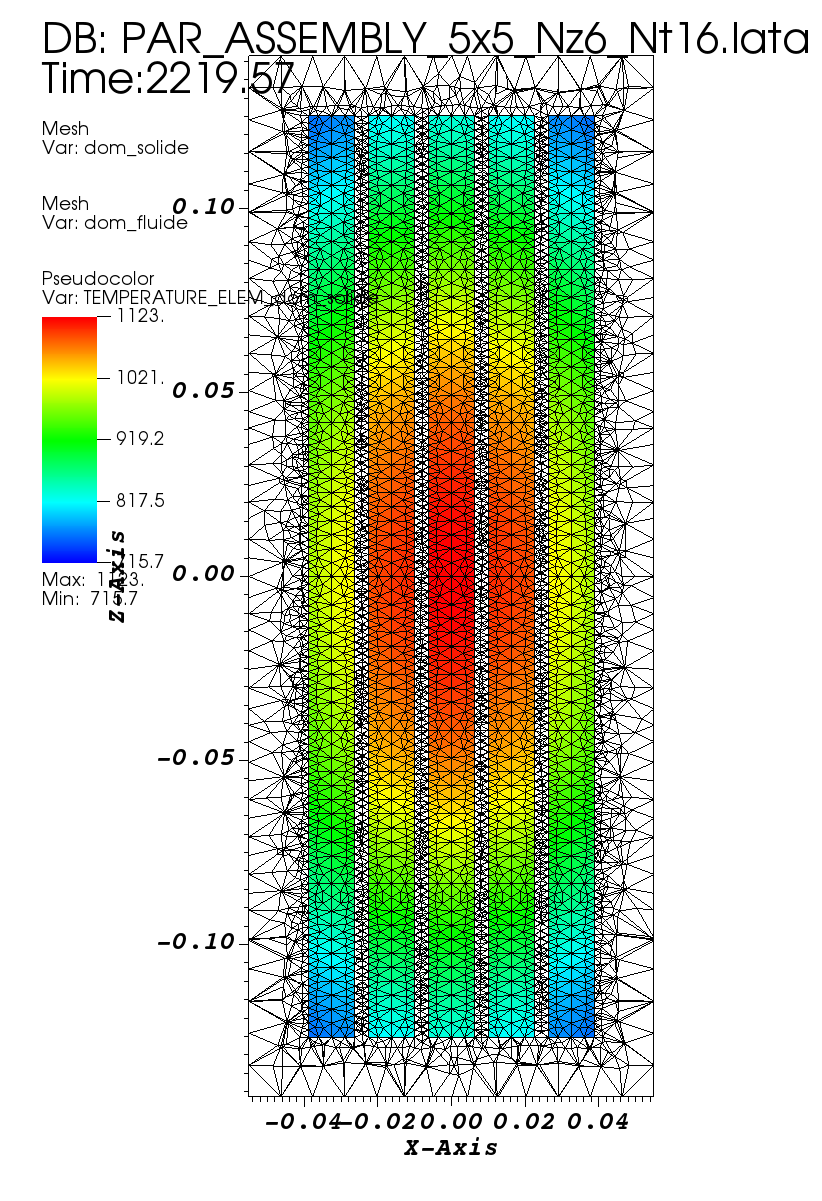
\includegraphics[width=\linewidth]{PICTURES/c5couplage/mesh_vertical.png}
\end{minipage}
\caption{Coupe horizontale en $Z=0$ (gauche) et coupe verticale (droite) du maillage volumique.}
\label{fig:mesh}
\end{figure}

Afin d'étudier l'effet de la discrétisation géométrique sur les résultats, la surface de chaque crayon est en outre discrétisée, pour les besoins du calcul radiatif, selon $N_\theta$ secteurs angulaires et $N_z$ tranches axiales, formant ainsi $N_\theta \times N_z$ sous-surfaces élémentaires par crayon. Le nombre de secteurs angulaires est fixé à $N_\theta = 16$ pour l'ensemble de cette étude. Le nombre de tranches axiales $N_z$, seul paramètre variable, est balayé sur la plage résumée dans le Tableau~\ref{tab:nz_values}, afin de quantifier le biais introduit par l'hypothèse de radiosité uniforme.

\begin{table}[H]
\centering
\begin{tabular}{lc}
\toprule
Paramètre & Valeurs testées \\
\midrule
$N_z$ & $2, 4, 6, \dots, 20$ \\
\bottomrule
\end{tabular}
\caption{Valeurs du nombre de tranches axiales $N_z$ étudiées.}
\label{tab:nz_values}
\end{table}


\subsection{Stratégie de résolution numérique}

Le problème thermohydraulique couplé est résolu dans \trust par une méthode de volumes finis. Bien que l'objectif de cette étude soit d'obtenir l'état stationnaire du système, \trust résout ce problème par une approche de marche en temps : le schéma numérique fait converger la solution vers un point fixe stationnaire par intégration temporelle successive, plutôt que par une résolution directe du problème stationnaire.

Le schéma retenu est un schéma d'Euler implicite, dont le pas de temps $dt$ est piloté automatiquement entre les bornes $dt_{\mathrm{min}}$ et $dt_{\mathrm{max}}$ par un facteur de sécurité \texttt{facsec}. Ce facteur ajuste le pas de temps à chaque itération en fonction de la vitesse de convergence du solveur implicite, permettant d'accélérer la marche en temps tant que la convergence du système linéaire reste satisfaisante. Les principaux paramètres du schéma sont résumés dans le Tableau~\ref{tab:solveur}.

\begin{table}[H]
\centering
\begin{tabular}{lcc}
\toprule
Paramètre & Symbole/mot-clé & Valeur \\
\midrule
Pas de temps minimal & $dt_{\mathrm{min}}$ & $10^{-3}$~s \\
Pas de temps maximal & $dt_{\mathrm{max}}$ & $10^{3}$~s \\
Facteur de sécurité & \texttt{facsec} & $10^{7}$ -- $10^{8}$ \\
Facteur de sécurité maximal & \texttt{facsec\_max} & $10^{8}$ -- $10^{9}$ \\
Seuil de convergence (solveur linéaire) & -- & $10^{-1}$ \\
Seuil de convergence (schéma implicite) & -- & $10^{-1}$ \\
Seuil de stationnarité & \texttt{seuil\_statio} & $10^{-5}$ \\
\bottomrule
\end{tabular}
\caption{Paramètres du schéma temporel implicite utilisé pour la convergence vers l'état stationnaire.}
\label{tab:solveur}
\end{table}

La valeur de \texttt{facsec} retenue, très supérieure à l'unité, illustre bien la nature de cette stratégie : le pas de temps n'est plus piloté par un critère de précision physique de la dynamique transitoire, mais uniquement par la vitesse à laquelle le solveur implicite parvient à converger à chaque itération. Cette approche revient ainsi à utiliser l'intégration temporelle comme un simple outil numérique permettant d'atteindre efficacement l'état stationnaire recherché, sans chercher à représenter fidèlement une éventuelle dynamique transitoire réelle du système. Le calcul est considéré comme convergé lorsque l'évolution de la solution entre deux pas de temps successifs devient inférieure au seuil de stationnarité \texttt{seuil\_statio}.

%\section{Résultats}
%\subsection{Vérifications préliminaires}

Avant d'exploiter les résultats de température issus des simulations, deux vérifications préliminaires ont été menées afin de s'assurer de la cohérence physique du montage numérique.

La première concerne le profil de puissance imposé dans le combustible. La puissance volumique déposée devant suivre un profil axial en cosinus, représentatif de la distribution de puissance neutronique le long d'un crayon, le profil de température visible sur la Figure \ref{fig:profil} montre une bonne adéquation des résultats de la simulation avec les attentes.

\begin{figure}[H]
\centering
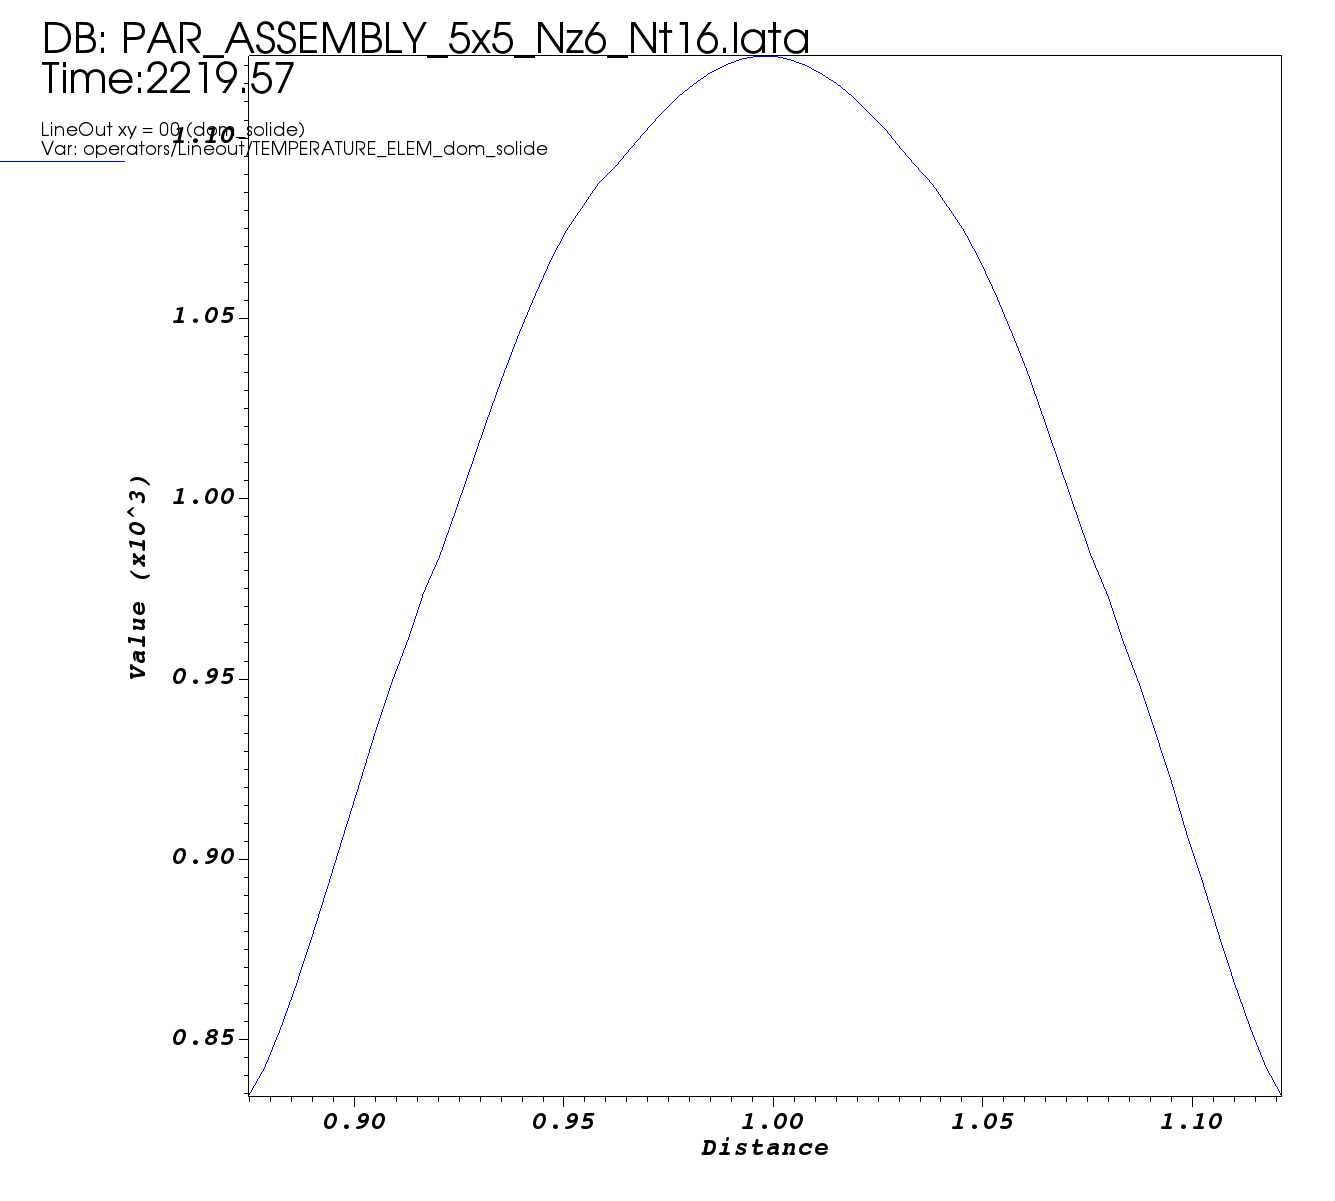
\includegraphics[width=0.6\linewidth]{PICTURES/c5couplage/lineout.png}
\caption{Profil axial de température au centre du crayon central.}
\label{fig:profil}
\end{figure}
La seconde vérification porte sur la conservation globale de l'énergie au sein du système. En régime stationnaire, la puissance totale déposée dans le combustible doit être intégralement évacuée par les mécanismes de transfert thermique du domaine, à savoir la conduction vers la paroi et la convection au sein du fluide caloporteur. Le bilan global de puissance s'écrit ainsi :

\begin{equation}
    P_{\mathrm{volumique}} = P_{\mathrm{sortant}}
    \label{eq:bilan_puissance}
\end{equation}

où $P_{\mathrm{déposée}}$ désigne la puissance volumique totale injectée dans le combustible, et $P_{\mathrm{sortant}} = P_{\mathrm{rad}} + P_{\mathrm{diffusion}}$ les puissances évacuées par les parois du domaine. Cette égalité a été vérifiée sur la plupart des cas étudiés, avec un écart relatif entre la dizaine de $pcm$ au $\%$, confirmant même dans le pire des cas la cohérence du bilan thermique global de la simulation.

\subsection{Conséquence de l'hypothèse de radiosité uniforme}
\begin{figure}[H]
\centering
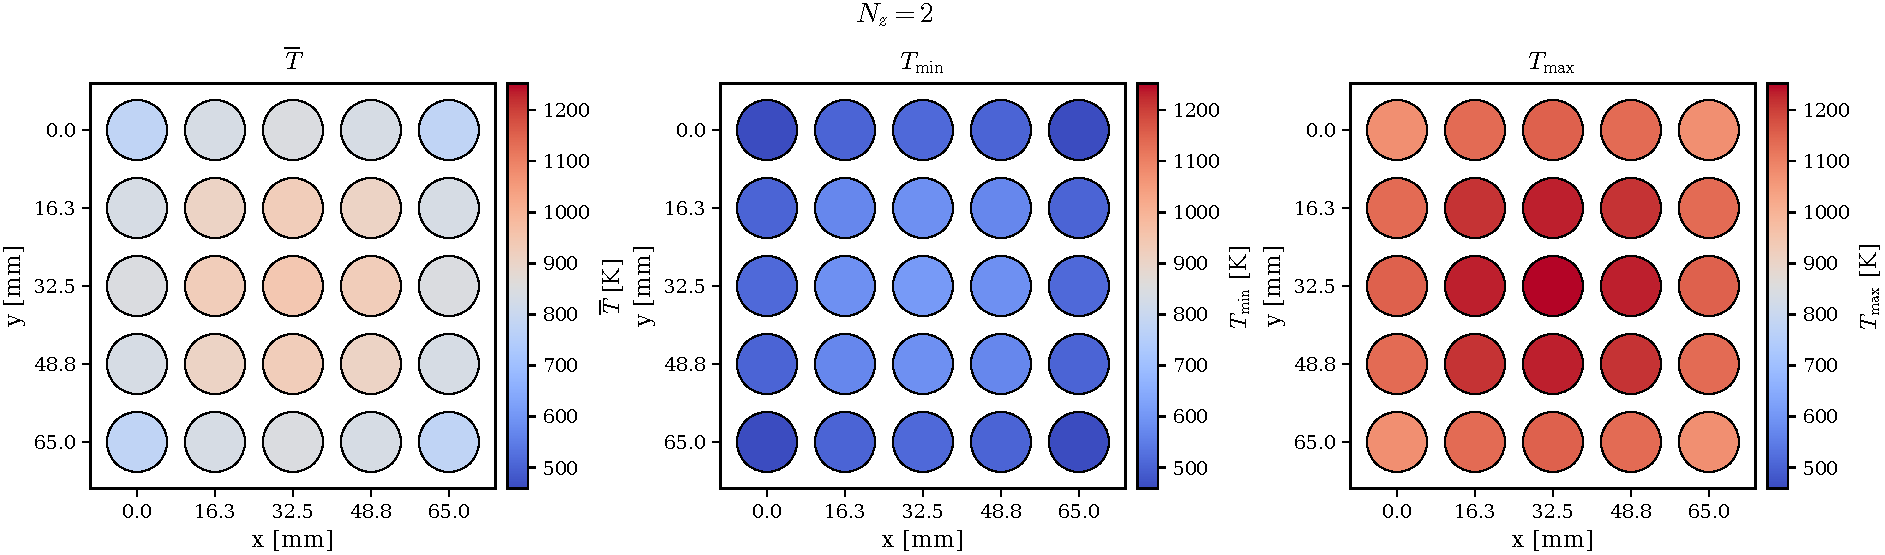
\includegraphics[width=0.8\linewidth]{PICTURES/c5couplage/T925/assembly_2.pdf}
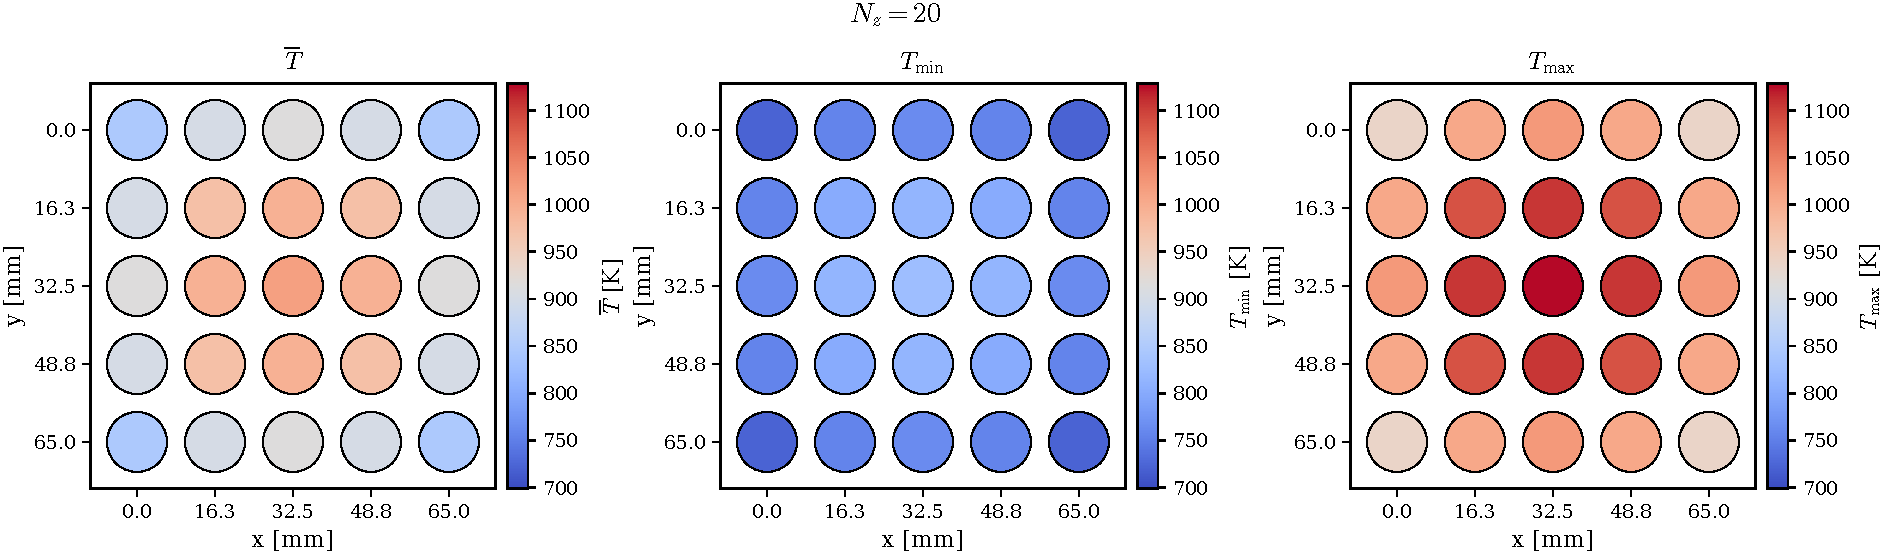
\includegraphics[width=0.8\linewidth]{PICTURES/c5couplage/T925/assembly_20.pdf}
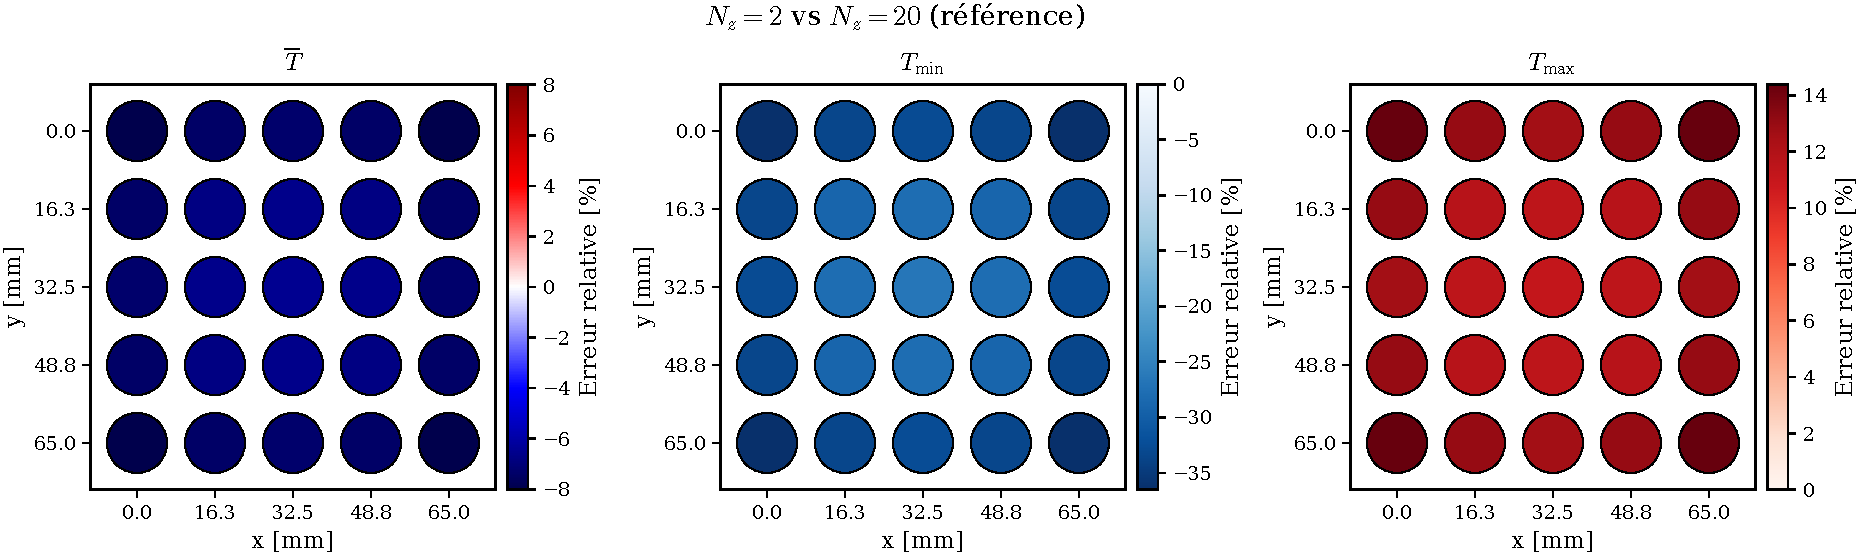
\includegraphics[width=0.8\linewidth]{PICTURES/c5couplage/T925/assembly_diff_2_vs_20.pdf}

 \caption{Températures minimum, maximum et moyenne dans le cas $\overline{T}=925.7$~K}
 \label{fig:temperature3MW}
\end{figure}



\begin{figure}[H]
\centering
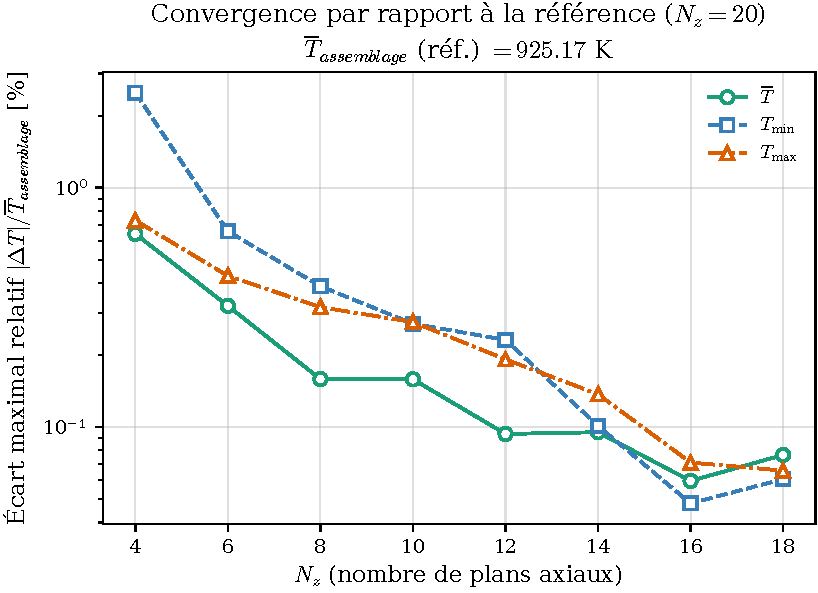
\includegraphics[width=0.7\linewidth]{PICTURES/c5couplage/T925/convergence_relative_vs_20.pdf}

 \caption{Convergence relative des températures dans le cas $\overline{T}=925.7$~K}
 \label{fig:convergence3MW}
\end{figure}




\begin{figure}[H]
\centering
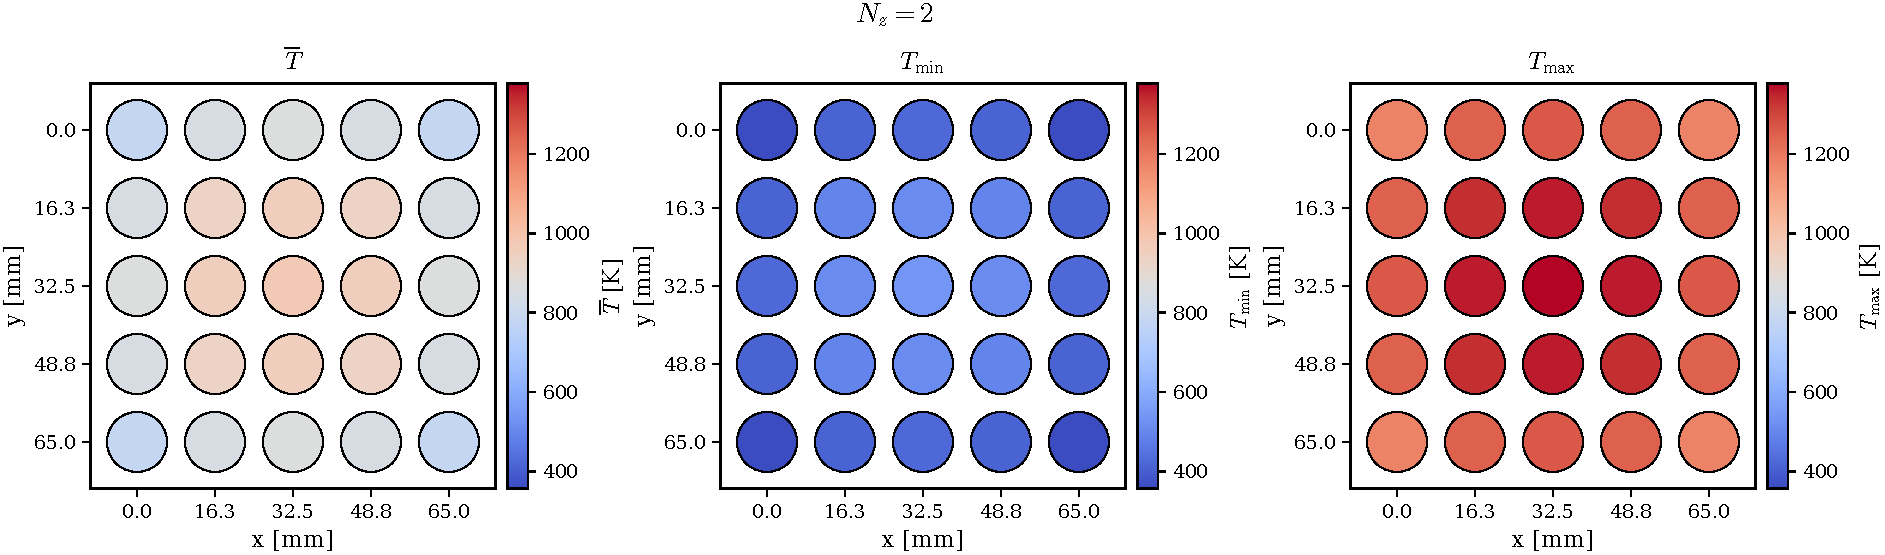
\includegraphics[width=0.8\linewidth]{PICTURES/c5couplage/T1000/assembly_2.pdf}
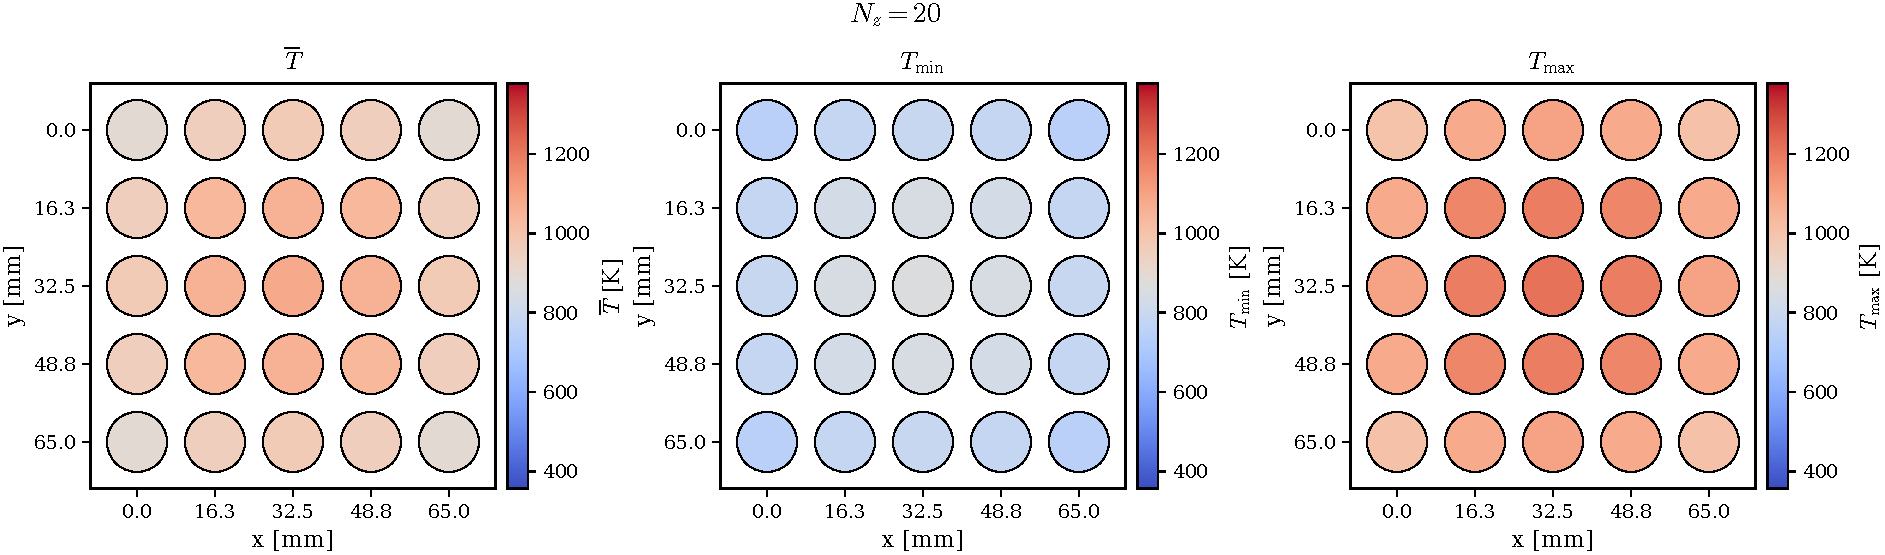
\includegraphics[width=0.8\linewidth]{PICTURES/c5couplage/T1000/assembly_20.pdf}
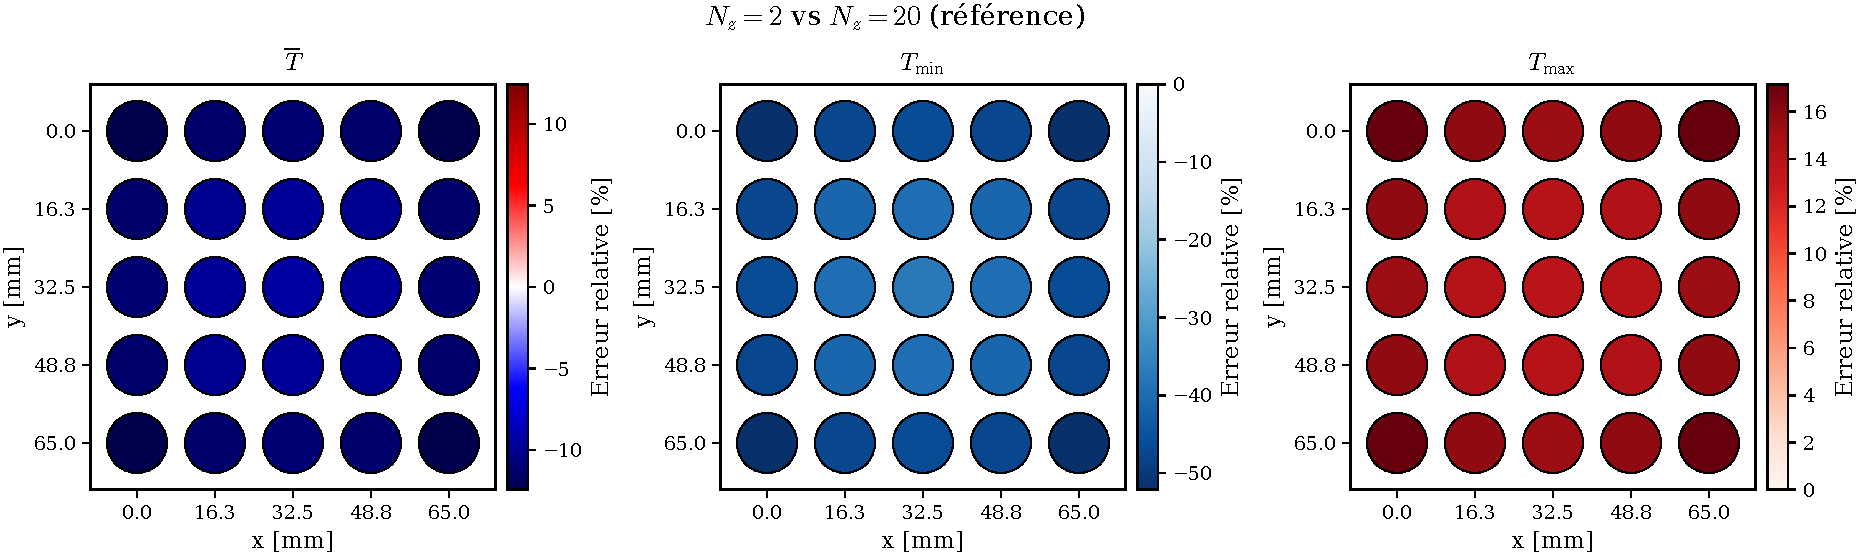
\includegraphics[width=0.8\linewidth]{PICTURES/c5couplage/T1000/assembly_diff_2_vs_20.pdf}

 \caption{Températures minimum, maximum et moyenne dans le cas $\overline{T}=981.4$~K}
 \label{fig:temperature4MW}
\end{figure}



\begin{figure}[H]
\centering
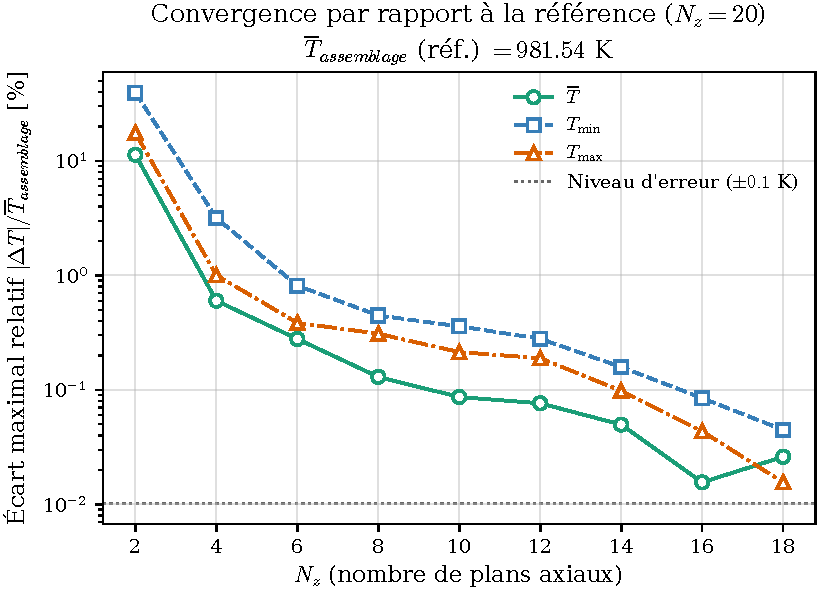
\includegraphics[width=0.7\linewidth]{PICTURES/c5couplage/T1000/convergence_relative_vs_20.pdf}

 \caption{Convergence relative des températures dans le cas $\overline{T}=981.4$~K}
 \label{fig:convergence4MW}
\end{figure}


\subsection{Etude de l'écart entre le point chaud et la température moyenne}
Le Tableau~\ref{tab:tmoy_tmax} rassemble, pour les trois niveaux de puissance étudiés, la température moyenne $T_{\mathrm{moy}}$ et la température maximale $T_{\mathrm{max}}$ obtenues sur le crayon central. On observe que l'écart entre $T_{\mathrm{max}}$ et $T_{\mathrm{moy}}$ croît avec le niveau de puissance déposée, aussi bien en valeur absolue qu'en proportion de la température moyenne. L'intérêt de ce résultat ne réside cependant pas dans ces trois seules valeurs, dont le nombre reste insuffisant pour en tirer une conclusion générale, mais dans la démarche qu'elles illustrent : la capacité à quantifier, à partir d'une simulation CFD 3D complète, l'écart entre température moyenne et température de point chaud pour une configuration donnée. Une telle relation, une fois établie sur un nombre suffisant de cas, ouvrirait la voie à l'estimation de la température de point chaud d'un système à partir de sa seule température moyenne, cette dernière étant directement accessible par des modèles à zones plus simples et bien moins coûteux en temps de calcul que la simulation CFD 3D complète.

\begin{table}[H]
\centering
\begin{tabular}{ccccc}
\toprule
Cas & Puissance volumique~[$\mathrm{MW/m^3}$] & $T_{\mathrm{moy}}$~[K] & $T_{\mathrm{max}}$~[K] & Écart relatif $\frac{T_{\mathrm{max}} - T_{\mathrm{moy}}}{T_{\mathrm{moy}}}$ \\
\midrule
1 & $3$  & $925{,}2$ & $1127$ & \red{...} \\
2 & $4$  & $981{,}5$ & $1211$ & \red{...} \\
3 & $45$ & $1817$    & $2475$ & \red{...} \\
\bottomrule
\end{tabular}
\caption{Températures moyenne et maximale du crayon central pour les trois niveaux de puissance étudiés.}
\label{tab:tmoy_tmax}
\end{table}



\subsection{Conclusion}

\section{Motivation de l'étude}

Les travaux de \cite{romain25} s'inscrivent dans une approche de calcul à zones couplant conduction et rayonnement, où chaque surface est caractérisée par une unique température moyenne. Cette approche, bien qu'efficace, ne permet pas de rendre compte des écarts de température au sein d'une même surface, écarts pourtant susceptibles d'être significatifs dans des configurations à forte hétérogénéité de puissance.

Cette étude se place dans une perspective différente et complémentaire : il ne s'agit plus de raffiner un modèle à zones, mais d'exploiter directement les capacités de la simulation CFD 3D pour accéder, en plus de la température moyenne $T_{\mathrm{moy}}$, aux températures extrémales $T_{\mathrm{max}}$ et $T_{\mathrm{min}}$ d'une géométrie représentative d'un assemblage de crayons combustible. L'objectif de ce chapitre est ainsi de \textbf{démontrer la faisabilité d'une étude 3D exigeante}, \textbf{de quantifier le biais de convergence} de la disctétisation des faces radiatives introduit par les hypothèses du modèle rayonnement en milieu transparent et d'étudier \textbf{l'écart entre le point chaud de  l'assemblage et sa température moyenne}.


\section{Mise en place numérique}

\subsection{Description de la configuration étudiée}

La configuration étudiée est représentative d'un assemblage de crayons combustible, organisé selon un réseau carré de $5\times5$ crayons. Les paramètres géométriques de cet assemblage sont résumés dans le Tableau~\ref{tab:geom_assemblage}, et le domaine de calcul est illustré à la Figure~\ref{fig:domaine}.

\begin{table}[H]
\centering
\renewcommand{\arraystretch}{1.0}
\begin{tabular}{lcc}
\toprule
Paramètre & Symbole & Valeur \\
\midrule
Nombre de crayons (réseau $5\times5$) & $N_{\mathrm{pins}}$ & $25$ \\
Pas du réseau (centre à centre)& $p$ & $16{,}26$~mm \\
Rayon d'un crayon & $R$ & $6{,}26$~mm \\
Hauteur active d'un crayon & $H$ & $250{,}4$~mm \\
\bottomrule
\end{tabular}
\caption{Paramètres géométriques de l'assemblage de crayons combustible.}
\label{tab:geom_assemblage}
\end{table}

\begin{figure}[H]
\centering
\begin{minipage}{0.45\textwidth}
    \centering
    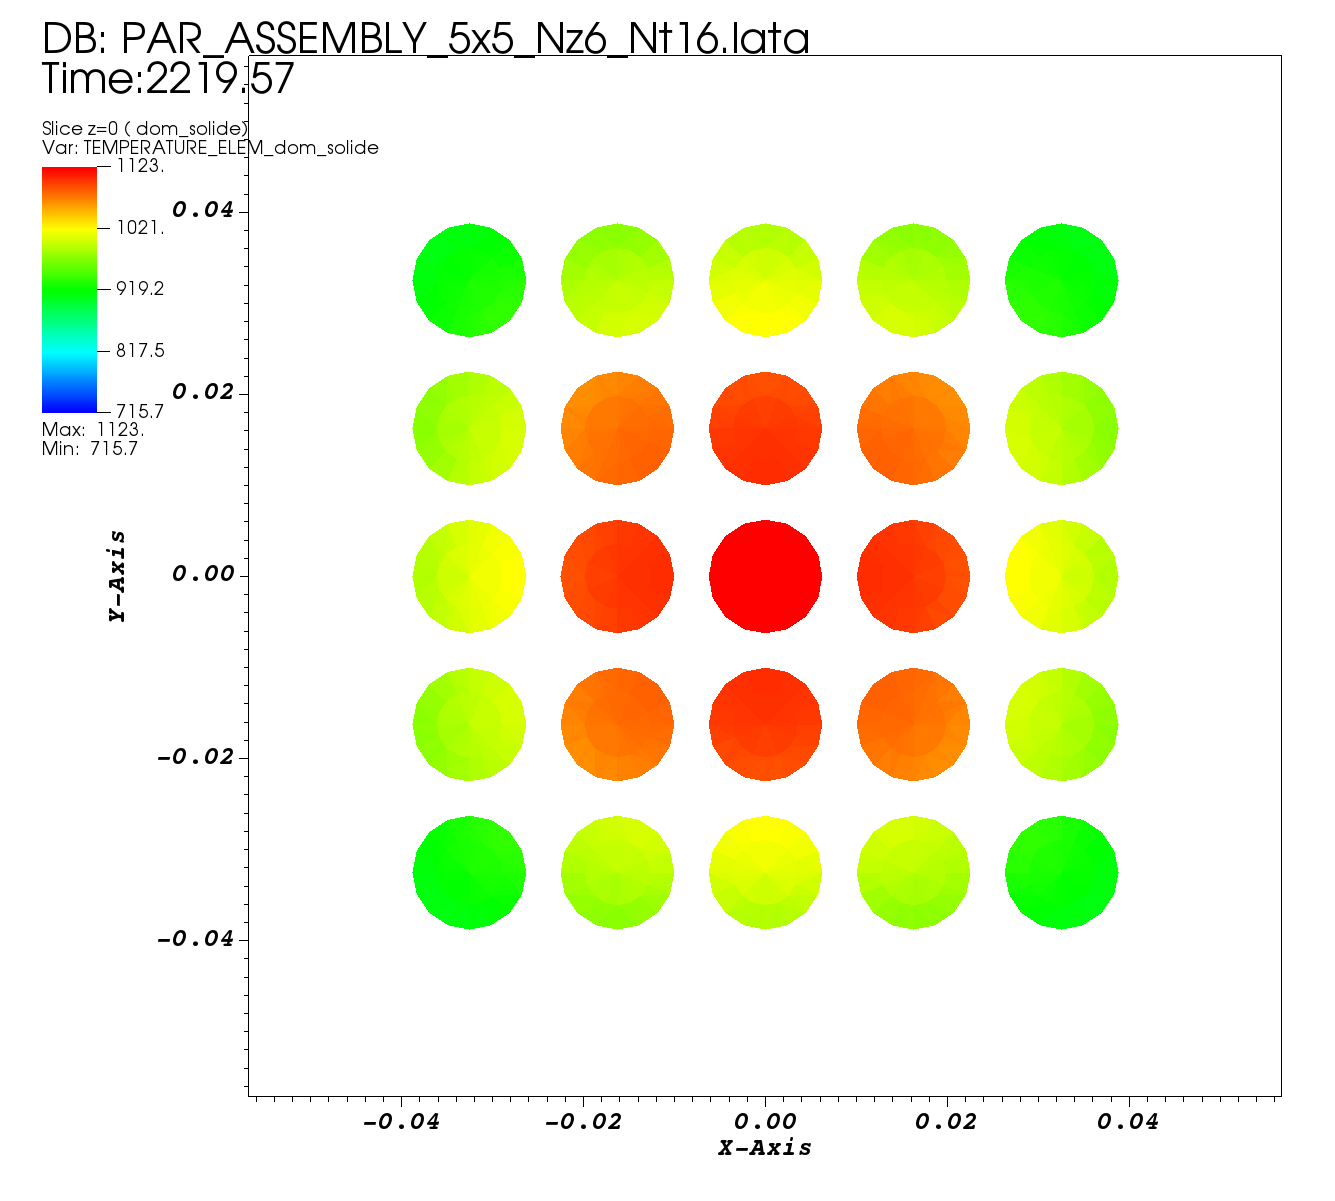
\includegraphics[width=\linewidth]{PICTURES/c5couplage/slicez0.png}
\end{minipage}
\hfill
\begin{minipage}{0.45\textwidth}
    \centering
    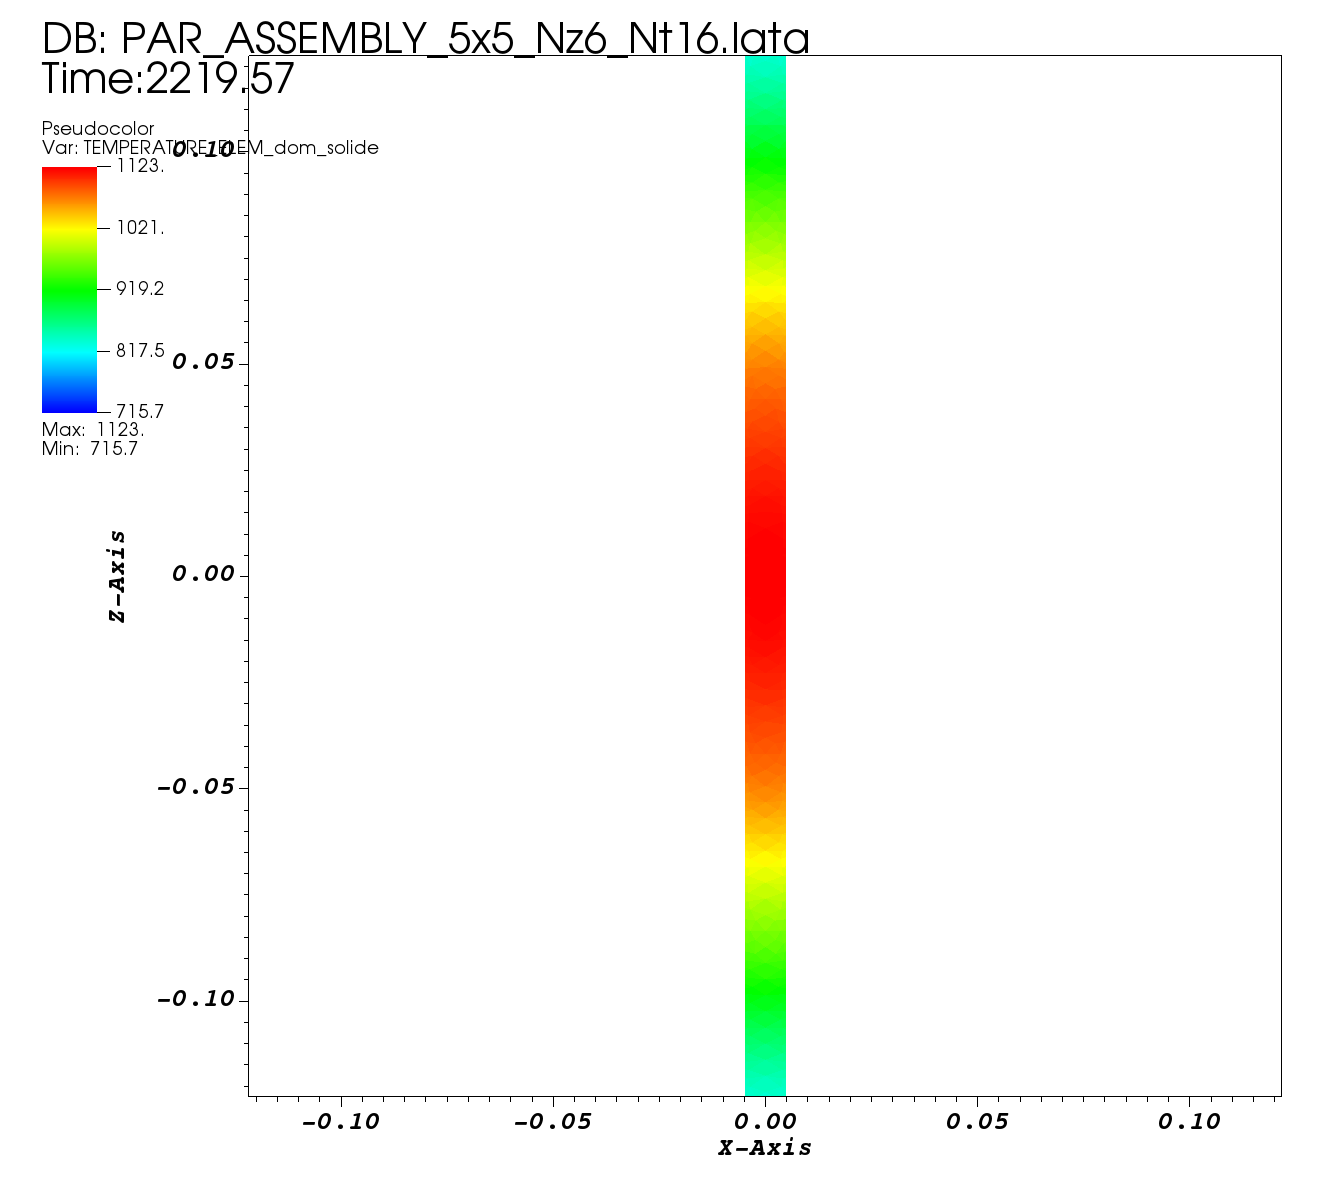
\includegraphics[width=\linewidth]{PICTURES/c5couplage/sliceMid.png}
\end{minipage}
\caption{Plan de coupe en $Z=0$ (gauche) et coupe verticale du crayon central (droite).}
\label{fig:domaine}
\end{figure}

Le combustible et le fluide caloporteur sont caractérisés par les propriétés thermophysiques et radiatives résumées dans le Tableau~\ref{tab:proprietes}. Plusieurs niveaux de puissance volumique sont déposés dans le combustible, modulés selon un profil axial en cosinus caractéristique de la distribution de puissance neutronique le long d'un crayon combustible ; aucune source de puissance n'est imposée dans le fluide. Ces cas correspondent à des températures moyennes croissantes du crayon central, permettant d'étudier l'effet de la discrétisation sur une gamme de régimes thermiques représentative. Le fluide est par ailleurs traité sous l'hypothèse de Boussinesq, avec une gravité orientée selon $-\vec{z}$. Une température de paroi $T_{\mathrm{paroi}} = 600$~K est imposée en périphérie du domaine.

\begin{table}[H]
\centering
\begin{tabular}{lccc}
\toprule
Propriété & Symbole & Combustible & Fluide \\
\midrule
Masse volumique & $\rho$~[$\mathrm{kg/m^3}$] & $10\,110$ & $6{,}754\times10^{-5}$ \\
Conductivité thermique & $\lambda$~[$\mathrm{W/(m.K)}$] & $10$ & $0{,}01$ \\
Capacité calorifique & $C_p$~[$\mathrm{J/(kg.K)}$] & $350$ & $1141{,}1$ \\
Viscosité dynamique & $\mu$~[$\mathrm{Pa.s}$] & -- & $4{,}153\times10^{-5}$ \\
Coefficient de dilatation thermique & $\beta_{\mathrm{th}}$~[$\mathrm{K^{-1}}$] & -- & $10^{-3}$ \\
Émissivité & $\epsilon$ & $1$ & -- \\
\bottomrule
\end{tabular}
\caption{Propriétés thermophysiques et radiatives du combustible et du fluide caloporteur.}
\label{tab:proprietes}
\end{table}

\subsection{Maillage}

Le maillage surfacique des crayons est généré à l'aide de l'algorithme \texttt{MG-CADSurf} de la plateforme \textsc{Salome}, avec une taille de maille cible comprise entre $2$~mm et $10$~mm ; la section circulaire de chaque crayon y est approximée par un polygone à $N_\theta = 16$ côtés, valeur maximale de discrétisation radiale atteignable compte tenu des limitations des outils de simulation utilisés. Ce maillage de surface constitue le support du calcul des facteurs de vue par lancer de rayons, et offre une bonne approximation de la géométrie cylindrique. Le maillage volumique du domaine fluide, nécessaire à la résolution du problème thermohydraulique dans \textsc{Trust}, est ensuite généré à partir de ce maillage surfacique à l'aide de l'algorithme tétraédrique \texttt{MG-Tetra}, et comporte environ $1{,}2$ million d'éléments. La Figure~\ref{fig:mesh} présente une coupe horizontale et une coupe verticale de ce maillage.

\begin{figure}[H]
\centering
\begin{minipage}{0.45\textwidth}
    \centering
    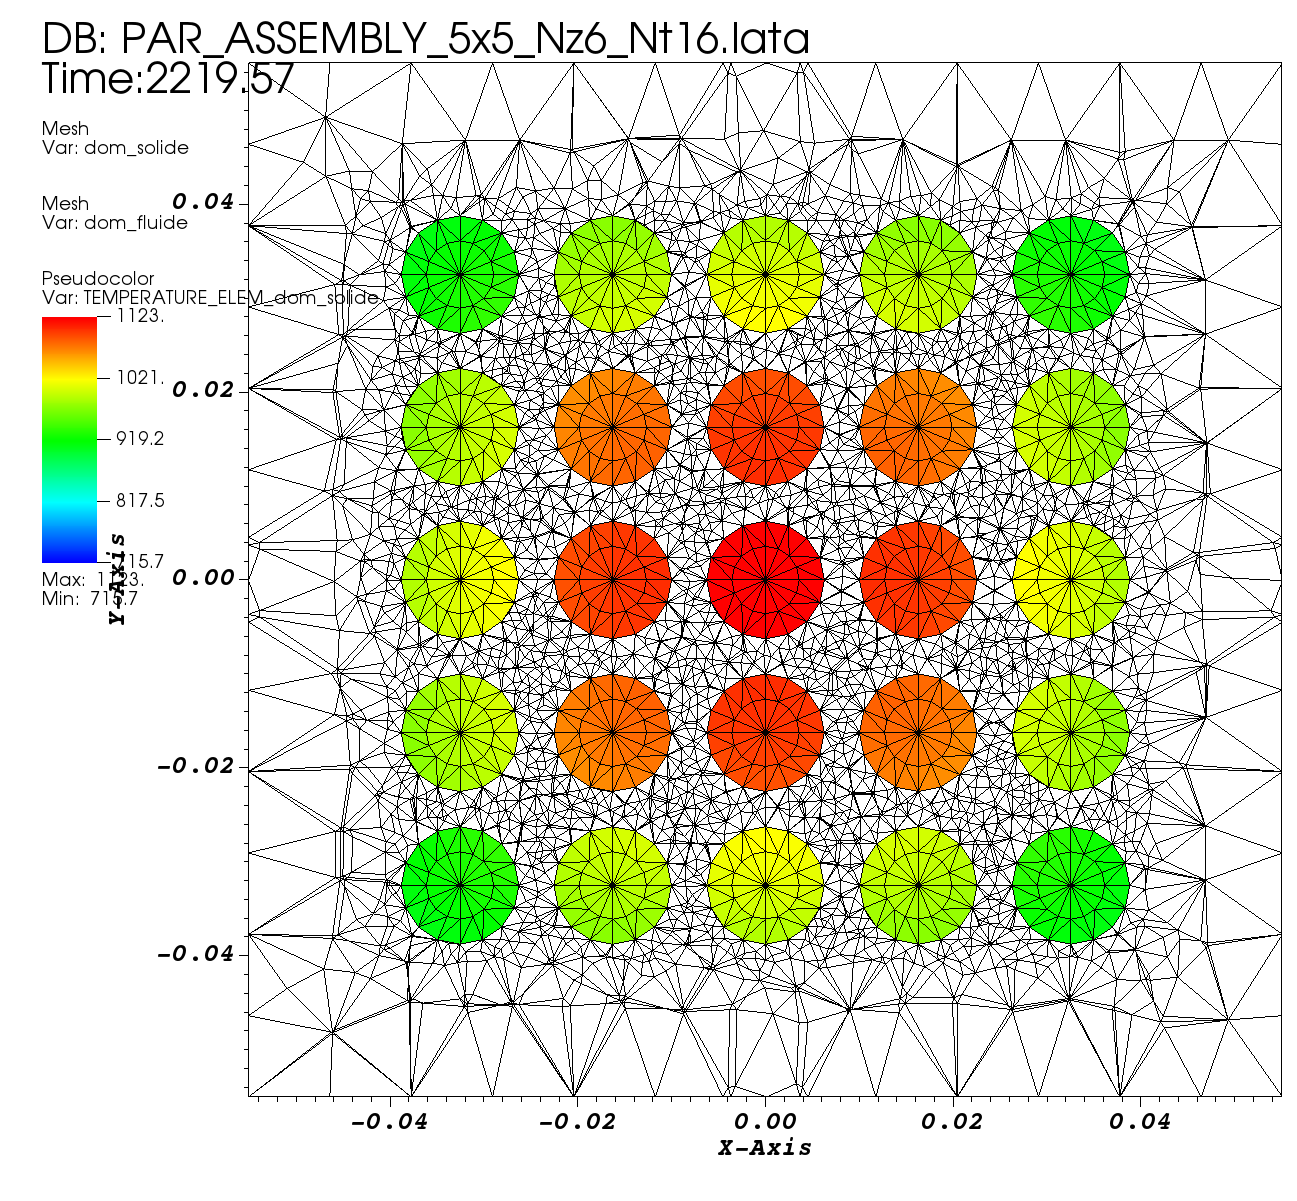
\includegraphics[width=\linewidth]{PICTURES/c5couplage/mesh_horizontal.png}
\end{minipage}
\hfill
\begin{minipage}{0.45\textwidth}
    \centering
    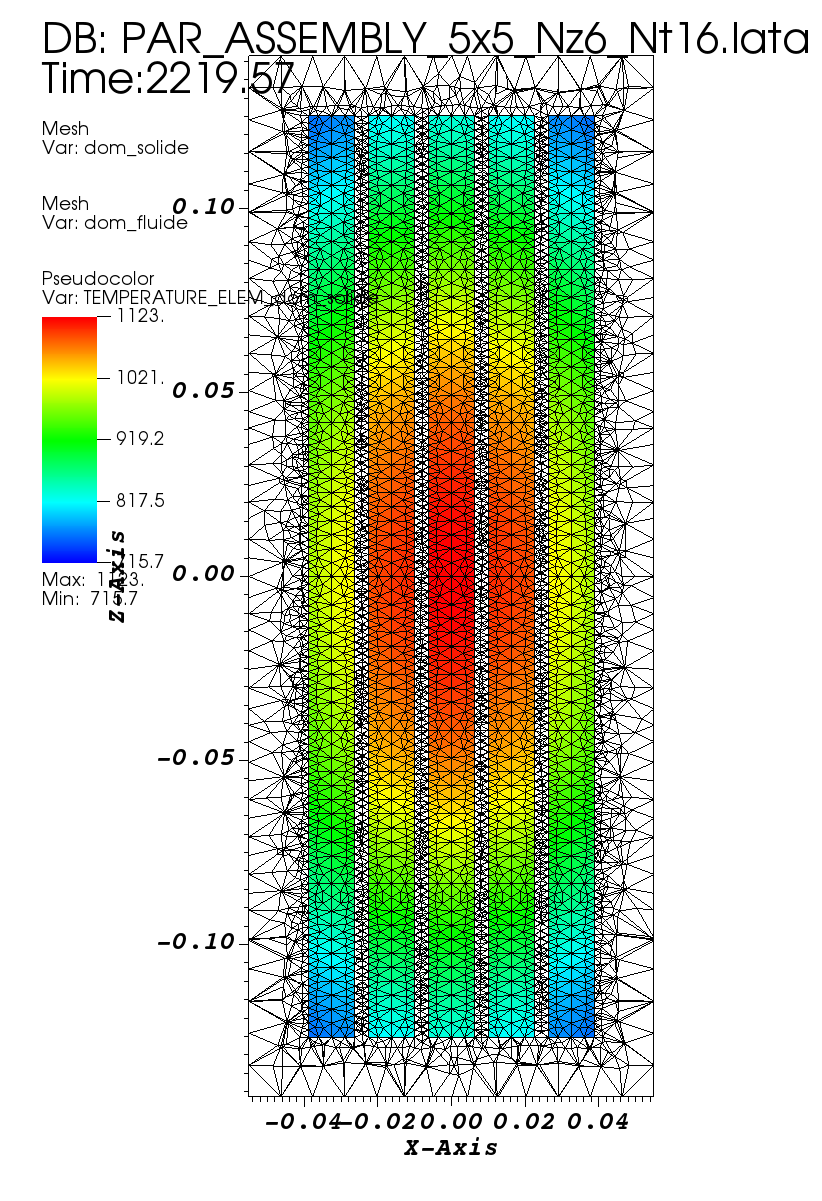
\includegraphics[width=\linewidth]{PICTURES/c5couplage/mesh_vertical.png}
\end{minipage}
\caption{Coupe horizontale en $Z=0$ (gauche) et coupe verticale (droite) du maillage volumique.}
\label{fig:mesh}
\end{figure}

\subsection{Discrétisation des faces radiatives}

Cette étude se concentre sur l'effet du raffinement axial de la discrétisation radiative, la sensibilité à la discrétisation radiale ayant déjà été étudiée en 2D par \cite{romain25}. La surface de chaque crayon est ainsi découpée, pour les besoins du calcul radiatif, en $N_\theta \times N_z$ sous-surfaces élémentaires, chacune résultant du croisement d'un secteur angulaire, hérité des $N_\theta = 16$ faces planes du maillage géométrique, avec une tranche axiale parmi les $N_z$ retenues. Le nombre de secteurs angulaires $N_\theta = 16$, fixé par des limitations des outils \salome et \trust, reste ainsi constant pour l'ensemble de cette étude. Seul le nombre de tranches axiales $N_z$ — paramètre propre à la discrétisation radiative, indépendant du maillage volumique — est varié, sur la plage $2, 4, \dots, 20$, afin de quantifier le biais introduit par l'hypothèse de radiosité uniforme au sein de chaque sous-surface.


\subsection{Stratégie de résolution numérique}

Le problème thermohydraulique couplé est résolu dans \textsc{Trust} par une méthode de volumes finis. Bien que l'objectif de cette étude soit d'obtenir l'état stationnaire du système, \textsc{Trust} résout ce problème par une approche de marche en temps : le schéma numérique fait converger la solution vers un point fixe stationnaire par intégration temporelle successive.

Le schéma retenu est un schéma d'Euler implicite, dont le pas de temps $\mathrm{d}t$ est piloté automatiquement entre les bornes $\mathrm{d}t_{\mathrm{min}}$ et $\mathrm{d}t_{\mathrm{max}}$ par un facteur de sécurité \texttt{facsec}. Ce facteur ajuste le pas de temps à chaque itération en fonction de la vitesse de convergence du solveur implicite, permettant d'accélérer la marche en temps tant que la convergence du système linéaire reste satisfaisante. Les principaux paramètres du schéma sont résumés en Annexe~ref{tab:solveur}.

La valeur de \texttt{facsec} retenue, très supérieure à l'unité, illustre bien la nature de cette stratégie : le pas de temps n'est plus piloté par un critère de précision physique de la dynamique transitoire, mais uniquement par la vitesse à laquelle le solveur implicite parvient à converger à chaque itération. Cette approche revient ainsi à utiliser l'intégration temporelle comme un simple outil numérique permettant d'atteindre efficacement l'état stationnaire recherché, sans chercher à représenter fidèlement une éventuelle dynamique transitoire réelle du système. Le calcul est considéré comme convergé lorsque l'évolution de la solution entre deux pas de temps successifs devient inférieure au seuil de stationnarité \texttt{seuil\_statio}.


\section{Résultats}

\subsection{Vérifications préliminaires}

Avant d'exploiter les résultats de température issus des simulations, deux vérifications préliminaires ont été menées afin de s'assurer de la cohérence physique du montage numérique.

La première concerne le profil de puissance imposé dans le combustible. La puissance volumique déposée devant suivre un profil axial en cosinus, représentatif de la distribution de puissance neutronique le long d'un crayon, le profil de température obtenu au centre du crayon central (Figure~\ref{fig:profil}) est comparé à ce profil attendu et montre une bonne adéquation avec les résultats de la simulation.

\begin{figure}[H]
\centering
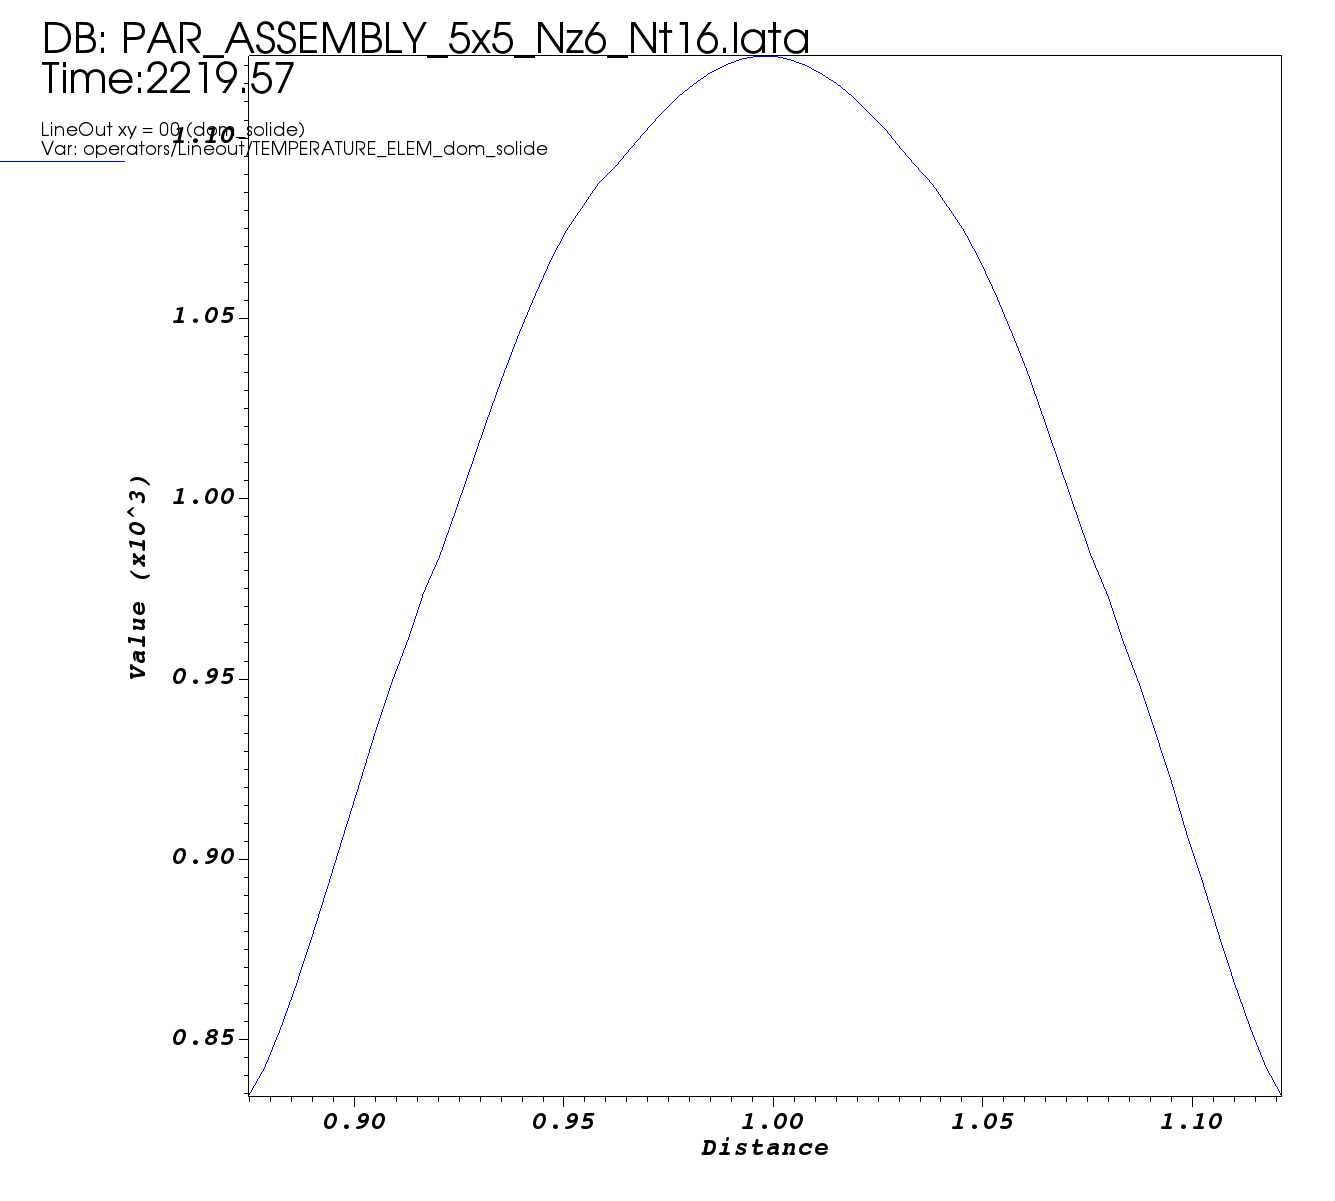
\includegraphics[width=0.4\linewidth]{PICTURES/c5couplage/lineout.png}
\caption{Profil axial de température au centre du crayon central.}
\label{fig:profil}
\end{figure}

La seconde vérification porte sur la conservation globale de l'énergie au sein du système. En régime stationnaire, la puissance totale déposée dans le combustible doit être intégralement évacuée par les mécanismes de transfert thermique du domaine, à savoir le rayonnement et la diffusion thermique à travers les parois du domaine. Le bilan global de puissance s'écrit ainsi :

\begin{equation}
    P_{\mathrm{déposée}} = P_{\mathrm{sortante}}, \qquad \text{avec } P_{\mathrm{sortante}} = P_{\mathrm{rad}} + P_{\mathrm{diffusion}},
    \label{eq:bilan_puissance}
\end{equation}

où $P_{\mathrm{déposée}}$ désigne la puissance volumique totale injectée dans le combustible, $P_{\mathrm{rad}}$ la puissance évacuée par rayonnement et $P_{\mathrm{diffusion}}$ celle évacuée par diffusion thermique à travers les parois du domaine. Cette égalité a été vérifiée sur l'ensemble des cas étudiés, avec un écart relatif compris entre quelques dizaines de pcm et $1\,\%$ selon les cas, confirmant, même dans la configuration la moins favorable, la cohérence du bilan thermique global de la simulation.


\subsection{Sensibilité à la discrétisation axiale}
\label{sec:consequence_radiosite}

La sensibilité de la solution thermique à la discrétisation axiale est étudiée pour trois niveaux de puissance représentatifs : $3$, $4$ et $45~\mathrm{MW/m^3}$, correspondant respectivement à des températures moyennes du crayon central d'environ $925$~K, $980$~K et $1817$~K. Le paramètre $N_z$ désigne le nombre de découpes selon l'axe $z$ des crayons; il ne s'agit pas d'un raffinement du maillage au sens numérique du terme, mais d'une discrétisation de la représentation des propriétés thermiques et radiatives, chaque sous-géométrie se voyant associer une température uniforme servant de température effective dans le calcul des échanges radiatifs.

Cette distinction est essentielle dans le cas étudié, où la puissance volumique suit un profil axial en cosinus, maximal au centre du domaine actif (Figure~\ref{fig:profil}). Une faible valeur de $N_z$ revient à homogénéiser thermiquement des portions axiales étendues du champ de température, tandis qu'une valeur élevée permet de résoudre les variations axiales locales. L'objectif de cette section est de quantifier l'influence de cette discrétisation sur les échanges radiatifs et sur le champ de température résultant.

Pour chaque niveau de puissance, les températures minimale, maximale et moyenne sont comparées à la solution de référence obtenue pour $N_z=20$, à partir de l'écart relatif

\begin{equation}
\varepsilon_T(N_z)
=
\frac{\left|T(N_z)-T(N_z=20)\right|}
{T(N_z=20)}.
\end{equation}

Avant d'analyser les résultats, il est utile de préciser l'origine physique de l'erreur introduite par cette représentation. Le flux surfacique net émis par rayonnement obéit, d'après l'Équation~\eqref{eq:nice_qr}, à \ref{def:radio}. Le caractère convexe de la fonction $T \mapsto T^4$ implique, d'après l'inégalité de Jensen, que pour toute distribution de température non uniforme discrétisée en $M$ éléments de surface égale au sein d'une sous-géométrie,

\begin{equation}
\overline{T^4}
=
\frac{1}{M}\sum_{k=1}^{M} T_k^4
\;>\;
\overline{T}^{\,4},
\qquad
\overline{T} = \frac{1}{M}\sum_{k=1}^{M} T_k,
\label{eq:jensen}
\end{equation}

l'égalité n'étant atteinte que pour un champ uniforme ($T_k$ identique $\forall k$).

\subsubsection{Cas $\overline{T} \approx 925{,}7~\mathrm{K}$}

La Figure~\ref{fig:temperature3MW} compare les champs de température obtenus avec $N_z=4$ et $N_z=20$, ainsi que leur différence. La Figure~\ref{fig:convergence3MW} présente l'évolution, en fonction de $N_z$, des écarts relatifs des températures minimale, maximale et moyenne par rapport à la solution de référence.

\begin{figure}[H]
\centering
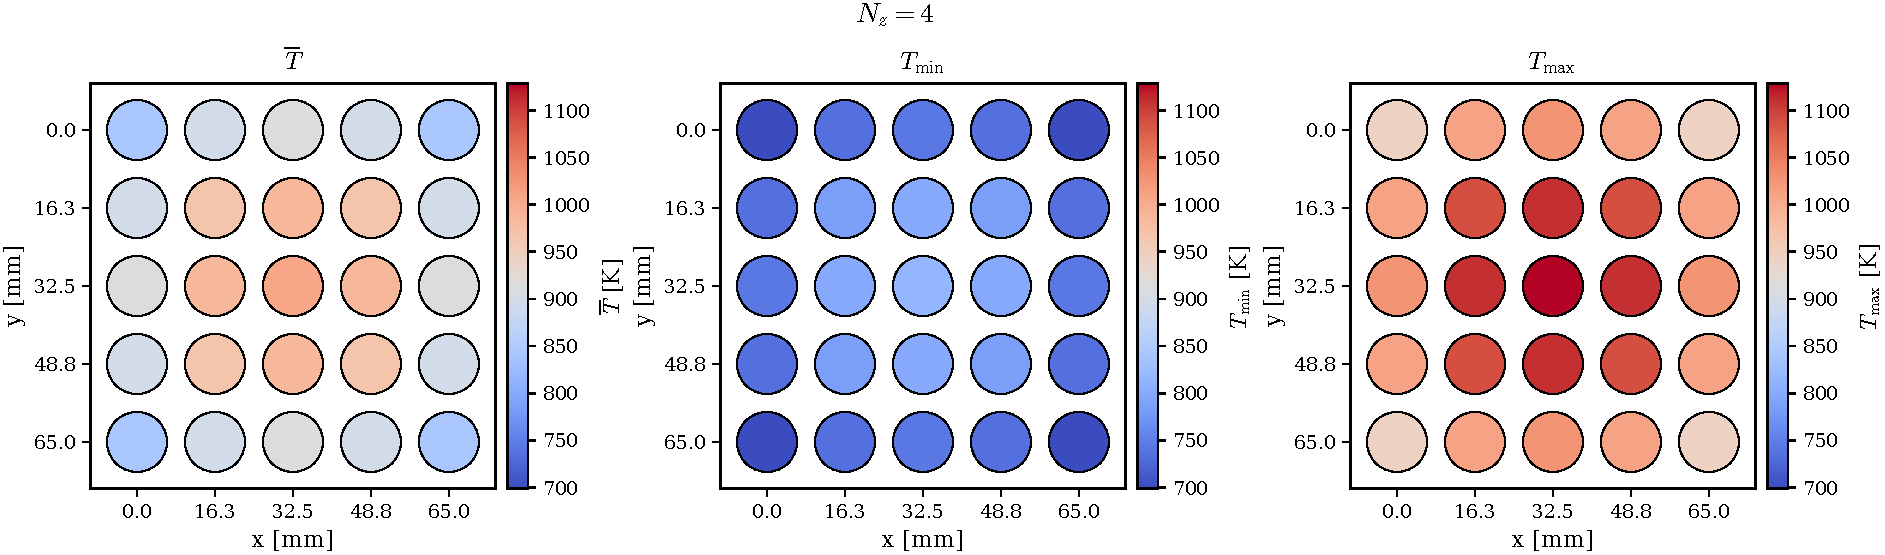
\includegraphics[width=0.8\linewidth]{PICTURES/c5couplage/T925/assembly_4.pdf}

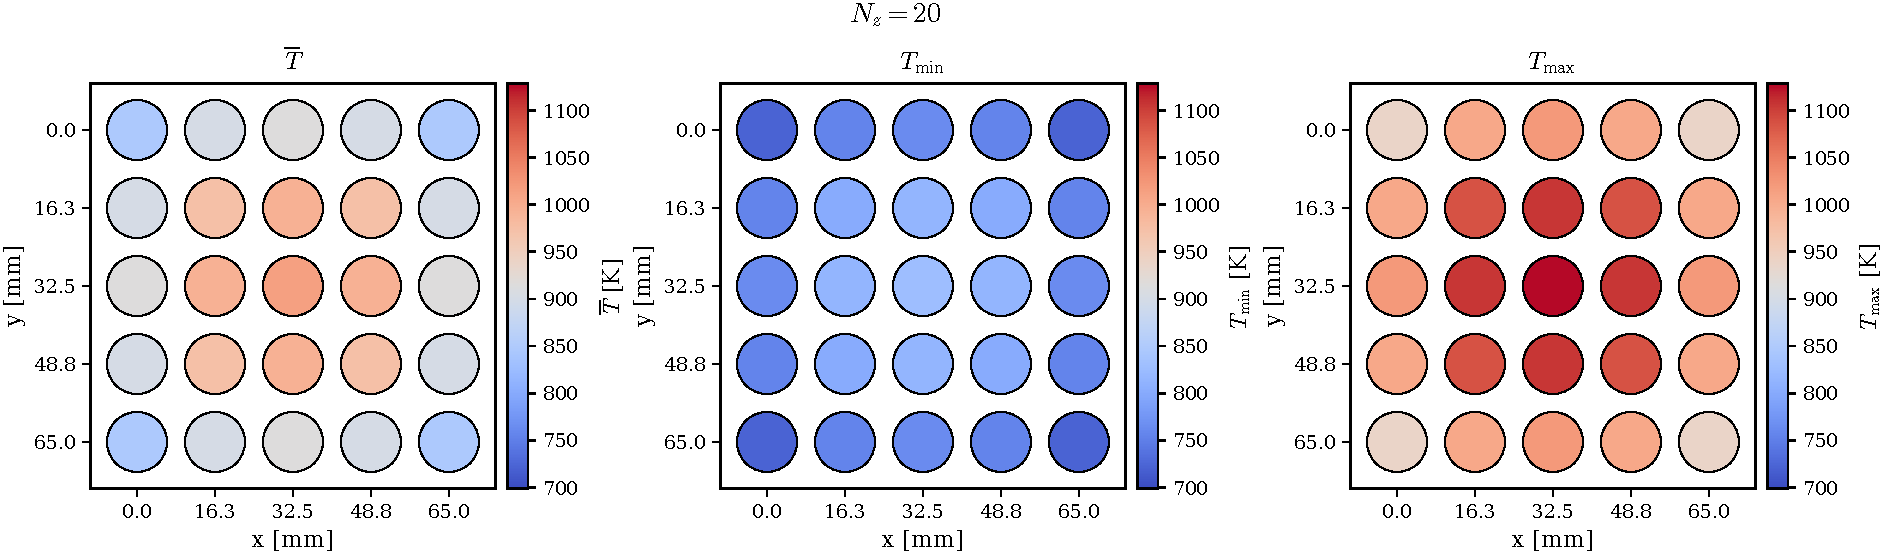
\includegraphics[width=0.8\linewidth]{PICTURES/c5couplage/T925/assembly_20.pdf}

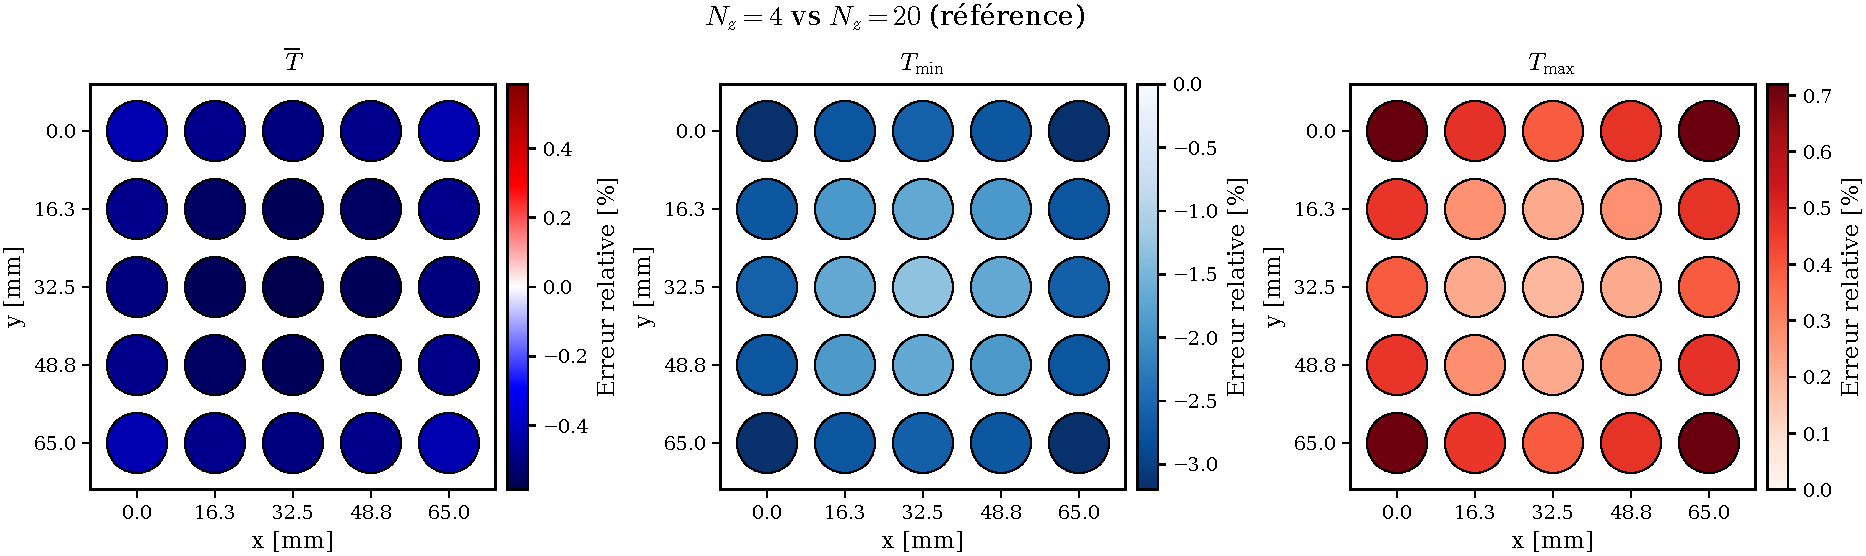
\includegraphics[width=0.8\linewidth]{PICTURES/c5couplage/T925/assembly_diff_4_vs_20.pdf}
\caption{Champs de température pour $\overline{T}=925{,}7~\mathrm{K}$ : $N_z=4$ (haut), $N_z=20$ (milieu) et différence entre les deux champs (bas).}
\label{fig:temperature3MW}
\end{figure}

\begin{figure}[H]
\centering
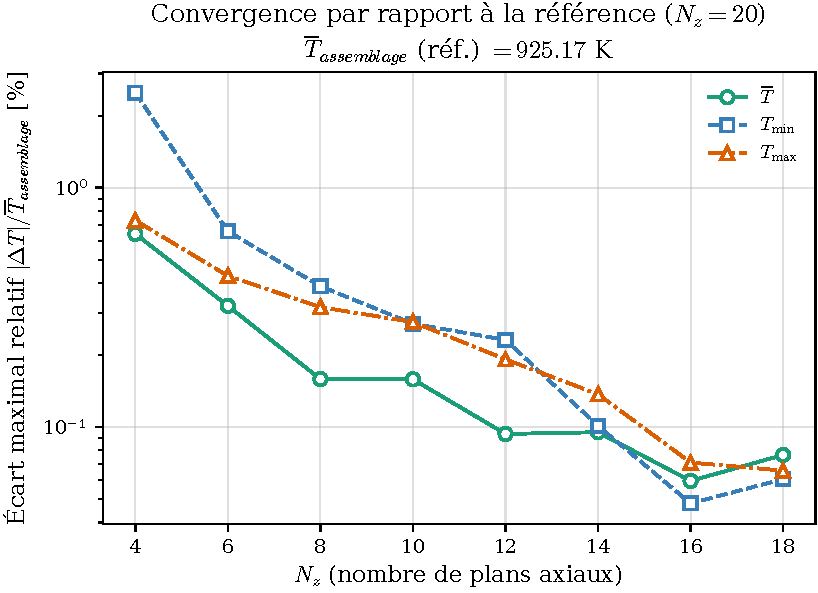
\includegraphics[width=0.7\linewidth]{PICTURES/c5couplage/T925/convergence_relative_vs_20.pdf}
\caption{Écart relatif des températures minimale, maximale et moyenne en fonction de $N_z$, par rapport à la référence $N_z=20$, pour $\overline{T}=925{,}7~\mathrm{K}$.}
\label{fig:convergence3MW}
\end{figure}

La Figure~\ref{fig:convergence3MW} met en évidence une convergence des trois grandeurs vers la solution de référence lorsque $N_z$ augmente : l'accroissement du raffinement axial permet de résoudre de plus en plus finement les variations thermiques axiales. Par exemple à partir de $N_z=14$, les écarts relatifs sont de l'ordre de $10^{-3}$, ce qui indique une bonne convergence du modèle.

Cette convergence s'interprète directement à la lumière de l'inégalité~\eqref{eq:jensen}. Dans chaque sous-géométrie, les propriétés radiatives sont évaluées à partir d'une température de surface uniforme. Une discrétisation axiale grossière assimile donc une portion étendue du profil thermique à une température unique, ce qui sous-estime la puissance rayonnée. Lorsque $N_z$ augmente, l'étendue axiale représentée par chaque température diminue, l'écart $\overline{T^4}-\overline{T}^{\,4}$ se réduit, et le bilan radiatif calculé tend vers celui du champ continu. Le raffinement axial ne constitue donc pas une simple amélioration: il détermine la fidélité avec laquelle le champ de température est \og vu \fg{} par le modèle radiatif.

La comparaison des champs de la Figure~\ref{fig:temperature3MW} montre par ailleurs que cette approximation ne modifie pas la structure thermique globale de l'assemblage : le crayon central demeure le plus chaud et les quatre crayons d'angle les plus froids, quelle que soit la valeur de $N_z$. Cette organisation spatiale est imposée par la géométrie de l'assemblage et par la configuration des échanges entre surfaces. La discrétisation axiale ne fait donc que moduler localement les niveaux de température, sans remettre en cause la hiérarchie thermique entre les crayons.

Les écarts sont en revanche nettement plus marqués sur les températures extrêmes que sur la température moyenne. Aux faibles valeurs de $N_z$, $T_{\max}$ est surestimée d'au plus $0{,}7\,\%$, tandis que $T_{\min}$ et $\overline{T}$ sont sous-estimées respectivement jusqu'à $3\,\%$ et $0{,}5\,\%$. Cette hiérarchie s'explique par la nature des grandeurs considérées : la température moyenne est une grandeur intégrée sur l'ensemble de l'assemblage, dans laquelle les erreurs locales de signes opposés se compensent partiellement, alors que $T_{\min}$ et $T_{\max}$ sont des grandeurs ponctuelles attachées aux régions les plus froides et les plus chaudes, précisément celles où les gradients --- et donc l'écart de l'inégalité~\eqref{eq:jensen} --- sont les plus importants.

Le signe de l'écart sur $T_{\max}$ s'interprète dans la région centrale, où le profil de puissance est maximal. Lorsque plusieurs positions axiales sont regroupées dans une même sous-géométrie, la température homogénéisée y est inférieure à la température réellement atteinte au point chaud. D'après l'inégalité~\eqref{eq:jensen}, la puissance radiative émise par cette sous-géométrie est alors sous-estimée : le puits radiatif est trop faible, et l'équilibre thermique local ne peut être rétabli qu'au prix d'une élévation de la température. Il en résulte une surestimation de $T_{\max}$ par rapport à la solution finement discrétisée.

Le comportement de $T_{\min}$ relève d'un mécanisme différent. La température des régions froides ne dépend pas seulement de leur propre émission : elle résulte du bilan entre la puissance radiative reçue des surfaces chaudes environnantes, leurs pertes radiatives et les transferts conductifs au sein de l'assemblage. La sous-estimation des émissions dans les zones chaudes voisines se propage donc, via le réseau des échanges radiatifs, jusqu'aux régions froides. L'écart observé sur $T_{\min}$ n'est ainsi pas la conséquence directe d'une moyenne locale, mais la signature du couplage entre la non-linéarité du rayonnement et la redistribution thermique à l'échelle de l'assemblage.

\begin{table}[H]
\centering
\caption{Écarts relatifs maximaux observés par rapport à la référence $N_z=20$ pour $\overline{T}=925{,}7~\mathrm{K}$.}
\label{tab:ecarts_discretisation_axiale}
\begin{tabular}{lcc}
\hline
Grandeur & Sens de l'écart & Écart maximal \\
\hline
$T_{\max}$ & Surestimation & $+0{,}7\,\%$ \\
$T_{\min}$ & Sous-estimation & $-3{,}0\,\%$ \\
$\overline{T}$ & Sous-estimation & $-0{,}5\,\%$ \\
\hline
\end{tabular}
\end{table}

Il convient enfin de s'assurer que ces écarts ne proviennent pas de la précision intrinsèque de la résolution numérique. Le critère de convergence du solveur thermique garantit une stabilisation de la température moyenne à environ $0{,}1~\mathrm{K}$, soit, pour $\overline{T}\approx925{,}7~\mathrm{K}$, une incertitude relative de
\begin{equation}
\frac{0{,}1}{925{,}7} \approx 1{,}1\times10^{-4}.
\end{equation}
Cette incertitude est inférieure d'au moins un ordre de grandeur aux écarts relatifs obtenus pour les discrétisations les plus grossières. Les différences observées entre les solutions sont donc bien attribuables à la discrétisation axiale et à son influence sur la représentation des échanges radiatifs, et non à une convergence insuffisante du solveur.

Pour ce niveau de puissance, un raffinement jusqu'à $N_z=14$ suffit ainsi à obtenir une représentation peu baisée la poursuite du raffinement devient peu pertinente, l'erreur de discrétisation étant déjà faible devant les autres sources d'incertitude du modèle : le choix de $N_z$ résulte d'un compromis entre la précision du bilan radiatif et le coût de calcul.


\subsubsection{Cas $\overline{T} \approx 981{,}4~\mathrm{K}$}

Comme pour le cas précédent, la solution converge vers l'état de référence $N_z=20$ sans modification de la structure thermique globale (crayon central le plus chaud, crayons d'angle les plus froids). Les résultats détaillés sont disponibles en Annexe~\ref{annexe:resultats}. L'amplitude des écarts augmente cependant légèrement avec le niveau de puissance, restant néanmoins concentrée sur les températures extrêmes (Tableau~\ref{tab:ecarts_discretisation_axiale_4MW}), conformément à la sensibilité en $T^4$ des échanges radiatifs. La convergence du solveur ($\sim 10^{-4}$ d'incertitude relative) reste très inférieure à ces écarts, confirmant qu'ils sont bien imputables à la discrétisation axiale.

\begin{table}[H]
\centering
\caption{Écarts relatifs maximaux observés par rapport à la référence $N_z=20$ pour $\overline{T}=981{,}4~\mathrm{K}$.}
\label{tab:ecarts_discretisation_axiale_4MW}
\begin{tabular}{lcc}
\hline
Grandeur & Sens de l'écart & Écart maximal \\
\hline
$T_{\max}$ & Surestimation & $+0{,}9\,\%$ \\
$T_{\min}$ & Sous-estimation & $-4{,}0\,\%$ \\
$\overline{T}$ & Sous-estimation & $-0{,}5\,\%$ \\
\hline
\end{tabular}
\end{table}

\subsubsection{Cas $\overline{T} \approx 1817~\mathrm{K}$}

La Figure~\ref{fig:temperature45MW} compare les champs de température obtenus avec $N_z=4$ et $N_z=20$, ainsi que leur différence. La Figure~\ref{fig:convergence45MW} présente l'évolution des écarts relatifs en fonction de $N_z$, par rapport à la solution de référence.

\begin{figure}[H]
\centering
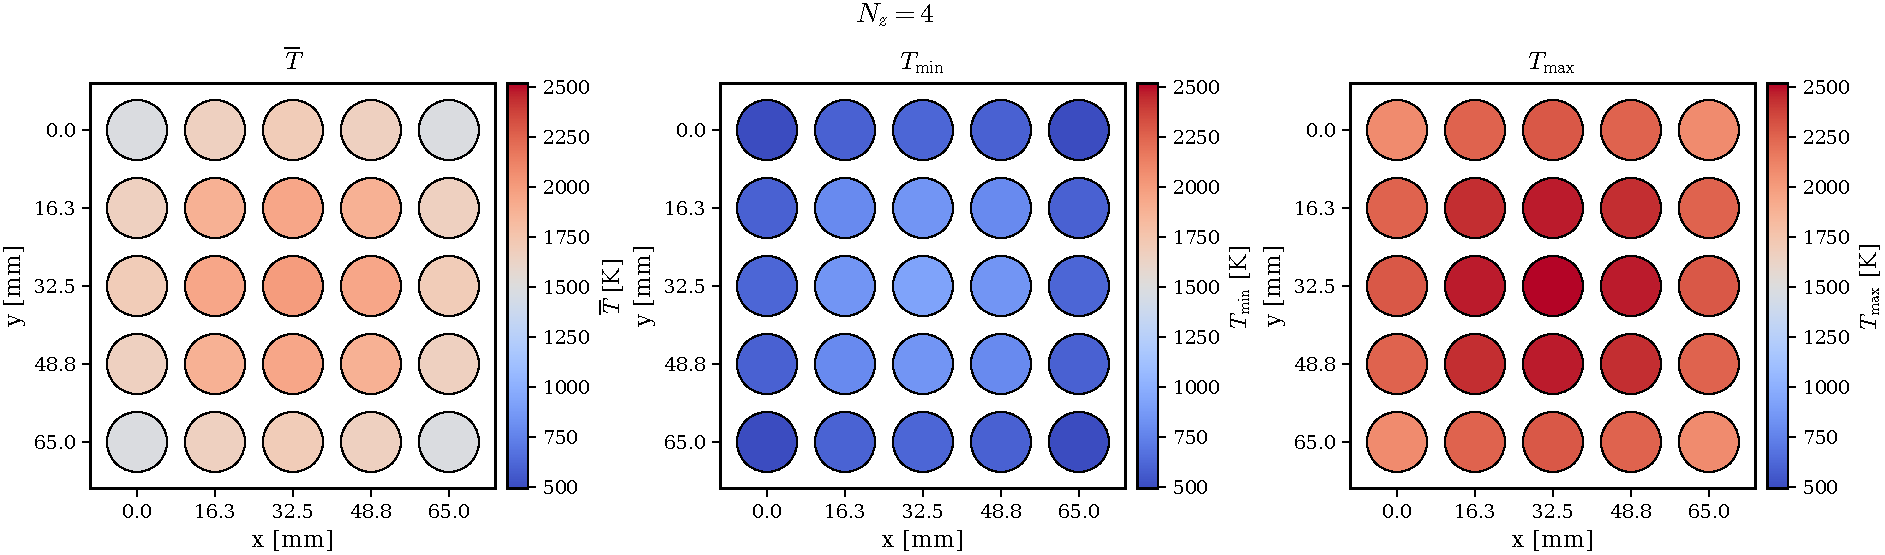
\includegraphics[width=0.8\linewidth]{PICTURES/c5couplage/T1800/assembly_4.pdf}

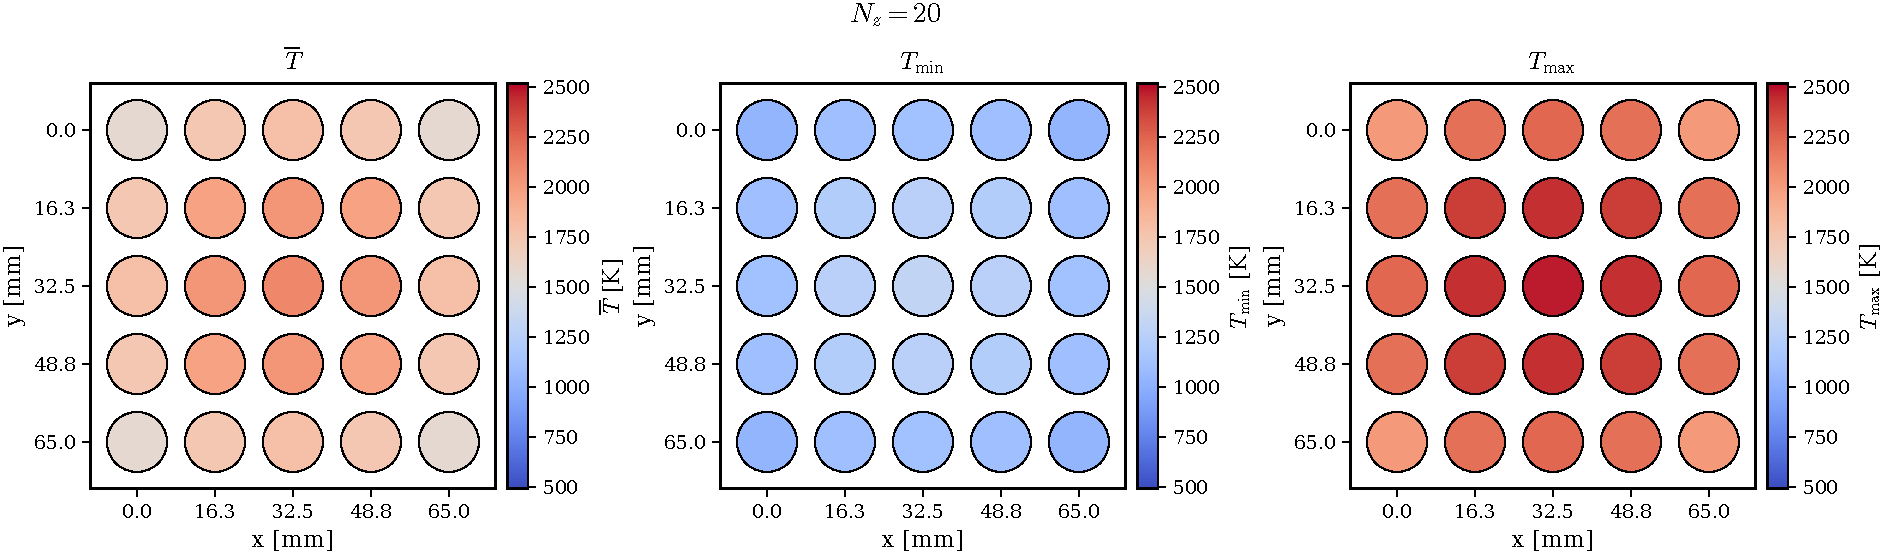
\includegraphics[width=0.8\linewidth]{PICTURES/c5couplage/T1800/assembly_20.pdf}

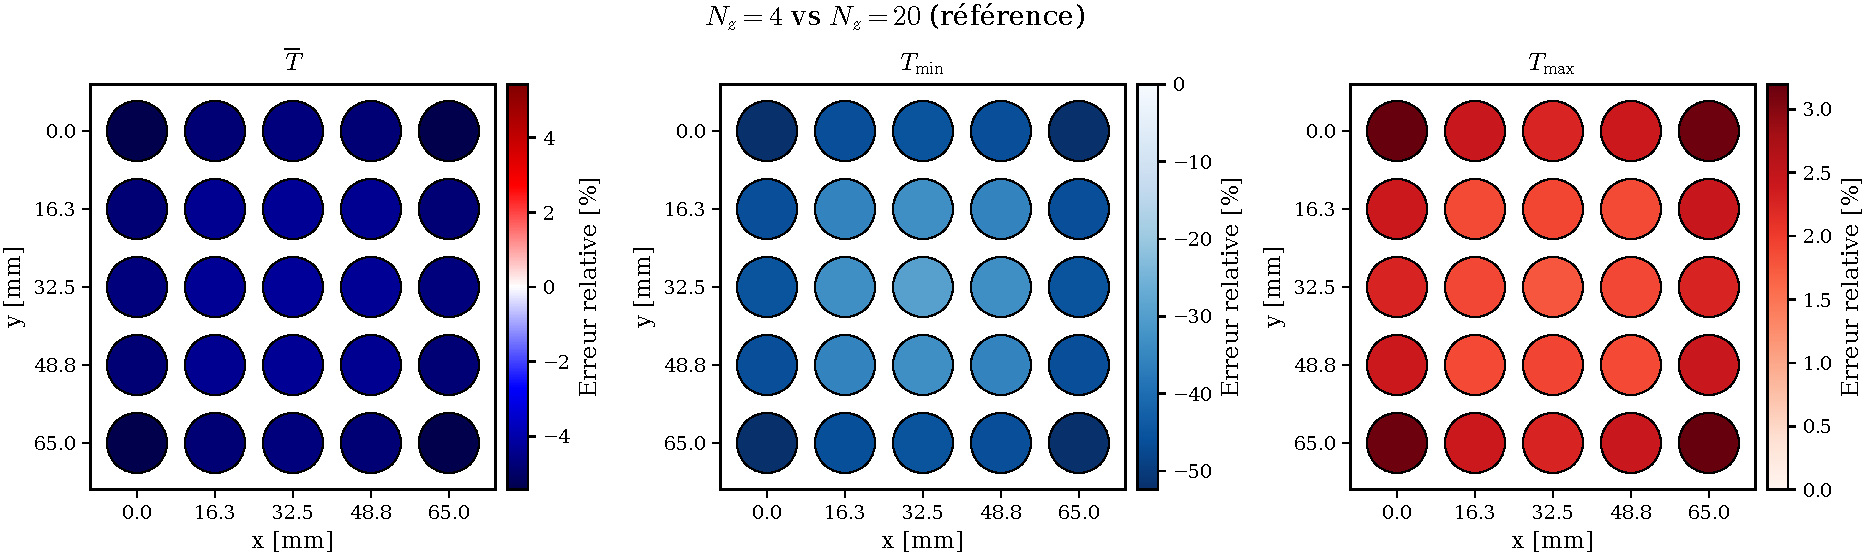
\includegraphics[width=0.8\linewidth]{PICTURES/c5couplage/T1800/assembly_diff_4_vs_20.pdf}
\caption{Champs de température pour le niveau de puissance le plus élevé : $N_z=4$ (haut), $N_z=20$ (milieu) et différence entre les deux champs (bas).}
\label{fig:temperature45MW}
\end{figure}

\begin{figure}[H]
\centering
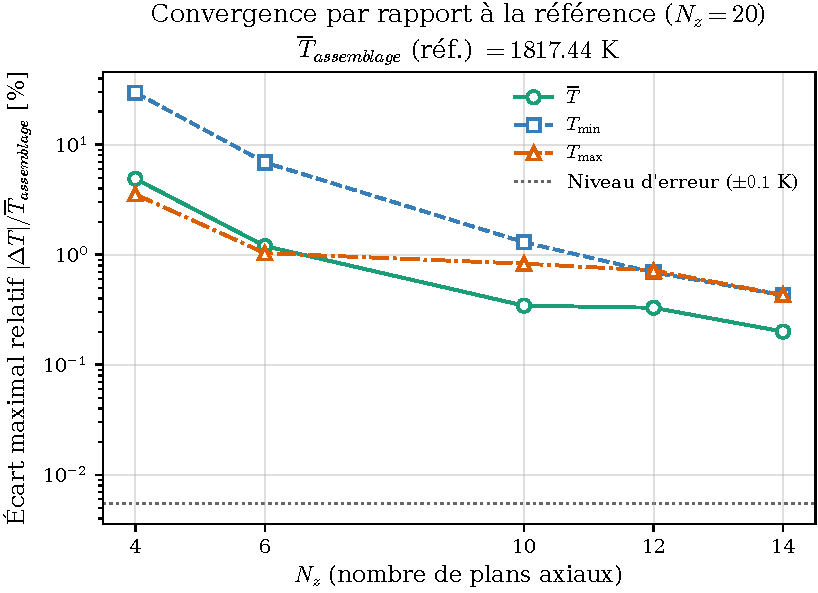
\includegraphics[width=0.7\linewidth]{PICTURES/c5couplage/T1800/convergence_relative_vs_20.pdf}
\caption{Écart relatif des températures minimale, maximale et moyenne en fonction de $N_z$, par rapport à la référence $N_z=20$, pour le niveau de puissance le plus élevé.}
\label{fig:convergence45MW}
\end{figure}

La Figure~\ref{fig:convergence45MW} montre que l'influence de la discrétisation axiale change qualitativement de régime pour ce niveau de puissance. La convergence vers la solution de référence est toujours observée, mais les écarts aux faibles valeurs de $N_z$ atteignent désormais des amplitudes d'un autre ordre : $T_{\max}$ est surestimée jusqu'à $3\,\%$, tandis que $T_{\min}$ et $\overline{T}$ sont sous-estimées respectivement jusqu'à $52\,\%$ et $5\,\%$.

\begin{table}[H]
\centering
\caption{Écarts relatifs maximaux observés par rapport à la référence $N_z=20$ pour $\overline{T}=1817~\mathrm{K}$.}
\label{tab:ecarts_discretisation_axiale_dernier}
\begin{tabular}{lcc}
\hline
Grandeur & Sens de l'écart & Écart maximal \\
\hline
$T_{\max}$ & Surestimation & $+3\,\%$ \\
$T_{\min}$ & Sous-estimation & $-52\,\%$ \\
$\overline{T}$ & Sous-estimation & $-5\,\%$ \\
\hline
\end{tabular}
\end{table}

Ces résultats constituent une rupture nette par rapport aux deux niveaux de puissance précédents : alors que la température moyenne n'était affectée que de $0{,}5\,\%$ au plus, son écart atteint ici $5\,\%$, et celui sur $T_{\min}$ dépasse $50\,\%$. La discrétisation grossière ne produit donc pas une erreur uniforme sur le champ thermique : elle affecte de manière disproportionnée les régions froides et les grandeurs qui leur sont attachées.

Ce changement de régime résulte de l'augmentation simultanée du niveau de température et des gradients thermiques. À cette puissance, les écarts de température entre régions de l'assemblage deviennent considérables ; une sous-géométrie couvrant une portion axiale étendue regroupe alors des zones dont les températures diffèrent fortement, et l'écart $\overline{T^4}-\overline{T}^{\,4}$ de l'inégalité~\eqref{eq:jensen} croît d'autant. La température homogénéisée cesse d'être représentative des conditions locales, et l'erreur commise sur le bilan radiatif devient suffisamment importante pour modifier le champ thermique lui-même.

Cette propagation explique également que la température moyenne soit désormais affectée de manière non négligeable. Un écart de $5\,\%$ ne peut plus relever d'une perturbation locale s'annulant par compensation spatiale : il traduit une modification du bilan radiatif suffisamment significative pour déplacer l'équilibre thermique global de l'assemblage.

La température maximale reste comme pour les autres cas moins sensible, son écart ne passant que de $0{,}9\,\%$ à $3\,\%$.

Comme pour les cas précédents, la convergence du solveur ne saurait expliquer ces écarts : avec une température moyenne stabilisée à $0{,}1~\mathrm{K}$ près, l'incertitude relative associée est de l'ordre de
\begin{equation}
\frac{0{,}1}{1817}
\approx 5{,}5\times10^{-5},
\end{equation}
soit près de trois ordres de grandeur en dessous des écarts mesurés. Ceux-ci sont donc bien attribuables à la représentation axiale des échanges radiatifs.

Ce dernier cas met ainsi en évidence une limite intrinsèque du modèle de discrétisation axiale. Alors que des valeurs modérées de $N_z$ suffisent aux deux premiers niveaux de puissance, elles deviennent inacceptables lorsque le niveau de température et les gradients thermiques augmentent fortement : une erreur de $52\,\%$ sur $T_{\min}$ et de $5\,\%$ sur la température moyenne signifie qu'une discrétisation trop grossière ne fausse plus seulement les valeurs locales, mais le bilan thermique global de l'assemblage. Le choix de $N_z$ ne peut donc pas être fixé sur la seule base d'un cas à puissance modérée ; il doit être établi en tenant compte du niveau de température et de l'intensité des gradients attendus sur l'ensemble des configurations étudiées.

Cette analyse confirme que le raffinement axial est un paramètre déterminant pour la représentativité du calcul radiatif. Aux niveaux de puissance les plus élevés, une discrétisation suffisamment fine est indispensable pour limiter l'erreur associée à l'hypothèse de radiosité unfirome et température constance par surface et garantir une précision acceptable sur l'ensemble du champ thermique, en particulier dans les régions les plus froides.

\subsection{Étude de l'écart entre le point chaud et la température moyenne}

Le Tableau~\ref{tab:tmoy_tmax} rassemble, pour les différents niveaux de puissance étudiés, la température moyenne de l'assemblage $T_{\mathrm{moy}}$ et la température de point chaud du système. Pour des raisons de compromis entre temps de calcul et convergence, une découpe en 14 sections axiales a été choisie. Le biais lié à l'hypothèse de radiosité uniforme est alors de l'ordre du pour mille. Cette étude correspond au maximum des températures maximales relevées sur l'ensemble des crayons de l'assemblage, $T_{\mathrm{max}} = \max_i \left( T_{\mathrm{max},i} \right)$, qui coïncide avec la température maximale du crayon central, celui-ci étant le plus exposé thermiquement du fait de sa position au cœur de l'assemblage. On observe que l'écart entre $T_{\mathrm{max}}$ et $T_{\mathrm{moy}}$ croît avec le niveau de puissance déposée, aussi bien en valeur absolue qu'en proportion de la température moyenne.

L'intérêt de ce résultat ne réside pas uniquement dans ces valeurs prises isolément, mais dans la démarche qu'elles illustrent : la capacité à quantifier, à partir d'une simulation CFD 3D convergée, l'écart entre température moyenne et température de point chaud pour une configuration donnée. Une telle relation, une fois établie sur un nombre suffisant de cas, ouvrirait la voie à l'estimation de la température de point chaud d'un système à partir de sa seule température moyenne, cette dernière étant directement accessible par des modèles à zones plus simples et bien moins coûteux en temps de calcul que la simulation CFD 3D complète.

Il convient toutefois de discuter dans quelle mesure ce résultat dépend du profil de puissance retenu. Le profil axial en cosinus utilisé dans cette étude, représentatif de la distribution de puissance neutronique le long d'un crayon, concentre le dépôt de puissance au centre du domaine actif et atténue les effets de bord en haut et en bas du crayon. Ce choix exacerbe mécaniquement l'écart $T_{\mathrm{max}} - T_{\mathrm{moy}}$ par rapport à un profil plat, mais il correspond à des situations physiquement réalistes en réacteur. La position du point chaud (crayon central, cote axiale médiane) ne varie pas avec le niveau de puissance étudié, ce qui conforte la robustesse de la corrélation établie.

La modélisation de l'écart relatif en fonction de la température moyenne, présentée en Figure~\ref{fig:hotspot}, s'ajuste par une loi de la forme
\begin{equation}
\frac{T_{\mathrm{max}} - T_{\mathrm{moy}}}{T_{\mathrm{moy}}} = A + C \exp\left(-\frac{T_{\mathrm{moy}}}{\tau}\right),
\end{equation}
avec $A$, $C$ et $\tau$ des paramètres ajustés sur les données. Cette expression traduit la saturation progressive de l'écart relatif aux températures élevées, où le transfert radiatif tend à homogénéiser le champ thermique. La faisabilité d'une telle démarche sur un assemblage $5\times5$, bien que simplifié par rapport à une géométrie de cœur réel, démontre le potentiel de cette approche pour des configurations industrielles plus représentatives.

\begin{table}[H]
\centering
\begin{tabular}{cccc}
\toprule
Puissance volumique~[$\mathrm{MW/m^3}$] & $T_{\mathrm{moy}}$~[K] & $T_{\mathrm{max}}$~[K] & Écart relatif $\frac{T_{\mathrm{max}} - T_{\mathrm{moy}}}{T_{\mathrm{moy}}}$ \\
\midrule
$3$  & $925{,}2$ & $1127$ & $21{,}81\,\%$ \\
$4$  & $981{,}5$ & $1211$ & $23{,}38\,\%$ \\
$5$  & $1028$    & $1280$ & $24{,}51\,\%$ \\
$10$ & $1215$    & $1560$ & $28{,}40\,\%$ \\
$20$ & $1453$    & $1915$ & $31{,}80\,\%$ \\
$30$ & $1621$    & $2170$ & $33{,}87\,\%$ \\
$40$ & $1756$    & $2376$ & $35{,}31\,\%$ \\
$45$ & $1817$    & $2475$ & $36{,}21\,\%$ \\
\bottomrule
\end{tabular}
\caption{Température moyenne de l'assemblage et température de point chaud (crayon central) pour les niveaux de puissance étudiés.}
\label{tab:tmoy_tmax}
\end{table}

\begin{figure}[H]
\centering
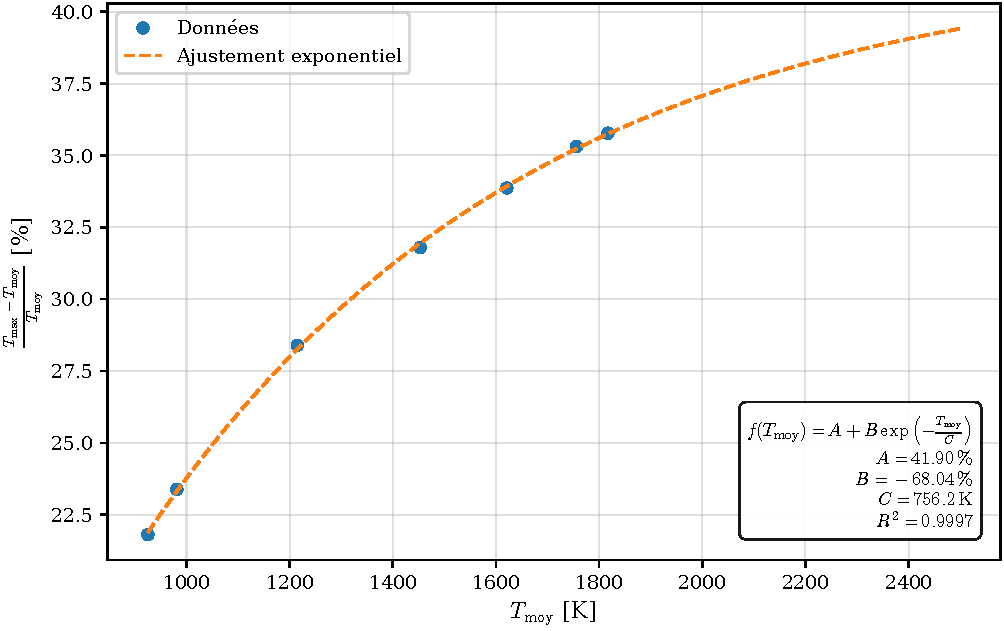
\includegraphics[width=0.7\linewidth]{PICTURES/c5couplage/hot_spot.pdf}
\caption{Modélisation de l'écart de la température maximale par rapport à la température moyenne.}
\label{fig:hotspot}
\end{figure}


\subsection{Conclusion}

Ce chapitre a permis de démontrer la faisabilité d'une étude CFD 3D couplée conduction--rayonnement sur une géométrie représentative d'un assemblage de crayons combustible en réseau $5\times5$. À travers une campagne de simulations paramétriques, trois résultats principaux ont été mis en évidence.

\textbf{Premièrement}, la discrétisation axiale des surfaces dans le calcul radiatif constitue un paramètre déterminant pour la précision du bilan thermique global. L'inégalité de Jensen, appliquée à la loi de Stefan--Boltzmann, fournit le cadre théorique permettant de comprendre pourquoi l'homogénéisation de la température par sous-géométrie sous-estime systématiquement la puissance radiative émise dès qu'un gradient thermique est présent. Cette sous-estimation se propage à travers le réseau d'échanges radiatifs et affecte de manière significative les températures du système et mérite d'être étudié en profondeur.

\textbf{Deuxièmement}, l'amplitude de l'erreur induite par une discrétisation grossière croît fortement avec le niveau de puissance déposée. Aux faibles puissances ($3$ et $4~\mathrm{MW/m^3}$), un nombre de tranches axiales $N_z = 14$ suffit à garantir des écarts relatifs inférieurs au pour cent sur la température moyenne et aux températures extrêmes. En revanche, à forte puissance ($45~\mathrm{MW/m^3}$), une discrétisation identique conduit à des écarts de $52\,\%$ sur $T_{\min}$ et de $5\,\%$ sur $\overline{T}$, traduisant une modification du bilan thermique global de l'assemblage. Le choix de $N_z$ ne peut donc pas être fixé une fois pour toutes : il doit être adapté au régime thermique considéré.

\textbf{Troisièmement}, la simulation CFD 3D offre la possibilité d'établir une corrélation entre température moyenne et température de point chaud. L'écart relatif $T_{\mathrm{max}} - T_{\mathrm{moy}}$ croît avec la puissance déposée et peut être modélisé par une loi de saturation, ouvrant la voie à une estimation de la température de point chaud à partir de modèles à zones plus simples et moins coûteux. La position du point chaud (crayon central, cote axiale médiane) se révèle invariante avec le niveau de puissance, ce qui renforce la robustesse de cette approche.

Ces travaux ouvrent plusieurs perspectives. L'extension de cette démarche à des géométries industrielles plus représentatives, incluant notamment des assemblages de plus grande taille et des profils de puissance plus complexes, permettrait de valider la généralité de la corrélation établie. Par ailleurs, l'étude de l'influence conjointe des discrétisations angulaire et axiale sur la précision du calcul radiatif constituerait un prolongement naturel de cette analyse. Enfin, l'intégration de cette corrélation dans un modèle à zones amélioré permettrait de combiner la rapidité de calcul des approches simplifiées avec la précision des simulations CFD 3D sur les grandeurs critiques de sûreté.

	

	

\chapter*{Conclusion}
\addcontentsline{toc}{chapter}{Conclusion}

Le rayonnement thermique constitue un mécanisme de transfert de chaleur incontournable dès lors que les températures deviennent élevées, que ce soit en régime nominal dans les réacteurs à haute température de type HTGR, ou en situation accidentelle dans les réacteurs à eau légère. La simulation de ces échanges radiatifs, en particulier dans des géométries tridimensionnelles complexes, constitue ainsi un enjeu important pour la plateforme multiphysique \trust du CEA.

Ce stage s'est inscrit dans cette problématique, avec pour objectif de consolider, d'étendre et de vérifier un module de calcul radiatif par lancer de rayons Monte Carlo (\emb), développé à partir d'une première maquette héritée d'un précédent stage. Ce travail a couvert l'ensemble de la chaîne de développement d'un tel outil : l'écriture du module en C++, avec une attention particulière portée aux problématiques de calcul haute performance (parallélisation, vectorisation), la mise en place d'une démarche de vérification rigoureuse du code au moyen de solutions analytiques et de comparaisons à un code de référence, puis la mise en œuvre de l'ensemble de la chaîne de simulation sur un cas d'étude représentatif, un assemblage de crayons combustible couplant calcul radiatif et simulation thermohydraulique 3D au sein de TRUST.

Cette dernière étape a nécessité la mise en commun de l'ensemble des briques développées au cours du stage : la prise en main de la plateforme \salome pour la génération des maillages surfaciques et volumiques, l'utilisation de TRUST pour la résolution du problème thermohydraulique couplé, ainsi que le développement de nombreux utilitaires Python dédiés au post-traitement des résultats, à la génération automatisée des maillages et à la création des fichiers d'entrée TRUST. Cette diversité d'outils, a ainsi pu être mobilisée de façon cohérente pour aboutir aux résultats du cas d'étude final.

Sur le plan personnel, ce stage a été l'occasion d'un apprentissage significatif du langage C++, jusqu'alors peu maîtrisé, appliqué directement à un contexte de calcul scientifique exigeant en performance. Il a également permis d'approfondir mes connaissances en transfert radiatif, en particulier dans le cas des milieux transparents entre surfaces opaques, ainsi que ma compréhension des enjeux propres à la vérification et à la validation d'un code de simulation. Enfin, la prise en main de deux outils centraux de l'écosystème logiciel du CEA, \trust et \salome, constitue un acquis qui dépasse le seul cadre de ce stage.

Ce travail ouvre plusieurs perspectives. Sur le plan fonctionnel, il ouvre la voie au développement de modèles à zones en trois dimensions, capables de tirer parti du module radiatif développé pour dépasser les limites des approches actuelles. Une telle démarche nécessiterait cependant d'explorer des méthodes alternatives au modèle des facteurs de vue d'ordre 1 utilisé dans ce rapport, afin de s'affranchir de l'hypothèse de radiosité uniforme dont l'étude du chapitre précédent a montré les limites. Plus largement, ce stage aura permis de partir d'une preuve de concept portant sur un modèle de rayonnement 3D pour aboutir à une preuve de concept de calcul CFD couplé, mettant en évidence la viabilité de cette chaîne de simulation pour des cas d'usage représentatifs. Enfin, ce travail mené en milieu transparent constitue également un premier pas vers ma thèse, intitulée \textit{Transferts de chaleur par rayonnement : résolution numérique efficace de problèmes associés en milieu beerien ou non pour les besoins de validation de modèles simplifiés}, qui prolongera cette démarche à des milieux participants.
	
		\renewcommand{\thechapter}{}
	\renewcommand{\thesection}{\Alph{section}}
	\setcounter{section}{0}	

	\chapter{Annexes}
%\section{Annexe}
\subsection{Résolution intégrale des facteurs de vue}
\label{method_integrale}
On considère le facteur de vue entre deux faces opposées d'un cube unité : la face $z=0$ (surface $A_1$) et la face $z=1$ (surface $A_2$). Le facteur de vue est défini de manière générale par :
\begin{equation}
F_{16}=\frac{1}{A_1}\int_{A_1}\int_{A_2}\frac{\cos\theta_1 \cos\theta_2}{\pi R^2}\, dA_2\, dA_1.
\end{equation}

Dans le cas du cube unité, on a $A_1=A_2=1$. Les deux faces étant parallèles, on paramètre les surfaces par :
\begin{align}
P_1=(x,y,0), \quad (x,y)\in[0,1]^2,\\
P_2=(x',y',1), \quad (x',y')\in[0,1]^2.
\end{align}

La distance entre deux éléments différentiels s'écrit :
\begin{equation}
R^2=(x'-x)^2+(y'-y)^2+1.
\end{equation}

\paragraph{Calcul des cosinus directionnels}

Les normales aux surfaces sont :
\begin{equation}
\mathbf n_1=(0,0,1), \qquad \mathbf n_2=(0,0,-1).
\end{equation}

Le vecteur reliant les deux points est :
\begin{equation}
\mathbf r=(x'-x,\;y'-y,\;1), \qquad R=\|\mathbf r\|.
\end{equation}

On en déduit :
\begin{equation}
\cos\theta_1=\frac{1}{R}, \qquad \cos\theta_2=\frac{1}{R}, \qquad \Rightarrow \qquad \cos\theta_1\cos\theta_2=\frac{1}{R^2}.
\end{equation}

Ainsi, le noyau géométrique devient :
\begin{equation}
\frac{\cos\theta_1 \cos\theta_2}{\pi R^2}=\frac{1}{\pi R^4}=\frac{1}{\pi\left[1+(x'-x)^2+(y'-y)^2\right]^2}.
\end{equation}

\paragraph{Réduction par changement de variables et convolution}

L'intégrande ne dépend que des différences de coordonnées. On introduit :
\begin{equation}
u=x'-x, \qquad v=y'-y.
\end{equation}

On utilise la propriété de convolution :
\begin{equation}
\int_0^1\int_0^1 f(x'-x)\,dx\,dx'=\int_{-1}^{1}(1-|u|)\,f(u)\,du.
\end{equation}

En deux dimensions, cela donne :
\begin{equation}
F_{16}=\frac{1}{\pi}\int_{-1}^{1}\int_{-1}^{1}\frac{(1-|u|)(1-|v|)}{(1+u^2+v^2)^2}\,du\,dv.
\end{equation}

Par symétrie :
\begin{equation}
F_{16}=\frac{4}{\pi}\int_0^1\int_0^1\frac{(1-u)(1-v)}{(1+u^2+v^2)^2}\,du\,dv.
\end{equation}

\paragraph{Interprétation}

Le facteur $(1-|u|)(1-|v|)$ représente la densité de paires de points des deux surfaces ayant une séparation relative $(u,v)$. Cette transformation permet de passer d'une intégration sur toutes les paires de points à une intégration sur les distances relatives, ce qui est une étape clé en transfert radiatif et en géométrie intégrale.
\begin{equation}
F_{16}=\frac{4}{\pi}\int_0^1\int_0^1\frac{(1-u)(1-v)}{(1+u^2+v^2)^2}\,du\,dv.
\end{equation}

\paragraph{Introduction d'une fonction auxiliaire}

Afin de traiter cette intégrale, on introduit la fonction paramétrée

\begin{equation}
J(a)=\int_0^1\int_0^1\frac{(1-u)(1-v)}{a+u^2+v^2},du,dv,\qquad a>0.
\end{equation}

Cette définition conserve le facteur de pondération géométrique $(1-u)(1-v)$ issu de la réduction par convolution. En dérivant sous le signe intégral, on obtient

\begin{equation}
\frac{dJ}{da}=-\int_0^1\int_0^1\frac{(1-u)(1-v)}{(a+u^2+v^2)^2},du,dv.
\end{equation}

Par conséquent,

\begin{equation}
\int_0^1\int_0^1\frac{(1-u)(1-v)}{(1+u^2+v^2)^2},du,dv=-\left.\frac{dJ}{da}\right|_{a=1}.
\end{equation}

Le facteur de vue s'écrit alors

\begin{equation}
F_{16}=-\frac{4}{\pi}\left.\frac{dJ}{da}\right|_{a=1}.
\end{equation}

\paragraph{Décomposition de l'intégrale}

On développe le facteur de pondération :

\begin{equation}
(1-u)(1-v)=1-u-v+uv.
\end{equation}

Ainsi,

\begin{equation}
F_{16}=\frac{4}{\pi}(A-2B+C),
\end{equation}

où

\begin{equation}
A=\int_0^1\int_0^1\frac{du,dv}{(1+u^2+v^2)^2},
\end{equation}

\begin{equation}
B=\int_0^1\int_0^1\frac{u,du,dv}{(1+u^2+v^2)^2},
\end{equation}

et

\begin{equation}
C=\int_0^1\int_0^1\frac{uv,du,dv}{(1+u^2+v^2)^2}.
\end{equation}

Le calcul de ces intégrales conduit finalement à l'expression analytique classique du facteur de vue entre deux faces opposées d'un cube unité :

\begin{equation}
F_{16}=\frac{2}{\pi} \left[ \ln(\frac{2}{\sqrt{3}}) +2\sqrt{2}arctan(\frac{1}{\sqrt{2}})-\frac{\pi}{2} \right]
\end{equation}

Numériquement,

\begin{equation}
F_{16}\simeq 0.1998249.
\end{equation}

\section{Catalogue de facteurs de vue utilisés dans notre étude}
\label{anx:fv}
	

    %before \end{document}
    \newpage
    \addcontentsline{toc}{section}{Références}
    \bibliography{biblio}
    
    \newpage
\vfill
\leftline{\LARGE \bfseries Résumé } 
\vspace{-13pt}

Le rayonnement thermique constitue un mécanisme de transfert de chaleur prépondérant dès lors que les températures deviennent élevées, en fonctionnement nominal dans les réacteurs à haute température de type HTGR comme en situation accidentelle dans les réacteurs à eau légère. Sa simulation dans des géométries tridimensionnelles complexes constitue un enjeu pour la plateforme multiphysique TRUST, développée au CEA.

Ce stage, réalisé au CEA de Saclay, porte sur la vérification et la validation d'un outil de génération des facteurs de vue par lancer de rayons Monte Carlo (\ETT) et sur son couplage avec \trust. À partir d'une maquette héritée d'un précédent stage, limitée aux géométries 3D et aux résultats peu fiables, le travail a consisté à consolider les fondements du code (C++), à étendre ses fonctionnalités aux géométries 2D et aux surfaces réflectives, et à optimiser ses performances (vectorisation, parallélisation).

Une démarche de vérification systématique a ensuite été menée, combinant comparaisons à des solutions analytiques, à un catalogue de configurations de référence et à un code tiers (\pcr), via une métrique d'erreur quadratique moyenne relative. L'influence de la discrétisation géométrique sur la précision des facteurs de vue a également été quantifiée, notamment pour des géométries à contour courbe.

Enfin, l'outil a été appliqué à un cas d'étude couplé représentatif, un assemblage de crayons combustible simulé en 3D sous TRUST, démontrant la faisabilité de la chaîne de simulation complète et permettant de quantifier le biais introduit par l'hypothèse de radiosité uniforme sur les températures moyenne, minimale et maximale du système.

\vspace{6pt}
\leftline{\LARGE \bfseries Abstract } 
\vspace{-13pt}
Thermal radiation is a dominant heat transfer mechanism whenever temperatures become high, under nominal operating conditions in High Temperature Gas-cooled Reactors (HTGR) as well as under accidental conditions in light water reactors. Simulating these radiative exchanges in complex three-dimensional geometries is a key challenge for the multiphysics platform TRUST, developed at the CEA.

This internship, carried out at CEA Saclay, focuses on the verification and validation of a view factor generation tool based on Monte Carlo ray tracing (\ETT), and on its coupling with \trust. Starting from a prototype inherited from a previous internship, limited to 3D geometries and with unreliable results, the work consisted in consolidating the foundations of the code (C++), extending its functionalities to 2D geometries and reflective surfaces, and optimizing its performance (vectorization, parallelization).

A systematic verification process was then carried out, combining comparisons with analytical solutions, a catalogue of reference configurations, and a third-party code (\pcr), using a relative root mean square error metric. The influence of geometric discretization on the accuracy of view factors was also quantified, in particular for geometries with curved boundaries.

Finally, the tool was applied to a representative coupled case study, a fuel pin assembly simulated in 3D under \trust, demonstrating the feasibility of the full simulation chain and allowing the bias introduced by the uniform radiosity assumption on the mean, minimum, and maximum temperatures of the system to be quantified.

\end{document}



